\documentclass[11pt]{report}
\usepackage[utf8]{inputenc}
\usepackage[T1]{fontenc}
\usepackage{geometry}
\usepackage{graphicx}
\usepackage{xcolor}
\usepackage{hyperref}
\usepackage{booktabs}
\usepackage{enumitem}
\usepackage{tikz}
\usepackage{fancyhdr}
\usepackage{titlesec}
\usepackage{array}
\usepackage{makecell}
\usepackage{natbib}
\usepackage{float}
\usepackage{lscape}

\geometry{a4paper, margin=1in}

\hypersetup{
    colorlinks=true,
    linkcolor=blue,
    filecolor=magenta,
    urlcolor=cyan,
}

\titleformat{\chapter}[display]
  {\normalfont\huge\bfseries}{\chaptertitlename\ \thechapter}{20pt}{\Huge}
\titlespacing*{\chapter}{0pt}{50pt}{40pt}

\pagestyle{fancy}
\fancyhf{}
\fancyhead[L]{School Management System}
\fancyhead[R]{\thepage}

\begin{document}

\begin{titlepage}
    \centering
    \vspace*{1cm}
    \includegraphics[width=0.5\textwidth]{placeholder_logo.png}\\[1cm]
    
    \textsc{\LARGE Modern School Management System}\\[0.5cm]
    \textsc{\Large Implementation Plan}\\[1cm]
    
    \begin{abstract}
    This document outlines a comprehensive implementation plan for a modern school management software system. The proposed system integrates a React-based frontend with a Node.js/NestJS backend and leverages Microsoft Azure cloud services for a scalable, reliable infrastructure. The system includes advanced features such as AI-powered analytics, smart attendance with facial recognition, and offline capabilities through Progressive Web App (PWA) technology.
    \end{abstract}
    
    \vfill
    
    {\large \today}
\end{titlepage}

\tableofcontents
\newpage

\chapter{Executive Summary}

The proposed Modern School Management System is designed to revolutionize how educational institutions manage their daily operations, student records, and stakeholder communications. This implementation plan details a comprehensive web-based solution that combines cutting-edge technologies with user-friendly interfaces to create an efficient, secure, and feature-rich platform.

\section{Key Objectives}
\begin{itemize}
    \item Create a unified platform for administrators, teachers, parents, and students
    \item Streamline administrative tasks through automation and intelligent workflows
    \item Enhance communication between all stakeholders
    \item Provide data-driven insights for better educational outcomes
    \item Ensure reliability with robust offline capabilities
    \item Implement a modular solution that allows phased deployment
\end{itemize}

\section{Core Technology Stack}
\begin{itemize}
    \item Frontend: React with Next.js/Vite
    \item Backend: Node.js with NestJS framework
    \item Databases: PostgreSQL (primary) and MongoDB (secondary)
    \item Cloud Infrastructure: Microsoft Azure
    \item AI Components: Azure Cognitive Services and custom analytics
\end{itemize}

\section{Module Structure}
The system follows a modular design with integrated components covering all aspects of school management:

\begin{itemize}
    \item Authentication \& Authorization (role-based access control)
    \item User Management (admin, teacher, parent, student profiles)
    \item Dashboards (role-specific views and workflows)
    \item Student Management (enrollment, academic records, tracking)
    \item Teacher Management (profiles, scheduling, assignments)
    \item Class \& Scheduling (timetables, room assignments, calendar)
    \item Attendance (marking, offline sync, historical data)
    \item Grading \& Assignments (creation, submission, feedback)
    \item Messaging \& Communication (direct, group, announcements)
    \item Reports \& Analytics (academic, performance, predictive)
    \item Notifications (push, email, in-app alerts)
    \item Offline Data Sync (local storage, background synchronization)
    \item System Settings \& Configuration (customization, permissions)
\end{itemize}

\section{Implementation Approach}
The solution will be delivered using a phased approach:
\begin{itemize}
    \item Phase 1 (Weeks 1-7): Core functionality for administrators and teachers
    \item Phase 2 (Weeks 8-14): Enhanced features including parent/student access
    \item Phase 3 (Weeks 15-19+): Advanced capabilities including AI and offline features
\end{itemize}

\section{Expected Benefits}
\begin{itemize}
    \item Reduced administrative burden through automation
    \item Enhanced security and data protection
    \item Improved stakeholder engagement and communication
    \item Better tracking of student performance and early intervention
    \item Resilient system operation even with unreliable internet connectivity
    \item Scalable platform that grows with the institution's needs
    \item Quick time-to-value with phased implementation approach
\end{itemize}

\chapter{System Architecture Overview}

\section{High-Level Architecture}

The system is designed as a web application with a clear separation of concerns between front-end and back-end components. The React front-end communicates with the Node.js/NestJS back-end via RESTful APIs (with GraphQL options for complex data queries). 

The architecture employs a dual-database approach: PostgreSQL as the primary relational database for core school data (students, classes, grades) and MongoDB as a secondary database for logging and analytics data. This approach leverages the strengths of each database type - structured data benefits from ACID compliance in PostgreSQL, while unstructured or high-volume data utilizes MongoDB's flexibility and scalability.

The system includes dedicated AI/ML modules for advanced features like predictive analytics and face-recognition attendance. The entire application incorporates offline-first design via Progressive Web App (PWA) technology and is optimized for Microsoft Azure cloud deployment.

\begin{figure}[H]
\centering
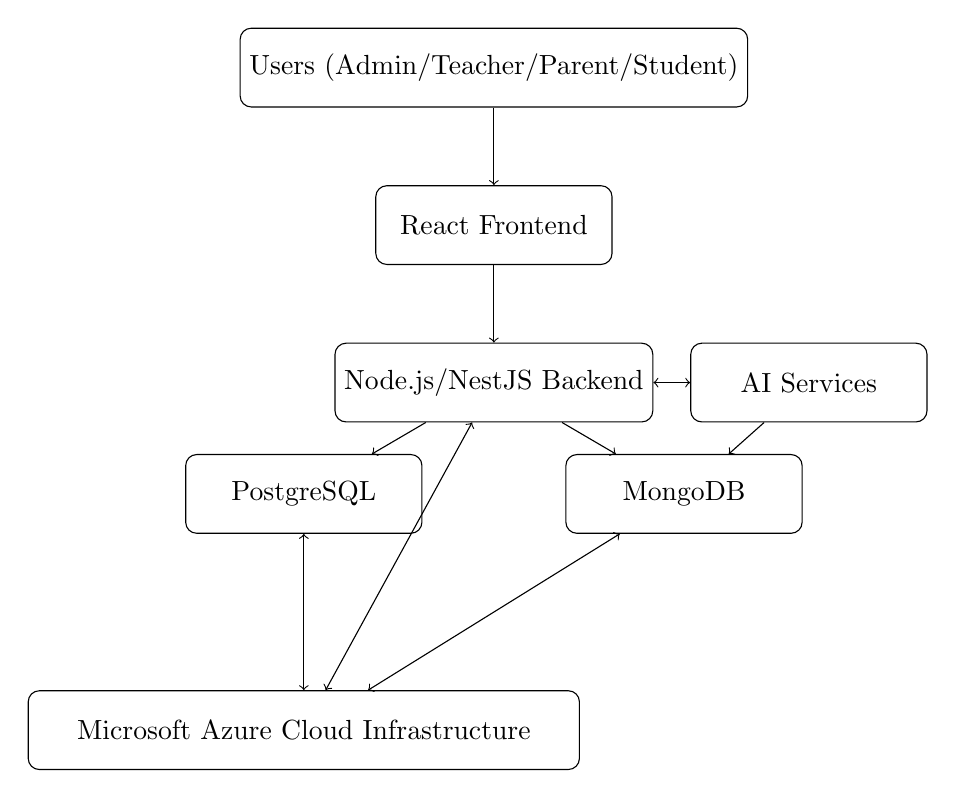
\begin{tikzpicture}[node distance=2cm]
\node (client) [rectangle, rounded corners, minimum width=3cm, minimum height=1cm, text centered, draw=black] {Users (Admin/Teacher/Parent/Student)};
\node (frontend) [rectangle, rounded corners, minimum width=3cm, minimum height=1cm, text centered, draw=black, below of=client] {React Frontend};
\node (backend) [rectangle, rounded corners, minimum width=3cm, minimum height=1cm, text centered, draw=black, below of=frontend] {Node.js/NestJS Backend};
\node (postgres) [rectangle, rounded corners, minimum width=3cm, minimum height=1cm, text centered, draw=black, below left of=backend, xshift=-1cm] {PostgreSQL};
\node (mongodb) [rectangle, rounded corners, minimum width=3cm, minimum height=1cm, text centered, draw=black, below right of=backend, xshift=1cm] {MongoDB};
\node (ai) [rectangle, rounded corners, minimum width=3cm, minimum height=1cm, text centered, draw=black, right of=backend, xshift=2cm] {AI Services};
\node (azure) [rectangle, rounded corners, minimum width=7cm, minimum height=1cm, text centered, draw=black, below of=postgres, yshift=-1cm] {Microsoft Azure Cloud Infrastructure};

\draw[->] (client) -- (frontend);
\draw[->] (frontend) -- (backend);
\draw[->] (backend) -- (postgres);
\draw[->] (backend) -- (mongodb);
\draw[<->] (backend) -- (ai);
\draw[->] (ai) -- (mongodb);
\draw[<->] (postgres) -- (azure);
\draw[<->] (mongodb) -- (azure);
\draw[<->] (backend) -- (azure);
\end{tikzpicture}
\caption{High-level system architecture integrating React frontend, Node.js/NestJS backend, databases, and Azure cloud services}
\end{figure}

\section{Complete Module Structure}

The system is organized into a comprehensive set of functional modules, each responsible for specific aspects of school management:

\begin{figure}[H]
\centering
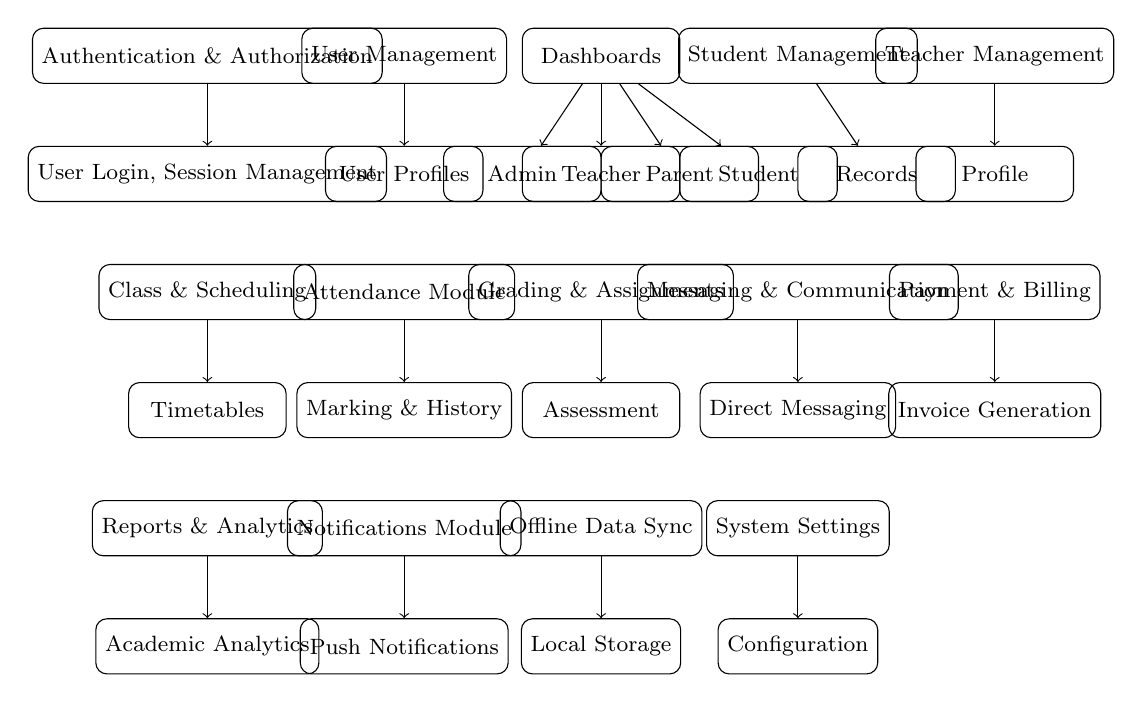
\begin{tikzpicture}[
  level 1/.style={sibling distance=20mm},
  level 2/.style={sibling distance=15mm},
  edge from parent/.style={draw,->},
  module/.style={rectangle, rounded corners, draw, align=center, minimum height=7mm, minimum width=20mm, font=\footnotesize}
]

% Top level modules
\node[module] (auth) at (0,0) {Authentication \& Authorization};
\node[module] (user) at (2.5,0) {User Management};
\node[module] (dash) at (5,0) {Dashboards};
\node[module] (student) at (7.5,0) {Student Management};
\node[module] (teacher) at (10,0) {Teacher Management};

% Second level modules
\node[module] (login) at (0,-1.5) {User Login, Session Management};
\node[module] (profiles) at (2.5,-1.5) {User Profiles};
\node[module] (admin) at (4,-1.5) {Admin};
\node[module] (teacherdash) at (5,-1.5) {Teacher};
\node[module] (parent) at (6,-1.5) {Parent};
\node[module] (studentdash) at (7,-1.5) {Student};
\node[module] (records) at (8.5,-1.5) {Records};
\node[module] (profile) at (10,-1.5) {Profile};

% Connect modules
\draw[->] (auth) -- (login);
\draw[->] (user) -- (profiles);
\draw[->] (dash) -- (admin);
\draw[->] (dash) -- (teacherdash);
\draw[->] (dash) -- (parent);
\draw[->] (dash) -- (studentdash);
\draw[->] (student) -- (records);
\draw[->] (teacher) -- (profile);

% Additional modules in next row
\node[module] (class) at (0,-3) {Class \& Scheduling};
\node[module] (attend) at (2.5,-3) {Attendance Module};
\node[module] (grade) at (5,-3) {Grading \& Assignments};
\node[module] (msg) at (7.5,-3) {Messaging \& Communication};
\node[module] (pay) at (10,-3) {Payment \& Billing};

% Connect additional modules
\node[module] (timetable) at (0,-4.5) {Timetables};
\node[module] (marking) at (2.5,-4.5) {Marking \& History};
\node[module] (assess) at (5,-4.5) {Assessment};
\node[module] (direct) at (7.5,-4.5) {Direct Messaging};
\node[module] (invoice) at (10,-4.5) {Invoice Generation};

\draw[->] (class) -- (timetable);
\draw[->] (attend) -- (marking);
\draw[->] (grade) -- (assess);
\draw[->] (msg) -- (direct);
\draw[->] (pay) -- (invoice);

% Final row of modules
\node[module] (report) at (0,-6) {Reports \& Analytics};
\node[module] (notif) at (2.5,-6) {Notifications Module};
\node[module] (offline) at (5,-6) {Offline Data Sync};
\node[module] (system) at (7.5,-6) {System Settings};

% Connect final row
\node[module] (analytics) at (0,-7.5) {Academic Analytics};
\node[module] (push) at (2.5,-7.5) {Push Notifications};
\node[module] (storage) at (5,-7.5) {Local Storage};
\node[module] (config) at (7.5,-7.5) {Configuration};

\draw[->] (report) -- (analytics);
\draw[->] (notif) -- (push);
\draw[->] (offline) -- (storage);
\draw[->] (system) -- (config);

\end{tikzpicture}
\caption{Comprehensive module structure of the school management system}
\label{fig:module_structure}
\end{figure}

\section{System Interaction Flow}

The following diagram illustrates how users interact with the system and how data flows between the various modules:

\begin{figure}[H]
\centering
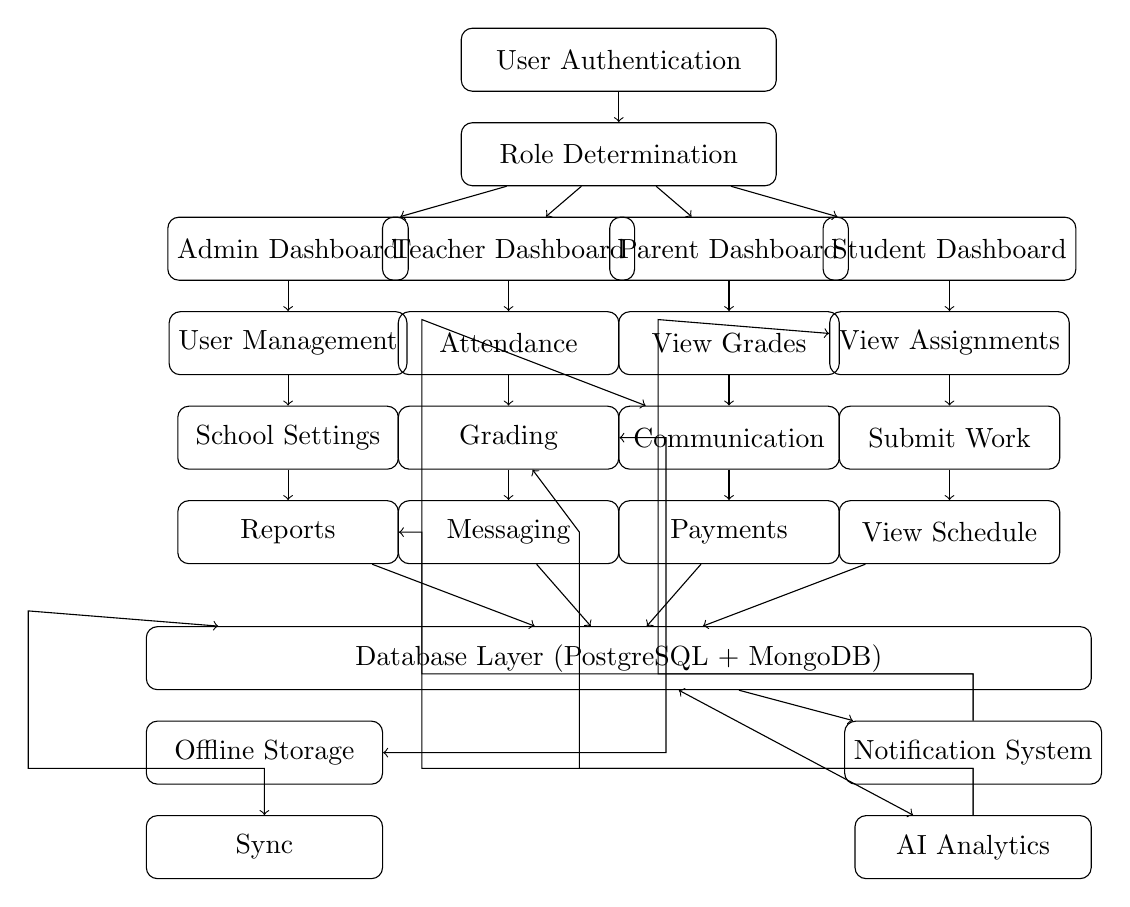
\begin{tikzpicture}[node distance=1.2cm, 
                    every node/.style={rectangle, rounded corners, draw, align=center, 
                                      minimum height=0.8cm}]

% Top row
\node[text centered, minimum width=4cm] (auth) {User Authentication};
\node[text centered, minimum width=4cm, below of=auth] (role) {Role Determination};

% Role-specific dashboards
\node[text centered, minimum width=2.8cm, below of=role, xshift=-4.2cm] (admin) {Admin Dashboard};
\node[text centered, minimum width=2.8cm, below of=role, xshift=-1.4cm] (teacher) {Teacher Dashboard};
\node[text centered, minimum width=2.8cm, below of=role, xshift=1.4cm] (parent) {Parent Dashboard};
\node[text centered, minimum width=2.8cm, below of=role, xshift=4.2cm] (student) {Student Dashboard};

% Action rows for each dashboard
\node[text centered, minimum width=2.8cm, below of=admin] (admin1) {User Management};
\node[text centered, minimum width=2.8cm, below of=admin1] (admin2) {School Settings};
\node[text centered, minimum width=2.8cm, below of=admin2] (admin3) {Reports};

\node[text centered, minimum width=2.8cm, below of=teacher] (teacher1) {Attendance};
\node[text centered, minimum width=2.8cm, below of=teacher1] (teacher2) {Grading};
\node[text centered, minimum width=2.8cm, below of=teacher2] (teacher3) {Messaging};

\node[text centered, minimum width=2.8cm, below of=parent] (parent1) {View Grades};
\node[text centered, minimum width=2.8cm, below of=parent1] (parent2) {Communication};
\node[text centered, minimum width=2.8cm, below of=parent2] (parent3) {Payments};

\node[text centered, minimum width=2.8cm, below of=student] (student1) {View Assignments};
\node[text centered, minimum width=2.8cm, below of=student1] (student2) {Submit Work};
\node[text centered, minimum width=2.8cm, below of=student2] (student3) {View Schedule};

% Database and supporting systems
\node[text centered, minimum width=12cm, below of=admin3, xshift=4.2cm, yshift=-0.4cm] (db) {Database Layer (PostgreSQL + MongoDB)};

\node[text centered, minimum width=3cm, below of=db, xshift=-4.5cm] (offline) {Offline Storage};
\node[text centered, minimum width=3cm, below of=offline] (sync) {Sync};

\node[text centered, minimum width=3cm, below of=db, xshift=4.5cm] (notif) {Notification System};
\node[text centered, minimum width=3cm, below of=notif] (ai) {AI Analytics};

% Connections
\draw[->] (auth) -- (role);
\draw[->] (role) -- (admin);
\draw[->] (role) -- (teacher);
\draw[->] (role) -- (parent);
\draw[->] (role) -- (student);

\draw[->] (admin) -- (admin1);
\draw[->] (admin1) -- (admin2);
\draw[->] (admin2) -- (admin3);

\draw[->] (teacher) -- (teacher1);
\draw[->] (teacher1) -- (teacher2);
\draw[->] (teacher2) -- (teacher3);

\draw[->] (parent) -- (parent1);
\draw[->] (parent1) -- (parent2);
\draw[->] (parent2) -- (parent3);

\draw[->] (student) -- (student1);
\draw[->] (student1) -- (student2);
\draw[->] (student2) -- (student3);

\draw[->] (admin3) -- (db);
\draw[->] (teacher3) -- (db);
\draw[->] (parent3) -- (db);
\draw[->] (student3) -- (db);

\draw[<->] (teacher2) -- ++(2,0) -- ++(0,-4) -- (offline);
\draw[->] (offline) -- (sync);
\draw[->] (sync) -- ++(0,1) -- ++(-3,0) -- ++(0,2) -- (db);

\draw[->] (db) -- (notif);
\draw[->] (notif) -- ++(0,1) -- ++(-7,0) -- ++(0,4.5) -- (parent2);
\draw[->] (notif) -- ++(0,1) -- ++(-4,0) -- ++(0,4.5) -- (student1);

\draw[<->] (db) -- (ai);
\draw[->] (ai) -- ++(0,1) -- ++(-7,0) -- ++(0,3) -- (admin3);
\draw[->] (ai) -- ++(0,1) -- ++(-5,0) -- ++(0,3) -- (teacher2);

\end{tikzpicture}
\caption{System interaction flow showing user roles, actions, and data processing}
\label{fig:system_interaction}
\end{figure}

\chapter{Implementation Roadmap}

\section{Phased Implementation Strategy}

To ensure rapid adoption and early value delivery, we recommend a phased implementation approach. This strategy allows for quick deployment of core functionality while gradually introducing more advanced features.

\begin{figure}[H]
\centering
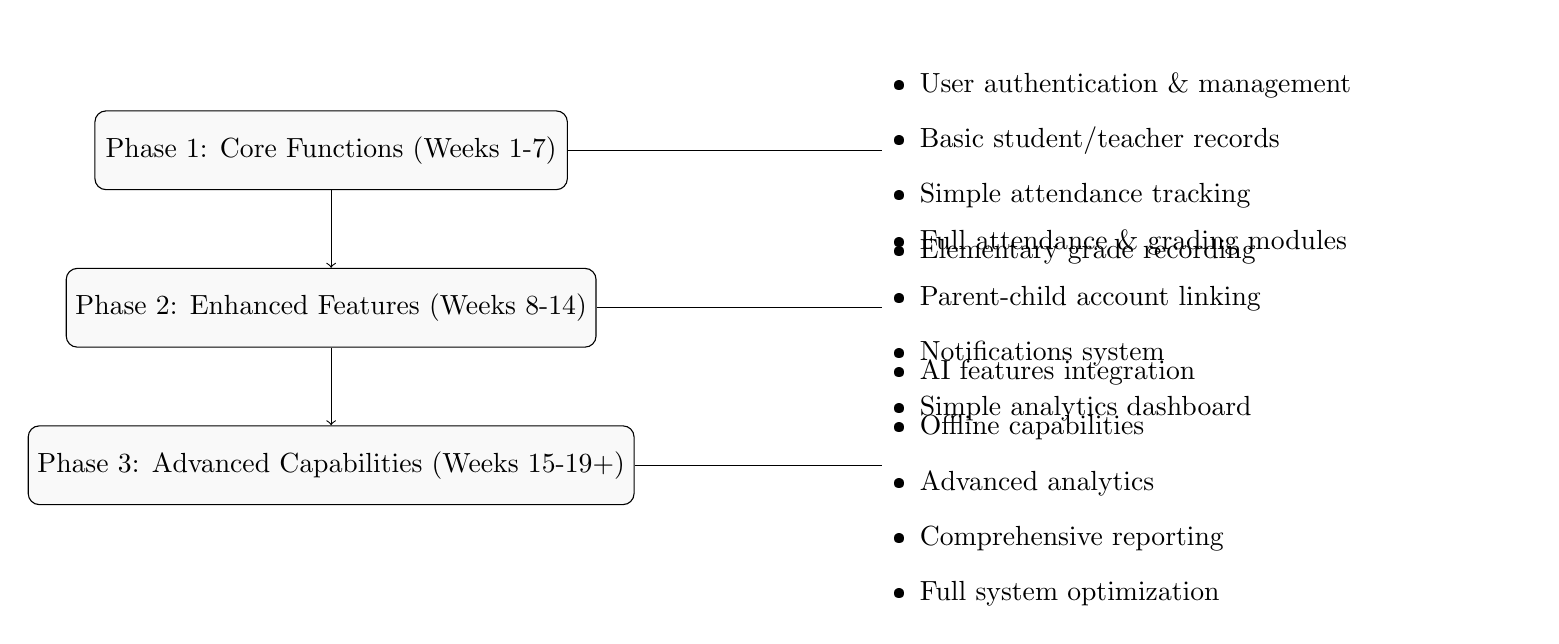
\begin{tikzpicture}[node distance=0.5cm, box/.style={rectangle, draw, rounded corners, minimum width=6cm, minimum height=1cm, text centered, fill=gray!5}]

\node[box] (phase1) at (0,0) {Phase 1: Core Functions (Weeks 1-7)};
\node[box] (phase2) at (0,-2) {Phase 2: Enhanced Features (Weeks 8-14)};
\node[box] (phase3) at (0,-4) {Phase 3: Advanced Capabilities (Weeks 15-19+)};

\node[text width=8cm, anchor=west] (phase1_details) at (7,0) {
\begin{itemize}[leftmargin=*]
\item User authentication \& management
\item Basic student/teacher records
\item Simple attendance tracking
\item Elementary grade recording
\end{itemize}
};

\node[text width=8cm, anchor=west] (phase2_details) at (7,-2) {
\begin{itemize}[leftmargin=*]
\item Full attendance \& grading modules
\item Parent-child account linking
\item Notifications system
\item Simple analytics dashboard
\end{itemize}
};

\node[text width=8cm, anchor=west] (phase3_details) at (7,-4) {
\begin{itemize}[leftmargin=*]
\item AI features integration
\item Offline capabilities
\item Advanced analytics
\item Comprehensive reporting
\item Full system optimization
\end{itemize}
};

\draw[->] (phase1) -- (phase2);
\draw[->] (phase2) -- (phase3);

\draw[-] (phase1.east) -- ++(1,0) -- (phase1_details.west);
\draw[-] (phase2.east) -- ++(1,0) -- (phase2_details.west);
\draw[-] (phase3.east) -- ++(1,0) -- (phase3_details.west);

\end{tikzpicture}
\caption{Phased implementation approach for the school management system}
\label{fig:phased_implementation}
\end{figure}

\section{Initial MVP Implementation}

The initial Minimum Viable Product (MVP) focuses on quickly delivering core functionality that provides immediate value to schools:

\begin{table}[H]
\centering
\begin{tabular}{|p{3.5cm}|p{9cm}|}
\hline
\textbf{Component} & \textbf{MVP Scope} \\
\hline
Authentication & Basic login/logout with role-based access for admins and teachers only \\
\hline
User Management & Manual creation of admin and teacher accounts; bulk upload of student records \\
\hline
Dashboards & Simple dashboards for admin and teacher access \\
\hline
Student Records & Basic student information management; class assignments \\
\hline
Attendance & Simple attendance marking interface with online-only functionality \\
\hline
Grading & Basic grade entry and simple report cards \\
\hline
Database & PostgreSQL implementation only (MongoDB integration deferred) \\
\hline
Deployment & Single-environment Azure deployment with manual scaling \\
\hline
\end{tabular}
\caption{Initial MVP scope for rapid implementation}
\end{table}

\section{Detailed Phase Roadmap}

\subsection{Phase 1: Requirements \& Design (Weeks 1-2)}
\begin{itemize}
    \item Gather detailed requirements from stakeholders
    \item Finalize feature set and refine architecture
    \item Choose specific technology components
    \item Set up project repository and structure
    \item Create detailed mockups for MVP user interfaces
\end{itemize}

\subsection{Phase 2: Initial Setup and CI/CD (Week 3)}
\begin{itemize}
    \item Initialize codebases for frontend and backend
    \item Set up development tools and code quality standards
    \item Establish CI/CD pipeline with GitHub Actions
    \item Create basic Azure development environment
    \item Set up basic project structure with module separation
\end{itemize}

\subsection{Phase 3: Core Backend Development (Weeks 4-6)}
\begin{itemize}
    \item Implement user management and authentication
    \item Set up database schemas and relationships
    \item Develop core API endpoints for basic functionality
    \item Configure role-based access control
    \item Implement bulk student upload functionality
\end{itemize}

\subsection{Phase 4: Core Frontend Development (Weeks 5-7)}
\begin{itemize}
    \item Build authentication UI and login flows
    \item Develop role-based dashboards
    \item Implement navigation and basic page structure
    \item Integrate with backend APIs
    \item Create MVP attendance and grading interfaces
\end{itemize}

\subsection{Phase 5: Feature Development (Weeks 8-11)}
\begin{itemize}
    \item Complete attendance management features with history and reporting
    \item Develop comprehensive grading and assessment modules
    \item Create notification system for important events
    \item Build basic reporting tools for administrators
    \item Implement parent-student account linking functionality
    \item Develop parent and student dashboards
\end{itemize}

\subsection{Phase 6: AI Features Integration (Weeks 12-14)}
\begin{itemize}
    \item Integrate Azure Cognitive Services for facial recognition attendance
    \item Develop analytics module for student performance insights
    \item Implement predictive modeling for identifying at-risk students
    \item Create AI-enhanced dashboards and visualizations
    \item Build intelligent reporting with trend analysis
\end{itemize}

\subsection{Phase 7: Offline Mode and PWA (Weeks 15-16)}
\begin{itemize}
    \item Implement service worker for asset caching
    \item Develop IndexedDB storage for offline data capture
    \item Create background sync mechanisms for attendance and grades
    \item Test and optimize offline workflows
    \item Implement PWA installation capabilities
\end{itemize}

\subsection{Phase 8: Testing \& Quality Assurance (Week 17)}
\begin{itemize}
    \item Conduct comprehensive testing (unit, integration, end-to-end)
    \item Perform security audits and vulnerability assessments
    \item Test performance under various conditions including poor connectivity
    \item Collect and incorporate user feedback
    \item Verify accessibility compliance
\end{itemize}

\subsection{Phase 9: Deployment \& Launch (Week 18)}
\begin{itemize}
    \item Finalize production environment on Azure
    \item Deploy application through CI/CD pipeline
    \item Conduct final validation testing
    \item Plan and execute phased rollout strategy
    \item Provide user training and documentation
\end{itemize}

\subsection{Phase 10: Post-Launch Support (Week 19+)}
\begin{itemize}
    \item Monitor system performance and user adoption
    \item Address any issues or bugs discovered
    \item Gather feedback for future improvements
    \item Plan next iteration of features
    \item Develop roadmap for additional modules (e.g., Payment & Billing)
\end{itemize}

\chapter{Technical Implementation Details}

\section{Initial MVP Implementation Details}

For the initial MVP launch (Phase 1), we will focus on implementing the following core components in a streamlined manner to ensure quick delivery of value:

\subsection{Core MVP Modules}
\begin{itemize}
    \item \textbf{Authentication:} Basic login/logout with JWT and role-based access
    \item \textbf{User Management:} Admin creation of users and bulk upload of students
    \item \textbf{Student Records:} Basic information management and class assignments
    \item \textbf{Attendance:} Simple online attendance tracking interface
    \item \textbf{Grading:} Basic grade entry and simple report cards
\end{itemize}

\begin{figure}[H]
\centering
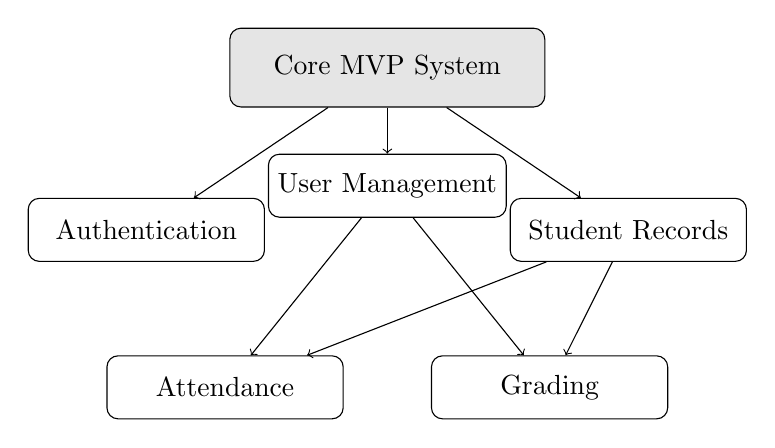
\begin{tikzpicture}[node distance=1.5cm]
\node (core) [rectangle, rounded corners, minimum width=4cm, minimum height=1cm, text centered, draw=black, fill=gray!20] {Core MVP System};

\node (auth) [rectangle, rounded corners, minimum width=3cm, minimum height=0.8cm, text centered, draw=black, below left of=core, xshift=-2cm, yshift=-1cm] {Authentication};
\node (users) [rectangle, rounded corners, minimum width=3cm, minimum height=0.8cm, text centered, draw=black, below of=core] {User Management};
\node (records) [rectangle, rounded corners, minimum width=3cm, minimum height=0.8cm, text centered, draw=black, below right of=core, xshift=2cm, yshift=-1cm] {Student Records};
\node (attend) [rectangle, rounded corners, minimum width=3cm, minimum height=0.8cm, text centered, draw=black, below left of=users, xshift=-1cm, yshift=-1.5cm] {Attendance};
\node (grade) [rectangle, rounded corners, minimum width=3cm, minimum height=0.8cm, text centered, draw=black, below right of=users, xshift=1cm, yshift=-1.5cm] {Grading};

\draw[->] (core) -- (auth);
\draw[->] (core) -- (users);
\draw[->] (core) -- (records);
\draw[->] (users) -- (attend);
\draw[->] (users) -- (grade);
\draw[->] (records) -- (attend);
\draw[->] (records) -- (grade);

\end{tikzpicture}
\caption{Initial MVP module relationships}
\end{figure}

\subsection{MVP Database Schema}
For the MVP, we will implement a simplified database schema focusing on essential tables:

\begin{figure}[H]
\centering
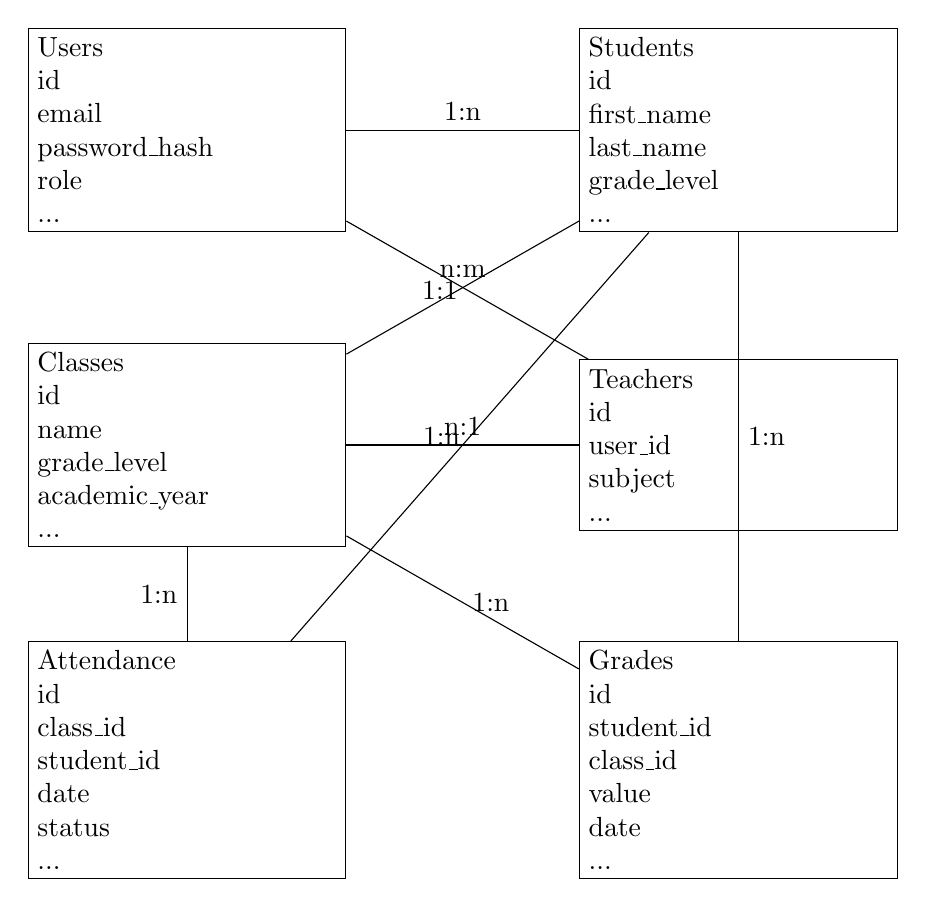
\begin{tikzpicture}[
  entity/.style={rectangle,draw,minimum width=4cm,minimum height=1.5cm,text width=3.8cm},
  relationship/.style={diamond,draw,minimum width=2.5cm,minimum height=1.5cm,text width=2.3cm,align=center},
  line/.style={-}
]

\node[entity] (users) at (0,0) {Users\\id\\email\\password\_hash\\role\\...};
\node[entity] (students) at (7,0) {Students\\id\\first\_name\\last\_name\\grade\_level\\...};
\node[entity] (classes) at (0,-4) {Classes\\id\\name\\grade\_level\\academic\_year\\...};
\node[entity] (teachers) at (7,-4) {Teachers\\id\\user\_id\\subject\\...};
\node[entity] (attendance) at (0,-8) {Attendance\\id\\class\_id\\student\_id\\date\\status\\...};
\node[entity] (grades) at (7,-8) {Grades\\id\\student\_id\\class\_id\\value\\date\\...};

\draw[line] (users) -- (students) node[midway,above] {1:n};
\draw[line] (users) -- (teachers) node[midway,left] {1:1};
\draw[line] (classes) -- (teachers) node[midway,above] {n:1};
\draw[line] (classes) -- (students) node[midway,above] {n:m};
\draw[line] (students) -- (attendance) node[midway,left] {1:n};
\draw[line] (classes) -- (attendance) node[midway,left] {1:n};
\draw[line] (students) -- (grades) node[midway,right] {1:n};
\draw[line] (classes) -- (grades) node[midway,right] {1:n};

\end{tikzpicture}
\caption{MVP database entity relationship diagram}
\end{figure}

\section{Frontend Technical Stack}

\subsection{Core Technologies}
\begin{itemize}
    \item \textbf{React:} Main library for UI development
    \item \textbf{Next.js:} Framework for server-side rendering and routing
    \item \textbf{TypeScript:} For type safety and improved developer experience
    \item \textbf{Material-UI:} Component library for consistent design
    \item \textbf{React Query:} For efficient data fetching and caching
    \item \textbf{React Context API:} For state management
    \item \textbf{Workbox:} For service worker implementation
\end{itemize}

\subsection{Frontend Organization}
The React application will follow this structure:
\begin{verbatim}
/src
  /components           # Reusable UI components
    /common             # Shared components (buttons, inputs, etc.)
    /layout             # Layout components (header, sidebar, etc.)
    /forms              # Form components
    /dashboards         # Dashboard components per role
  /hooks                # Custom React hooks
  /context              # Context providers
  /services             # API service calls
  /utils                # Utility functions
  /pages                # Next.js pages/routes
  /styles               # Global styles and themes
  /public               # Static assets
    /manifest.json      # PWA manifest
    /service-worker.js  # Service worker for offline capabilities
\end{verbatim}

\section{Backend Technical Stack}

\subsection{Core Technologies}
\begin{itemize}
    \item \textbf{Node.js:} Runtime environment
    \item \textbf{NestJS:} Backend framework
    \item \textbf{TypeScript:} For type safety
    \item \textbf{TypeORM/Prisma:} ORM for database interactions
    \item \textbf{Passport:} Authentication middleware
    \item \textbf{JWT:} For secure token-based authentication
    \item \textbf{Class-validator:} For input validation
\end{itemize}

\subsection{Backend Organization}
The NestJS application will follow this modular structure:
\begin{verbatim}
/src
  /main.ts              # Application entry point
  /app.module.ts        # Root module
  /auth                 # Authentication module
    /controllers        # Auth endpoints
    /services           # Auth business logic
    /\section{Parent Communication Workflow}

\begin{figure}[H]
\centering
\resizebox{\textwidth}{!}{
\begin{tikzpicture}[node distance=2.5cm]
\node (login) [rectangle, rounded corners, minimum width=4cm, minimum height=0.8cm, text centered, draw=black] {Parent logs into system};

\node (dashboard) [rectangle, rounded corners, minimum width=4cm, minimum height=0.8cm, text centered, draw=black, below of=login] {Parent views dashboard};

\node (child) [rectangle, rounded corners, minimum width=4cm, minimum height=0.8cm, text centered, draw=black, below of=dashboard] {Parent selects child (if multiple)};

\node (decision) [diamond, minimum width=3.5cm, minimum height=1.8cm, text centered, draw=black, below of=child, yshift=-1.2cm] {Communication\\ Type?};

\node (teacher) [rectangle, rounded corners, minimum width=4cm, minimum height=0.8cm, text centered, draw=black, below of=decision, xshift=-5cm, yshift=-1.2cm] {Message Teacher};

\node (admin) [rectangle, rounded corners, minimum width=4cm, minimum height=0.8cm, text centered, draw=black, below of=decision, xshift=5cm, yshift=-1.2cm] {Contact Administration};

\node (compose) [rectangle, rounded corners, minimum width=4cm, minimum height=0.8cm, text centered, draw=black, below of=teacher, yshift=-0.8cm] {Compose message};

\node (admin_form) [rectangle, rounded corners, minimum width=4cm, minimum height=0.8cm, text centered, draw=black, below of=admin, yshift=-0.8cm] {Fill contact form};

\node (topics) [rectangle, rounded corners, minimum width=5cm, minimum height=1.5cm, text centered, draw=black, below of=compose, yshift=-0.8cm] {- Attendance issues\\ - Academic performance\\ - Assignment clarifications};

\node (admin_topics) [rectangle, rounded corners, minimum width=5cm, minimum height=1.5cm, text centered, draw=black, below of=admin_form, yshift=-0.8cm] {- Administrative requests\\ - Account issues\\ - General feedback};

\node (follow_up) [rectangle, rounded corners, minimum width=6cm, minimum height=0.8cm, text centered, draw=black, below of=topics, xshift=2.5cm, yshift=-2cm] {Parent receives notification when response arrives};

\node (history) [rectangle, rounded corners, minimum width=6cm, minimum height=0.8cm, text centered, draw=black, below of=follow_up, yshift=-0.8cm] {Communication history available for reference};

\draw[->] (login) -- (dashboard);
\draw[->] (dashboard) -- (child);
\draw[->] (child) -- (decision);
\draw[->] (decision) -- (teacher) node[midway, above, sloped] {Teacher};
\draw[->] (decision) -- (admin) node[midway, above, sloped] {Administration};
\draw[->] (teacher) -- (compose);
\draw[->] (admin) -- (admin_form);
\draw[->] (compose) -- (topics);
\draw[->] (admin_form) -- (admin_topics);
\draw[->] (topics) |- (follow_up);
\draw[->] (admin_topics) |- (follow_up);
\draw[->] (follow_up) -- (history);
\end{tikzpicture}
}
\caption{Parent communication workflow}
\end{figure}

\section{Student Workflows}

\subsection{Student Assignment Submission Workflow}

\begin{figure}[H]
\centering
\resizebox{\textwidth}{!}{
\begin{tikzpicture}[node distance=2.5cm]
\node (login) [rectangle, rounded corners, minimum width=4cm, minimum height=0.8cm, text centered, draw=black] {Student logs into system};

\node (dashboard) [rectangle, rounded corners, minimum width=4cm, minimum height=0.8cm, text centered, draw=black, below of=login] {Student views dashboard};

\node (assignments) [rectangle, rounded corners, minimum width=4cm, minimum height=0.8cm, text centered, draw=black, below of=dashboard] {Student opens Assignments section};

\node (view) [rectangle, rounded corners, minimum width=4.5cm, minimum height=0.8cm, text centered, draw=black, below of=assignments] {Student views assignment details};

\node (work) [rectangle, rounded corners, minimum width=4.5cm, minimum height=0.8cm, text centered, draw=black, below of=view] {Student completes assignment offline};

\node (upload) [rectangle, rounded corners, minimum width=4cm, minimum height=0.8cm, text centered, draw=black, below of=work] {Student uploads work to system};

\node (decision) [diamond, minimum width=2.5cm, minimum height=1.5cm, text centered, draw=black, below of=upload, yshift=-1.2cm] {Online?};

\node (submit_online) [rectangle, rounded corners, minimum width=4cm, minimum height=0.8cm, text centered, draw=black, below of=decision, xshift=-4.5cm, yshift=-1.2cm] {Work submitted directly};

\node (store_offline) [rectangle, rounded corners, minimum width=4cm, minimum height=0.8cm, text centered, draw=black, below of=decision, xshift=4.5cm, yshift=-1.2cm] {Work stored locally in browser};

\node (confirm_online) [rectangle, rounded corners, minimum width=4cm, minimum height=0.8cm, text centered, draw=black, below of=submit_online, yshift=-0.8cm] {System confirms submission};

\node (sync) [rectangle, rounded corners, minimum width=4cm, minimum height=0.8cm, text centered, draw=black, below of=store_offline, yshift=-0.8cm] {Auto-sync when online again};

\node (teacher) [rectangle, rounded corners, minimum width=5cm, minimum height=0.8cm, text centered, draw=black, below of=confirm_online, yshift=-1.8cm] {Assignment available for teacher review};

\node (feedback) [rectangle, rounded corners, minimum width=5cm, minimum height=0.8cm, text centered, draw=black, below of=teacher, yshift=-0.8cm] {Student later receives grade and feedback};

\draw[->] (login) -- (dashboard);
\draw[->] (dashboard) -- (assignments);
\draw[->] (assignments) -- (view);
\draw[->] (view) -- (work);
\draw[->] (work) -- (upload);
\draw[->] (upload) -- (decision);
\draw[->] (decision) -- (submit_online) node[midway, above, sloped] {Yes};
\draw[->] (decision) -- (store_offline) node[midway, above, sloped] {No};
\draw[->] (submit_online) -- (confirm_online);
\draw[->] (store_offline) -- (sync);
\draw[->] (confirm_online) -- (teacher);
\draw[->] (sync) |- (teacher);
\draw[->] (teacher) -- (feedback);
\end{tikzpicture}
}
\caption{Student workflow for assignment submission}
\end{figure}

\subsection{Student Schedule and Grades Review Workflow}

\begin{figure}[H]
\centering
\resizebox{\textwidth}{!}{
\begin{tikzpicture}[node distance=2.5cm]
\node (login) [rectangle, rounded corners, minimum width=4cm, minimum height=0.8cm, text centered, draw=black] {Student logs into system};

\node (dashboard) [rectangle, rounded corners, minimum width=4cm, minimum height=0.8cm, text centered, draw=black, below of=login] {Student views dashboard};

\node (decision) [diamond, minimum width=3.2cm, minimum height=1.8cm, text centered, draw=black, below of=dashboard, yshift=-1.2cm] {Information\\ to View?};

\node (schedule) [rectangle, rounded corners, minimum width=3.5cm, minimum height=0.8cm, text centered, draw=black, below of=decision, xshift=-5.5cm, yshift=-1.2cm] {Class Schedule};

\node (grades) [rectangle, rounded corners, minimum width=3.5cm, minimum height=0.8cm, text centered, draw=black, below of=decision, yshift=-1.2cm] {Academic Grades};

\node (tasks) [rectangle, rounded corners, minimum width=3.5cm, minimum height=0.8cm, text centered, draw=black, below of=decision, xshift=5.5cm, yshift=-1.2cm] {Upcoming Tasks};

\node (view_schedule) [rectangle, rounded corners, minimum width=3.5cm, minimum height=0.8cm, text centered, draw=black, below of=schedule, yshift=-0.8cm] {Daily/weekly timetable};

\node (view_grades) [rectangle, rounded corners, minimum width=3.5cm, minimum height=0.8cm, text centered, draw=black, below of=grades, yshift=-0.8cm] {Subject-wise performance};

\node (view_tasks) [rectangle, rounded corners, minimum width=3.5cm, minimum height=0.8cm, text centered, draw=black, below of=tasks, yshift=-0.8cm] {Assignments/test dates};

\node (detail) [rectangle, rounded corners, minimum width=5cm, minimum height=0.8cm, text centered, draw=black, below of=view_grades, yshift=-1.8cm] {Student can drill down for details};

\node (action) [rectangle, rounded corners, minimum width=5.5cm, minimum height=0.8cm, text centered, draw=black, below of=detail, yshift=-0.8cm] {Student can take appropriate actions based on data};

\node (offline) [rectangle, rounded corners, minimum width=5cm, minimum height=0.8cm, text centered, draw=black, below of=action, yshift=-0.8cm] {Information available offline if previously loaded};

\draw[->] (login) -- (dashboard);
\draw[->] (dashboard) -- (decision);
\draw[->] (decision) -- (schedule) node[midway, above, sloped] {Schedule};
\draw[->] (decision) -- (grades) node[midway, above] {Grades};
\draw[->] (decision) -- (tasks) node[midway, above, sloped] {Tasks};
\draw[->] (schedule) -- (view_schedule);
\draw[->] (grades) -- (view_grades);
\draw[->] (tasks) -- (view_tasks);
\draw[->] (view_schedule) |- (detail);
\draw[->] (view_grades) -- (detail);
\draw[->] (view_tasks) |- (detail);
\draw[->] (detail) -- (action);
\draw[->] (action) -- (offline);
\end{tikzpicture}
}
\caption{Student workflow for schedule and grades review}
\end{figure}

\chapter{Key Implementation Challenges \& Mitigation Strategies}

During the implementation of the school management system, several technical and organizational challenges are anticipated. This section outlines these challenges and provides strategies to address them effectively.

\section{Technical Challenges}

\begin{table}[H]
\centering
\begin{tabular}{|p{3.5cm}|p{5.5cm}|p{5.5cm}|}
\hline
\textbf{Challenge} & \textbf{Description} & \textbf{Mitigation Strategy} \\
\hline
Data Migration & Transferring existing student, teacher, and academic records from legacy systems & \begin{itemize}
\item Develop specialized ETL scripts
\item Implement a phased migration approach
\item Provide a transitional period with both systems
\end{itemize} \\
\hline
Offline Reliability & Ensuring data integrity during offline usage and synchronization & \begin{itemize}
\item Robust conflict resolution mechanisms
\item Clear timestamp-based precedence rules
\item Comprehensive sync status indicators
\end{itemize} \\
\hline
Performance at Scale & Maintaining responsive performance with large datasets and concurrent users & \begin{itemize}
\item Implement database indexing strategies
\item Use caching for frequently accessed data
\item Design for horizontal scalability on Azure
\end{itemize} \\
\hline
AI Model Accuracy & Building accurate prediction and facial recognition models & \begin{itemize}
\item Start with conservative, high-confidence predictions
\item Continuously improve models with new data
\item Provide manual override options
\end{itemize} \\
\hline
Security & Protecting sensitive student data and preventing unauthorized access & \begin{itemize}
\item Regular security audits and penetration testing
\item End-to-end encryption for sensitive data
\item Comprehensive role-based access controls
\end{itemize} \\
\hline
\end{tabular}
\caption{Technical implementation challenges and mitigation strategies}
\end{table}

\section{Organizational Challenges}

\begin{table}[H]
\centering
\begin{tabular}{|p{3.5cm}|p{5.5cm}|p{5.5cm}|}
\hline
\textbf{Challenge} & \textbf{Description} & \textbf{Mitigation Strategy} \\
\hline
User Adoption & Ensuring stakeholders embrace and effectively use the new system & \begin{itemize}
\item Comprehensive training program
\item Intuitive UX design for minimal learning curve
\item Designated "super users" within each user group
\end{itemize} \\
\hline
Changing Requirements & Managing evolving requirements during implementation & \begin{itemize}
\item Agile methodology for adaptability
\item Regular stakeholder feedback sessions
\item Modular design for feature flexibility
\end{itemize} \\
\hline
Training & Educating staff, parents, and students on system usage & \begin{itemize}
\item Role-specific training materials and videos
\item In-app guided tours and contextual help
\item Support desk during initial deployment
\end{itemize} \\
\hline
Workflow Integration & Adapting the system to existing school processes & \begin{itemize}
\item Process mapping workshops before implementation
\item Configurable workflows in the system
\item Phased approach to process changes
\end{itemize} \\
\hline
Stakeholder Alignment & Managing expectations across diverse stakeholder groups & \begin{itemize}
\item Regular progress updates and demos
\item Clear communication about features and limitations
\item Feedback channels for continuous improvement
\end{itemize} \\
\hline
\end{tabular}
\caption{Organizational implementation challenges and mitigation strategies}
\end{table}

\chapter{Data Security \& Compliance}

Protecting sensitive student and academic data is a critical aspect of the school management system implementation. This section outlines the comprehensive security measures and compliance considerations incorporated into the design.

\section{Security Architecture}

\begin{figure}[H]
\centering
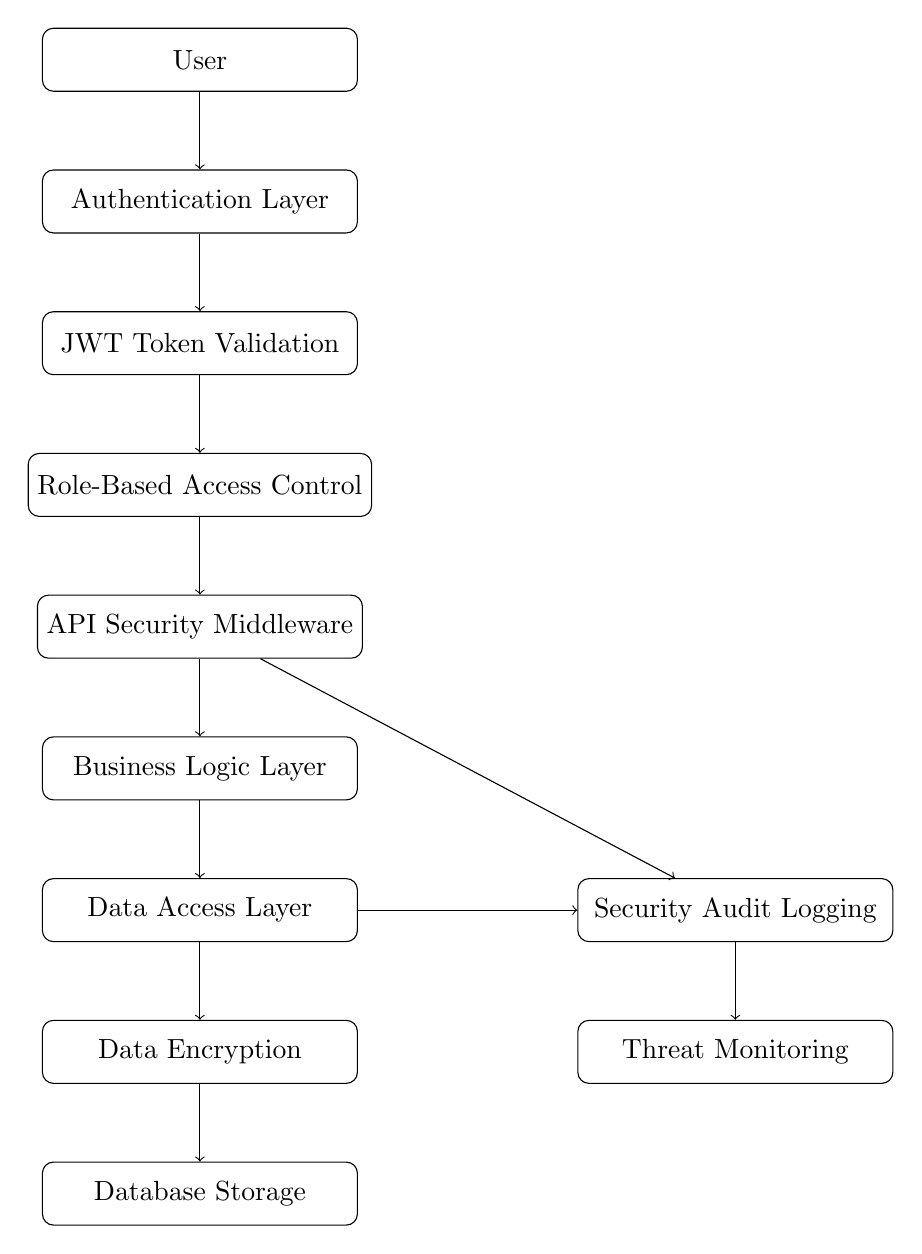
\begin{tikzpicture}[node distance=1.8cm]
\node (user) [rectangle, rounded corners, minimum width=4cm, minimum height=0.8cm, text centered, draw=black] {User};

\node (auth) [rectangle, rounded corners, minimum width=4cm, minimum height=0.8cm, text centered, draw=black, below of=user] {Authentication Layer};

\node (jwt) [rectangle, rounded corners, minimum width=4cm, minimum height=0.8cm, text centered, draw=black, below of=auth] {JWT Token Validation};

\node (rbac) [rectangle, rounded corners, minimum width=4cm, minimum height=0.8cm, text centered, draw=black, below of=jwt] {Role-Based Access Control};

\node (api) [rectangle, rounded corners, minimum width=4cm, minimum height=0.8cm, text centered, draw=black, below of=rbac] {API Security Middleware};

\node (business) [rectangle, rounded corners, minimum width=4cm, minimum height=0.8cm, text centered, draw=black, below of=api] {Business Logic Layer};

\node (data) [rectangle, rounded corners, minimum width=4cm, minimum height=0.8cm, text centered, draw=black, below of=business] {Data Access Layer};

\node (encryption) [rectangle, rounded corners, minimum width=4cm, minimum height=0.8cm, text centered, draw=black, below of=data] {Data Encryption};

\node (database) [rectangle, rounded corners, minimum width=4cm, minimum height=0.8cm, text centered, draw=black, below of=encryption] {Database Storage};

\node (logging) [rectangle, rounded corners, minimum width=4cm, minimum height=0.8cm, text centered, draw=black, right of=data, xshift=5cm] {Security Audit Logging};

\node (monitoring) [rectangle, rounded corners, minimum width=4cm, minimum height=0.8cm, text centered, draw=black, below of=logging] {Threat Monitoring};

\draw[->] (user) -- (auth);
\draw[->] (auth) -- (jwt);
\draw[->] (jwt) -- (rbac);
\draw[->] (rbac) -- (api);
\draw[->] (api) -- (business);
\draw[->] (business) -- (data);
\draw[->] (data) -- (encryption);
\draw[->] (encryption) -- (database);
\draw[->] (api) -- (logging);
\draw[->] (data) -- (logging);
\draw[->] (logging) -- (monitoring);

\end{tikzpicture}
\caption{Security architecture of the school management system}
\end{figure}

\section{Security Measures}

\begin{itemize}
    \item \textbf{Authentication:} Multi-factor authentication for administrative accounts, strong password policies, and secure password reset mechanisms.
    
    \item \textbf{Authorization:} Granular role-based access control ensuring users only access data appropriate to their role.
    
    \item \textbf{Data Encryption:} All sensitive data encrypted both in transit (HTTPS/TLS) and at rest (AES-256 encryption).
    
    \item \textbf{Secure APIs:} API endpoints protected against common vulnerabilities (injection, XSS, CSRF) with input validation and sanitization.
    
    \item \textbf{Audit Logging:} Comprehensive logging of all security-relevant events and access to sensitive data.
    
    \item \textbf{Regular Security Testing:} Scheduled penetration testing and vulnerability assessments.
    
    \item \textbf{Secure Development:} Following secure coding practices and regular dependency vulnerability scanning.
    
    \item \textbf{Data Minimization:} Collecting and storing only necessary data to reduce exposure risk.
\end{itemize}

\section{Compliance Considerations}

\begin{table}[H]
\centering
\begin{tabular}{|p{3cm}|p{11.5cm}|}
\hline
\textbf{Regulation} & \textbf{Implementation Approach} \\
\hline
FERPA (USA) & \begin{itemize}
\item Parental consent for sharing student information
\item Audit trails for all data access
\item Strict access controls limiting data visibility
\item Ability to generate compliance reports
\end{itemize} \\
\hline
GDPR (EU) & \begin{itemize}
\item Data processing consent management
\item Right to access, rectification, and erasure mechanisms
\item Data breach notification capabilities
\item Data retention policies and automated purging
\end{itemize} \\
\hline
COPPA (USA) & \begin{itemize}
\item Age verification for student accounts
\item Parental consent management
\item Limited data collection from minors
\item Simplified privacy notices
\end{itemize} \\
\hline
Local Education Laws & \begin{itemize}
\item Configurable data retention policies
\item Compliance reporting capabilities
\item Adaptable privacy controls for regional requirements
\end{itemize} \\
\hline
\end{tabular}
\caption{Compliance considerations and implementation approaches}
\end{table}    /guards             # Role-based guards
  /users                # User management module
  /classes              # Class management module
  /attendance           # Attendance module
  /grades               # Grading module
  /notifications        # Notification module
  /reports              # Reporting module
  /analytics            # Analytics and AI module
  /common               # Shared utilities and interfaces
\end{verbatim}

\section{Database Schemas}

\subsection{PostgreSQL Entity Relationships}
Key entity relationships include:
\begin{itemize}
    \item Users with role-based differentiation
    \item One-to-many relationship between Teachers and Classes
    \item Many-to-many relationship between Students and Classes (via Enrollments)
    \item One-to-many relationship between Classes and Assignments
    \item One-to-many relationship between Students and Grades
\end{itemize}

\subsection{MongoDB Collections}
\begin{itemize}
    \item \textbf{Logs:} System events, user actions, errors
    \item \textbf{Analytics:} Computed insights and aggregated data
    \item \textbf{OfflineSync:} Temporary storage for offline actions
    \item \textbf{AIInsights:} Machine learning results and predictions
\end{itemize}

\section{API Design}

\subsection{RESTful Endpoints}
The API follows RESTful principles with these key endpoints:

\begin{itemize}
    \item \textbf{Authentication:} \texttt{/api/v1/auth/login}, \texttt{/api/v1/auth/refresh}
    \item \textbf{User Management:} \texttt{/api/v1/users}, \texttt{/api/v1/users/:id}
    \item \textbf{Classes:} \texttt{/api/v1/classes}, \texttt{/api/v1/classes/:id}
    \item \textbf{Students:} \texttt{/api/v1/students}, \texttt{/api/v1/classes/:id/students}
    \item \textbf{Attendance:} \texttt{/api/v1/attendance}, \texttt{/api/v1/attendance/batch}
    \item \textbf{Grades:} \texttt{/api/v1/grades}, \texttt{/api/v1/students/:id/grades}
    \item \textbf{Notifications:} \texttt{/api/v1/notifications}, \texttt{/api/v1/users/:id/notifications}
    \item \textbf{Reports:} \texttt{/api/v1/reports/attendance}, \texttt{/api/v1/reports/performance}
    \item \textbf{AI Services:} \texttt{/api/v1/ai/face-recognition}, \texttt{/api/v1/ai/analytics}
\end{itemize}

\subsection{Authentication Flow}
\begin{enumerate}
    \item User submits credentials
    \item Server validates and issues JWT token with appropriate role claims
    \item Client stores token securely and includes in Authorization header
    \item Protected endpoints verify token and roles before processing
    \item Refresh tokens handle session extension without re-login
\end{enumerate}

\section{Azure Cloud Architecture}

\subsection{Containerization Strategy}
\begin{itemize}
    \item Application components packaged as Docker containers
    \item Container images stored in Azure Container Registry
    \item Orchestration through Azure Kubernetes Service
    \item Horizontal scaling based on demand metrics
\end{itemize}

\subsection{Azure Resources}
\begin{figure}[H]
\centering
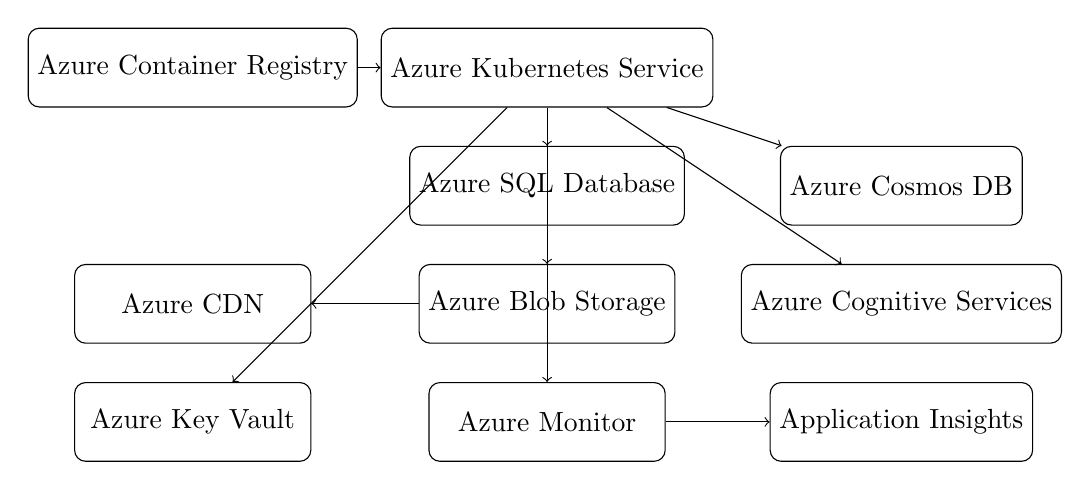
\begin{tikzpicture}[node distance=1.5cm]
\node (aks) [rectangle, rounded corners, minimum width=3cm, minimum height=1cm, text centered, draw=black] {Azure Kubernetes Service};
\node (acr) [rectangle, rounded corners, minimum width=3cm, minimum height=1cm, text centered, draw=black, left of=aks, xshift=-3cm] {Azure Container Registry};
\node (sql) [rectangle, rounded corners, minimum width=3cm, minimum height=1cm, text centered, draw=black, below of=aks] {Azure SQL Database};
\node (cosmos) [rectangle, rounded corners, minimum width=3cm, minimum height=1cm, text centered, draw=black, right of=sql, xshift=3cm] {Azure Cosmos DB};
\node (storage) [rectangle, rounded corners, minimum width=3cm, minimum height=1cm, text centered, draw=black, below of=sql] {Azure Blob Storage};
\node (cdn) [rectangle, rounded corners, minimum width=3cm, minimum height=1cm, text centered, draw=black, left of=storage, xshift=-3cm] {Azure CDN};
\node (cog) [rectangle, rounded corners, minimum width=3cm, minimum height=1cm, text centered, draw=black, right of=storage, xshift=3cm] {Azure Cognitive Services};
\node (monitor) [rectangle, rounded corners, minimum width=3cm, minimum height=1cm, text centered, draw=black, below of=storage] {Azure Monitor};
\node (keyvault) [rectangle, rounded corners, minimum width=3cm, minimum height=1cm, text centered, draw=black, left of=monitor, xshift=-3cm] {Azure Key Vault};
\node (appinsights) [rectangle, rounded corners, minimum width=3cm, minimum height=1cm, text centered, draw=black, right of=monitor, xshift=3cm] {Application Insights};

\draw[->] (acr) -- (aks);
\draw[->] (aks) -- (sql);
\draw[->] (aks) -- (cosmos);
\draw[->] (aks) -- (storage);
\draw[->] (storage) -- (cdn);
\draw[->] (aks) -- (cog);
\draw[->] (aks) -- (monitor);
\draw[->] (aks) -- (keyvault);
\draw[->] (monitor) -- (appinsights);
\end{tikzpicture}
\caption{Azure resources for school management system deployment}
\end{figure}

\subsection{Deployment Pipeline}
\begin{itemize}
    \item Source code managed in GitHub repository
    \item Automated testing with GitHub Actions
    \item Continuous integration building Docker images
    \item Continuous deployment to Azure environments
    \item Separate environments for development, staging, and production
    \item Infrastructure as Code using Azure Resource Manager templates
\end{itemize}

\chapter{User Workflows}

This chapter details the typical user interaction flows for each type of user in the system.

\section{Teacher Workflows}

\subsection{Attendance Tracking Workflow}

\begin{figure}[H]
\centering
\resizebox{\textwidth}{!}{
\begin{tikzpicture}[node distance=2.5cm]
\node (login) [rectangle, rounded corners, minimum width=4cm, minimum height=0.8cm, text centered, draw=black] {Teacher logs into the system};

\node (dashboard) [rectangle, rounded corners, minimum width=4cm, minimum height=0.8cm, text centered, draw=black, below of=login] {Teacher accesses dashboard};

\node (class) [rectangle, rounded corners, minimum width=4cm, minimum height=0.8cm, text centered, draw=black, below of=dashboard] {Teacher selects class to manage};

\node (attendance) [rectangle, rounded corners, minimum width=4cm, minimum height=0.8cm, text centered, draw=black, below of=class] {Teacher opens attendance module};

\node (decision) [diamond, minimum width=2.5cm, minimum height=1.5cm, text centered, draw=black, below of=attendance, yshift=-1.2cm] {Online?};

\node (mark_online) [rectangle, rounded corners, minimum width=4cm, minimum height=0.8cm, text centered, draw=black, below of=decision, xshift=-4.5cm, yshift=-1.2cm] {Mark attendance directly in system};

\node (mark_offline) [rectangle, rounded corners, minimum width=4cm, minimum height=0.8cm, text centered, draw=black, below of=decision, xshift=4.5cm, yshift=-1.2cm] {Mark attendance in offline mode};

\node (save_online) [rectangle, rounded corners, minimum width=4cm, minimum height=0.8cm, text centered, draw=black, below of=mark_online, yshift=-0.5cm] {Data saved to database immediately};

\node (save_offline) [rectangle, rounded corners, minimum width=4cm, minimum height=0.8cm, text centered, draw=black, below of=mark_offline, yshift=-0.5cm] {Data stored in IndexedDB};

\node (sync) [rectangle, rounded corners, minimum width=4cm, minimum height=0.8cm, text centered, draw=black, below of=save_offline, yshift=-0.5cm] {Auto-sync when back online};

\node (notify) [rectangle, rounded corners, minimum width=6cm, minimum height=0.8cm, text centered, draw=black, below of=save_online, xshift=4.5cm, yshift=-1.8cm] {System sends notifications to parents of absent students};

\node (report) [rectangle, rounded corners, minimum width=6cm, minimum height=0.8cm, text centered, draw=black, below of=notify, yshift=-0.8cm] {Attendance data available for reporting and analytics};

\draw[->] (login) -- (dashboard);
\draw[->] (dashboard) -- (class);
\draw[->] (class) -- (attendance);
\draw[->] (attendance) -- (decision);
\draw[->] (decision) -- (mark_online) node[midway, above, sloped] {Yes};
\draw[->] (decision) -- (mark_offline) node[midway, above, sloped] {No};
\draw[->] (mark_online) -- (save_online);
\draw[->] (mark_offline) -- (save_offline);
\draw[->] (save_offline) -- (sync);
\draw[->] (save_online) -- (notify);
\draw[->] (sync) -- (notify);
\draw[->] (notify) -- (report);
\end{tikzpicture}
}
\caption{Teacher workflow for attendance tracking}
\end{figure}

\subsection{Grade Entry Workflow}

\begin{figure}[H]
\centering
\resizebox{\textwidth}{!}{
\begin{tikzpicture}[node distance=2.5cm]
\node (login) [rectangle, rounded corners, minimum width=4cm, minimum height=0.8cm, text centered, draw=black] {Teacher logs into the system};

\node (dashboard) [rectangle, rounded corners, minimum width=4cm, minimum height=0.8cm, text centered, draw=black, below of=login] {Teacher accesses dashboard};

\node (class) [rectangle, rounded corners, minimum width=4cm, minimum height=0.8cm, text centered, draw=black, below of=dashboard] {Teacher selects class to manage};

\node (grades) [rectangle, rounded corners, minimum width=4cm, minimum height=0.8cm, text centered, draw=black, below of=class] {Teacher opens grading module};

\node (create) [rectangle, rounded corners, minimum width=4.5cm, minimum height=0.8cm, text centered, draw=black, below of=grades] {Teacher creates new assignment/test};

\node (enter) [rectangle, rounded corners, minimum width=4cm, minimum height=0.8cm, text centered, draw=black, below of=create] {Teacher enters grades for students};

\node (decision) [diamond, minimum width=2.5cm, minimum height=1.5cm, text centered, draw=black, below of=enter, yshift=-1.2cm] {Online?};

\node (save_online) [rectangle, rounded corners, minimum width=4cm, minimum height=0.8cm, text centered, draw=black, below of=decision, xshift=-4.5cm, yshift=-1.2cm] {Grades saved directly to database};

\node (save_offline) [rectangle, rounded corners, minimum width=4cm, minimum height=0.8cm, text centered, draw=black, below of=decision, xshift=4.5cm, yshift=-1.2cm] {Grades stored locally in IndexedDB};

\node (sync) [rectangle, rounded corners, minimum width=4cm, minimum height=0.8cm, text centered, draw=black, below of=save_offline, yshift=-0.5cm] {Auto-sync when connectivity returns};

\node (analyze) [rectangle, rounded corners, minimum width=4cm, minimum height=0.8cm, text centered, draw=black, below of=save_online, yshift=-1.8cm] {System analyzes grade patterns};

\node (notify) [rectangle, rounded corners, minimum width=4.5cm, minimum height=0.8cm, text centered, draw=black, below of=analyze, yshift=-0.8cm] {Parents/students notified of new grades};

\node (report) [rectangle, rounded corners, minimum width=4cm, minimum height=0.8cm, text centered, draw=black, below of=notify, yshift=-0.8cm] {Grades visible in performance reports};

\draw[->] (login) -- (dashboard);
\draw[->] (dashboard) -- (class);
\draw[->] (class) -- (grades);
\draw[->] (grades) -- (create);
\draw[->] (create) -- (enter);
\draw[->] (enter) -- (decision);
\draw[->] (decision) -- (save_online) node[midway, above, sloped] {Yes};
\draw[->] (decision) -- (save_offline) node[midway, above, sloped] {No};
\draw[->] (save_offline) -- (sync);
\draw[->] (sync) |- (analyze);
\draw[->] (save_online) -- (analyze);
\draw[->] (analyze) -- (notify);
\draw[->] (notify) -- (report);
\end{tikzpicture}
}
\caption{Teacher workflow for grade entry and management}
\end{figure}

\section{Administrator Workflows}

\subsection{Student Registration Workflow}

\begin{figure}[H]
\centering
\resizebox{\textwidth}{!}{
\begin{tikzpicture}[node distance=2.5cm]
\node (login) [rectangle, rounded corners, minimum width=4cm, minimum height=0.8cm, text centered, draw=black] {Admin logs into the system};

\node (dashboard) [rectangle, rounded corners, minimum width=4cm, minimum height=0.8cm, text centered, draw=black, below of=login] {Admin accesses dashboard};

\node (student) [rectangle, rounded corners, minimum width=4cm, minimum height=0.8cm, text centered, draw=black, below of=dashboard] {Admin selects Student Management};

\node (decision) [diamond, minimum width=3cm, minimum height=1.8cm, text centered, draw=black, below of=student, yshift=-1.2cm] {Single or \\ Bulk?};

\node (single) [rectangle, rounded corners, minimum width=4cm, minimum height=0.8cm, text centered, draw=black, below of=decision, xshift=-5cm, yshift=-1.2cm] {Admin fills student form manually};

\node (bulk) [rectangle, rounded corners, minimum width=4cm, minimum height=0.8cm, text centered, draw=black, below of=decision, xshift=5cm, yshift=-1.2cm] {Admin uploads CSV/Excel file};

\node (manual_save) [rectangle, rounded corners, minimum width=4cm, minimum height=0.8cm, text centered, draw=black, below of=single, yshift=-0.8cm] {System validates and saves record};

\node (process) [rectangle, rounded corners, minimum width=4cm, minimum height=0.8cm, text centered, draw=black, below of=bulk, yshift=-0.8cm] {System processes file rows};

\node (validation) [rectangle, rounded corners, minimum width=4cm, minimum height=0.8cm, text centered, draw=black, below of=process, yshift=-0.8cm] {System validates all entries};

\node (report_single) [rectangle, rounded corners, minimum width=4cm, minimum height=0.8cm, text centered, draw=black, below of=manual_save, yshift=-0.8cm] {Confirmation shown to admin};

\node (import) [rectangle, rounded corners, minimum width=4cm, minimum height=0.8cm, text centered, draw=black, below of=validation, yshift=-0.8cm] {Valid records imported to database};

\node (report_bulk) [rectangle, rounded corners, minimum width=5cm, minimum height=0.8cm, text centered, draw=black, below of=import, yshift=-0.8cm] {Import summary report displayed};

\node (account) [rectangle, rounded corners, minimum width=6cm, minimum height=0.8cm, text centered, draw=black, below of=report_single, xshift=4.5cm, yshift=-2cm] {Student accounts marked as pending activation};

\node (notify) [rectangle, rounded corners, minimum width=6cm, minimum height=0.8cm, text centered, draw=black, below of=account, yshift=-0.8cm] {Optional: Welcome emails sent to parents/students};

\draw[->] (login) -- (dashboard);
\draw[->] (dashboard) -- (student);
\draw[->] (student) -- (decision);
\draw[->] (decision) -- (single) node[midway, above, sloped] {Single};
\draw[->] (decision) -- (bulk) node[midway, above, sloped] {Bulk};
\draw[->] (single) -- (manual_save);
\draw[->] (bulk) -- (process);
\draw[->] (process) -- (validation);
\draw[->] (validation) -- (import);
\draw[->] (import) -- (report_bulk);
\draw[->] (manual_save) -- (report_single);
\draw[->] (report_single) |- (account);
\draw[->] (report_bulk) |- (account);
\draw[->] (account) -- (notify);
\end{tikzpicture}
}
\caption{Administrator workflow for student registration}
\end{figure}

\subsection{Report Generation Workflow}

\begin{figure}[H]
\centering
\resizebox{\textwidth}{!}{
\begin{tikzpicture}[node distance=2.5cm]
\node (login) [rectangle, rounded corners, minimum width=4cm, minimum height=0.8cm, text centered, draw=black] {Admin logs into the system};

\node (dashboard) [rectangle, rounded corners, minimum width=4cm, minimum height=0.8cm, text centered, draw=black, below of=login] {Admin accesses dashboard};

\node (reports) [rectangle, rounded corners, minimum width=4cm, minimum height=0.8cm, text centered, draw=black, below of=dashboard] {Admin opens Reports module};

\node (select) [rectangle, rounded corners, minimum width=4cm, minimum height=0.8cm, text centered, draw=black, below of=reports] {Admin selects report type};

\node (params) [rectangle, rounded corners, minimum width=4.5cm, minimum height=0.8cm, text centered, draw=black, below of=select] {Admin configures report parameters};

\node (generate) [rectangle, rounded corners, minimum width=4cm, minimum height=0.8cm, text centered, draw=black, below of=params] {Admin generates report};

\node (process) [rectangle, rounded corners, minimum width=4.5cm, minimum height=0.8cm, text centered, draw=black, below of=generate] {System processes data and analytics};

\node (decision) [diamond, minimum width=3.2cm, minimum height=1.8cm, text centered, draw=black, below of=process, yshift=-1.2cm] {Output Format?};

\node (view) [rectangle, rounded corners, minimum width=4cm, minimum height=0.8cm, text centered, draw=black, below of=decision, xshift=-5cm, yshift=-1.2cm] {View in browser dashboard};

\node (export) [rectangle, rounded corners, minimum width=4cm, minimum height=0.8cm, text centered, draw=black, below of=decision, xshift=5cm, yshift=-1.2cm] {Export as PDF/Excel};

\node (interact) [rectangle, rounded corners, minimum width=4cm, minimum height=0.8cm, text centered, draw=black, below of=view, yshift=-0.8cm] {Interactive visualization};

\node (download) [rectangle, rounded corners, minimum width=4cm, minimum height=0.8cm, text centered, draw=black, below of=export, yshift=-0.8cm] {File download};

\node (share) [rectangle, rounded corners, minimum width=5cm, minimum height=0.8cm, text centered, draw=black, below of=interact, xshift=2.5cm, yshift=-2cm] {Option to share with stakeholders};

\draw[->] (login) -- (dashboard);
\draw[->] (dashboard) -- (reports);
\draw[->] (reports) -- (select);
\draw[->] (select) -- (params);
\draw[->] (params) -- (generate);
\draw[->] (generate) -- (process);
\draw[->] (process) -- (decision);
\draw[->] (decision) -- (view) node[midway, above, sloped] {Browser};
\draw[->] (decision) -- (export) node[midway, above, sloped] {File};
\draw[->] (view) -- (interact);
\draw[->] (export) -- (download);
\draw[->] (interact) -- (share);
\draw[->] (download) -- (share);
\end{tikzpicture}
}
\caption{Administrator workflow for report generation}
\end{figure}

\section{Parent Workflows}

\subsection{Parent Registration and Child Linking Workflow}

\begin{landscape}
\begin{figure}
\centering
\begin{tikzpicture}[node distance=3cm]
\node (start) [rectangle, rounded corners, minimum width=4cm, minimum height=0.8cm, text centered, draw=black] {Parent visits school portal};

\node (register) [rectangle, rounded corners, minimum width=4cm, minimum height=0.8cm, text centered, draw=black, right of=start] {Parent creates new account};

\node (credentials) [rectangle, rounded corners, minimum width=4.5cm, minimum height=0.8cm, text centered, draw=black, right of=register] {Parent enters personal information};

\node (verify) [rectangle, rounded corners, minimum width=4.5cm, minimum height=0.8cm, text centered, draw=black, below of=credentials] {Email verification sent to parent};

\node (confirm) [rectangle, rounded corners, minimum width=4cm, minimum height=0.8cm, text centered, draw=black, below of=verify] {Parent confirms email};

\node (login) [rectangle, rounded corners, minimum width=4cm, minimum height=0.8cm, text centered, draw=black, below of=confirm] {Parent logs into account};

\node (link) [rectangle, rounded corners, minimum width=4.5cm, minimum height=0.8cm, text centered, draw=black, below of=login] {Parent navigates to "Link Child" page};

\node (info) [rectangle, rounded corners, minimum width=5.5cm, minimum height=0.8cm, text centered, draw=black, below of=link] {Parent enters student ID and verification info};

\node (student_check) [diamond, minimum width=2.8cm, minimum height=1.8cm, text centered, draw=black, below of=info, yshift=-1cm] {Valid Student?};

\node (error) [rectangle, rounded corners, minimum width=4cm, minimum height=0.8cm, text centered, draw=black, left of=student_check, xshift=-3cm] {Error message displayed};

\node (system_link) [rectangle, rounded corners, minimum width=4.5cm, minimum height=0.8cm, text centered, draw=black, below of=student_check, yshift=-1.2cm] {System links parent to student};

\node (approval) [diamond, minimum width=3.2cm, minimum height=2cm, text centered, draw=black, below of=system_link, yshift=-1.2cm] {Admin Approval\\ Required?};

\node (pending) [rectangle, rounded corners, minimum width=4.5cm, minimum height=0.8cm, text centered, draw=black, left of=approval, xshift=-3cm] {Link pending admin approval};

\node (admin_review) [rectangle, rounded corners, minimum width=4cm, minimum height=0.8cm, text centered, draw=black, below of=pending] {Admin reviews request};

\node (approval_decision) [diamond, minimum width=2.8cm, minimum height=1.8cm, text centered, draw=black, below of=admin_review, yshift=-1cm] {Approved?};

\node (decline) [rectangle, rounded corners, minimum width=4cm, minimum height=0.8cm, text centered, draw=black, left of=approval_decision, xshift=-3cm] {Link rejected};

\node (immediate) [rectangle, rounded corners, minimum width=4.5cm, minimum height=0.8cm, text centered, draw=black, right of=approval, xshift=3cm] {Link approved immediately};

\node (access) [rectangle, rounded corners, minimum width=5cm, minimum height=0.8cm, text centered, draw=black, below of=immediate, yshift=-3cm] {Parent granted access to child's data};

\node (dashboard) [rectangle, rounded corners, minimum width=5cm, minimum height=0.8cm, text centered, draw=black, below of=access] {Parent views child's dashboard};

\draw[->] (start) -- (register);
\draw[->] (register) -- (credentials);
\draw[->] (credentials) -- (verify);
\draw[->] (verify) -- (confirm);
\draw[->] (confirm) -- (login);
\draw[->] (login) -- (link);
\draw[->] (link) -- (info);
\draw[->] (info) -- (student_check);
\draw[->] (student_check) -- (error) node[midway, above] {No};
\draw[->] (error) |- (info);
\draw[->] (student_check) -- (system_link) node[midway, right] {Yes};
\draw[->] (system_link) -- (approval);
\draw[->] (approval) -- (immediate) node[midway, above] {No};
\draw[->] (approval) -- (pending) node[midway, above] {Yes};
\draw[->] (pending) -- (admin_review);
\draw[->] (admin_review) -- (approval_decision);
\draw[->] (approval_decision) -- (decline) node[midway, above] {No};
\draw[->] (approval_decision) |- (access) node[pos=0.25, above] {Yes};
\draw[->] (immediate) -- (access);
\draw[->] (access) -- (dashboard);

\end{tikzpicture}
\caption{Parent registration and child linking workflow}
\end{figure}
\end{landscape}

\subsection{Parent Monitoring Child's Progress Workflow}

\begin{figure}[H]
\centering
\resizebox{\textwidth}{!}{
\begin{tikzpicture}[node distance=2.5cm]
\node (login) [rectangle, rounded corners, minimum width=4cm, minimum height=0.8cm, text centered, draw=black] {Parent logs into system};

\node (dashboard) [rectangle, rounded corners, minimum width=4cm, minimum height=0.8cm, text centered, draw=black, below of=login] {Parent views dashboard};

\node (select) [rectangle, rounded corners, minimum width=4cm, minimum height=0.8cm, text centered, draw=black, below of=dashboard] {Parent selects child (if multiple)};

\node (overview) [rectangle, rounded corners, minimum width=4.5cm, minimum height=0.8cm, text centered, draw=black, below of=select] {Parent views child's overview};

\node (decision) [diamond, minimum width=3.2cm, minimum height=1.8cm, text centered, draw=black, below of=overview, yshift=-1.2cm] {Area to\\ Review?};

\node (grades) [rectangle, rounded corners, minimum width=3.5cm, minimum height=0.8cm, text centered, draw=black, below of=decision, xshift=-5.5cm, yshift=-1.2cm] {Academic Performance};

\node (attendance) [rectangle, rounded corners, minimum width=3.5cm, minimum height=0.8cm, text centered, draw=black, below of=decision, yshift=-1.2cm] {Attendance History};

\node (behavior) [rectangle, rounded corners, minimum width=3.5cm, minimum height=0.8cm, text centered, draw=black, below of=decision, xshift=5.5cm, yshift=-1.2cm] {Upcoming Tasks};

\node (grade_detail) [rectangle, rounded corners, minimum width=3.5cm, minimum height=0.8cm, text centered, draw=black, below of=grades, yshift=-0.8cm] {Review grades and feedback};

\node (attend_detail) [rectangle, rounded corners, minimum width=3.5cm, minimum height=0.8cm, text centered, draw=black, below of=attendance, yshift=-0.8cm] {View attendance patterns};

\node (task_detail) [rectangle, rounded corners, minimum width=3.5cm, minimum height=0.8cm, text centered, draw=black, below of=behavior, yshift=-0.8cm] {Check assignments/exams};

\node (contact) [rectangle, rounded corners, minimum width=5cm, minimum height=0.8cm, text centered, draw=black, below of=attend_detail, yshift=-2cm] {Option to contact teacher directly};

\node (download) [rectangle, rounded corners, minimum width=5cm, minimum height=0.8cm, text centered, draw=black, below of=contact, yshift=-0.8cm] {Download/print reports if needed};

\draw[->] (login) -- (dashboard);
\draw[->] (dashboard) -- (select);
\draw[->] (select) -- (overview);
\draw[->] (overview) -- (decision);
\draw[->] (decision) -- (grades) node[midway, above, sloped] {Grades};
\draw[->] (decision) -- (attendance) node[midway, above] {Attendance};
\draw[->] (decision) -- (behavior) node[midway, above, sloped] {Tasks};
\draw[->] (grades) -- (grade_detail);
\draw[->] (attendance) -- (attend_detail);
\draw[->] (behavior) -- (task_detail);
\draw[->] (grade_detail) |- (contact);
\draw[->] (attend_detail) -- (contact);
\draw[->] (task_detail) |- (contact);
\draw[->] (contact) -- (download);
\end{tikzpicture}
}
\caption{Parent workflow for monitoring child's progress}
\end{figure}

\subsection{Parent Communication Workflow}

\begin{figure}[H]
\centering
\resizebox{\textwidth}{!}{
\begin{tikzpicture}[node distance=2.5cm]
\node (login) [rectangle, rounded corners, minimum width=4cm, minimum height=0.8cm, text centered, draw=black] {Parent logs into system};

\node (dashboard) [rectangle, rounded corners, minimum width=4cm, minimum height=0.8cm, text centered, draw=black, below of=login] {Parent views dashboard};

\node (child) [rectangle, rounded corners, minimum width=4cm, minimum height=0.8cm, text centered, draw=black, below of=dashboard] {Parent selects child (if multiple)};

\node (decision) [diamond, minimum width=3.5cm, minimum height=1.8cm, text centered, draw=black, below of=child, yshift=-1.2cm] {Communication\\ Type?};

\node (teacher) [rectangle, rounded corners, minimum width=4cm, minimum height=0.8\documentclass[11pt]{report}
\usepackage[utf8]{inputenc}
\usepackage[T1]{fontenc}
\usepackage{geometry}
\usepackage{graphicx}
\usepackage{xcolor}
\usepackage{hyperref}
\usepackage{booktabs}
\usepackage{enumitem}
\usepackage{tikz}
\usepackage{fancyhdr}
\usepackage{titlesec}
\usepackage{array}
\usepackage{makecell}
\usepackage{natbib}
\usepackage{float}
\usepackage{lscape}

\geometry{a4paper, margin=1in}

\hypersetup{
    colorlinks=true,
    linkcolor=blue,
    filecolor=magenta,
    urlcolor=cyan,
}

\titleformat{\chapter}[display]
  {\normalfont\huge\bfseries}{\chaptertitlename\ \thechapter}{20pt}{\Huge}
\titlespacing*{\chapter}{0pt}{50pt}{40pt}

\pagestyle{fancy}
\fancyhf{}
\fancyhead[L]{School Management System}
\fancyhead[R]{\thepage}

\begin{document}

\begin{titlepage}
    \centering
    \vspace*{1cm}
    \includegraphics[width=0.5\textwidth]{placeholder_logo.png}\\[1cm]
    
    \textsc{\LARGE Modern School Management System}\\[0.5cm]
    \textsc{\Large Implementation Plan}\\[1cm]
    
    \begin{abstract}
    This document outlines a comprehensive implementation plan for a modern school management software system. The proposed system integrates a React-based frontend with a Node.js/NestJS backend and leverages Microsoft Azure cloud services for a scalable, reliable infrastructure. The system includes advanced features such as AI-powered analytics, smart attendance with facial recognition, and offline capabilities through Progressive Web App (PWA) technology.
    \end{abstract}
    
    \vfill
    
    {\large \today}
\end{titlepage}

\tableofcontents
\newpage

\chapter{Executive Summary}

The proposed Modern School Management System is designed to revolutionize how educational institutions manage their daily operations, student records, and stakeholder communications. This implementation plan details a comprehensive web-based solution that combines cutting-edge technologies with user-friendly interfaces to create an efficient, secure, and feature-rich platform.

\section{Key Objectives}
\begin{itemize}
    \item Create a unified platform for administrators, teachers, parents, and students
    \item Streamline administrative tasks through automation and intelligent workflows
    \item Enhance communication between all stakeholders
    \item Provide data-driven insights for better educational outcomes
    \item Ensure reliability with robust offline capabilities
    \item Implement a modular solution that allows phased deployment
\end{itemize}

\section{Core Technology Stack}
\begin{itemize}
    \item Frontend: React with Next.js/Vite
    \item Backend: Node.js with NestJS framework
    \item Databases: PostgreSQL (primary) and MongoDB (secondary)
    \item Cloud Infrastructure: Microsoft Azure
    \item AI Components: Azure Cognitive Services and custom analytics
\end{itemize}

\section{Module Structure}
The system follows a modular design with integrated components covering all aspects of school management:

\begin{itemize}
    \item Authentication \& Authorization (role-based access control)
    \item User Management (admin, teacher, parent, student profiles)
    \item Dashboards (role-specific views and workflows)
    \item Student Management (enrollment, academic records, tracking)
    \item Teacher Management (profiles, scheduling, assignments)
    \item Class \& Scheduling (timetables, room assignments, calendar)
    \item Attendance (marking, offline sync, historical data)
    \item Grading \& Assignments (creation, submission, feedback)
    \item Messaging \& Communication (direct, group, announcements)
    \item Reports \& Analytics (academic, performance, predictive)
    \item Notifications (push, email, in-app alerts)
    \item Offline Data Sync (local storage, background synchronization)
    \item System Settings \& Configuration (customization, permissions)
\end{itemize}

\section{Implementation Approach}
The solution will be delivered using a phased approach:
\begin{itemize}
    \item Phase 1 (Weeks 1-7): Core functionality for administrators and teachers
    \item Phase 2 (Weeks 8-14): Enhanced features including parent/student access
    \item Phase 3 (Weeks 15-19+): Advanced capabilities including AI and offline features
\end{itemize}

\section{Expected Benefits}
\begin{itemize}
    \item Reduced administrative burden through automation
    \item Enhanced security and data protection
    \item Improved stakeholder engagement and communication
    \item Better tracking of student performance and early intervention
    \item Resilient system operation even with unreliable internet connectivity
    \item Scalable platform that grows with the institution's needs
    \item Quick time-to-value with phased implementation approach
\end{itemize}

\chapter{System Architecture Overview}

\section{High-Level Architecture}

The system is designed as a web application with a clear separation of concerns between front-end and back-end components. The React front-end communicates with the Node.js/NestJS back-end via RESTful APIs (with GraphQL options for complex data queries). 

The architecture employs a dual-database approach: PostgreSQL as the primary relational database for core school data (students, classes, grades) and MongoDB as a secondary database for logging and analytics data. This approach leverages the strengths of each database type - structured data benefits from ACID compliance in PostgreSQL, while unstructured or high-volume data utilizes MongoDB's flexibility and scalability.

The system includes dedicated AI/ML modules for advanced features like predictive analytics and face-recognition attendance. The entire application incorporates offline-first design via Progressive Web App (PWA) technology and is optimized for Microsoft Azure cloud deployment.

\begin{figure}[H]
\centering
\begin{tikzpicture}[node distance=2cm]
\node (client) [rectangle, rounded corners, minimum width=3cm, minimum height=1cm, text centered, draw=black] {Users (Admin/Teacher/Parent/Student)};
\node (frontend) [rectangle, rounded corners, minimum width=3cm, minimum height=1cm, text centered, draw=black, below of=client] {React Frontend};
\node (backend) [rectangle, rounded corners, minimum width=3cm, minimum height=1cm, text centered, draw=black, below of=frontend] {Node.js/NestJS Backend};
\node (postgres) [rectangle, rounded corners, minimum width=3cm, minimum height=1cm, text centered, draw=black, below left of=backend, xshift=-1cm] {PostgreSQL};
\node (mongodb) [rectangle, rounded corners, minimum width=3cm, minimum height=1cm, text centered, draw=black, below right of=backend, xshift=1cm] {MongoDB};
\node (ai) [rectangle, rounded corners, minimum width=3cm, minimum height=1cm, text centered, draw=black, right of=backend, xshift=2cm] {AI Services};
\node (azure) [rectangle, rounded corners, minimum width=7cm, minimum height=1cm, text centered, draw=black, below of=postgres, yshift=-1cm] {Microsoft Azure Cloud Infrastructure};

\draw[->] (client) -- (frontend);
\draw[->] (frontend) -- (backend);
\draw[->] (backend) -- (postgres);
\draw[->] (backend) -- (mongodb);
\draw[<->] (backend) -- (ai);
\draw[->] (ai) -- (mongodb);
\draw[<->] (postgres) -- (azure);
\draw[<->] (mongodb) -- (azure);
\draw[<->] (backend) -- (azure);
\end{tikzpicture}
\caption{High-level system architecture integrating React frontend, Node.js/NestJS backend, databases, and Azure cloud services}
\end{figure}

\section{Complete Module Structure}

The system is organized into a comprehensive set of functional modules, each responsible for specific aspects of school management:

\begin{figure}[H]
\centering
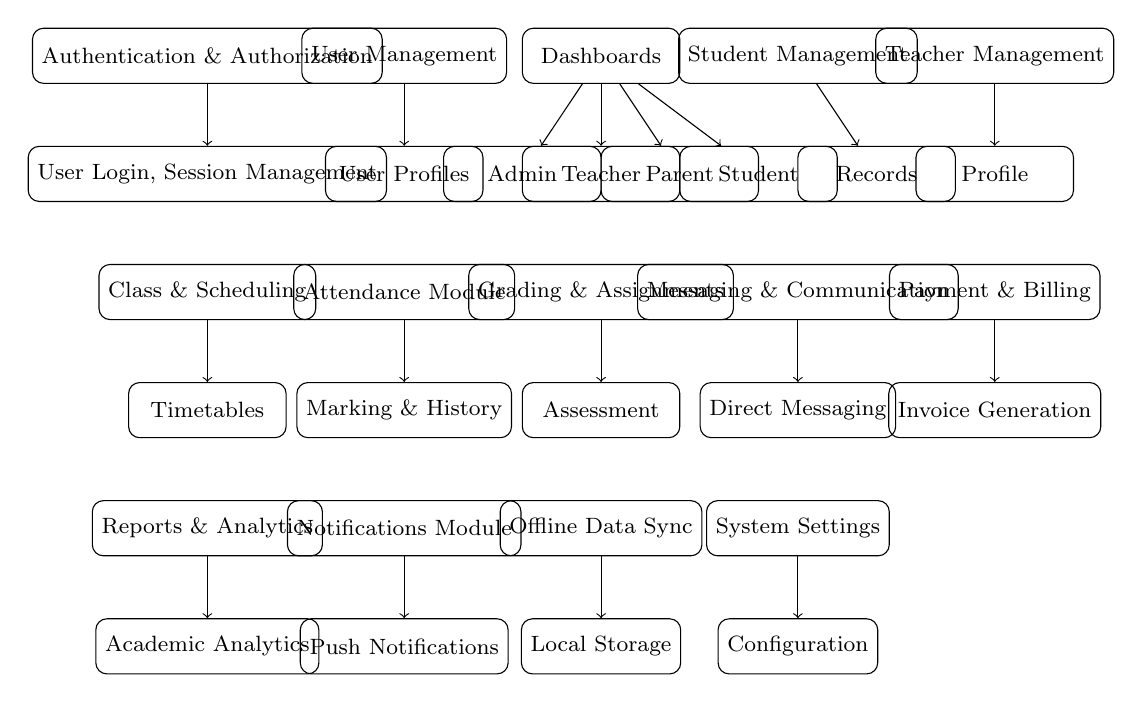
\begin{tikzpicture}[
  level 1/.style={sibling distance=20mm},
  level 2/.style={sibling distance=15mm},
  edge from parent/.style={draw,->},
  module/.style={rectangle, rounded corners, draw, align=center, minimum height=7mm, minimum width=20mm, font=\footnotesize}
]

% Top level modules
\node[module] (auth) at (0,0) {Authentication \& Authorization};
\node[module] (user) at (2.5,0) {User Management};
\node[module] (dash) at (5,0) {Dashboards};
\node[module] (student) at (7.5,0) {Student Management};
\node[module] (teacher) at (10,0) {Teacher Management};

% Second level modules
\node[module] (login) at (0,-1.5) {User Login, Session Management};
\node[module] (profiles) at (2.5,-1.5) {User Profiles};
\node[module] (admin) at (4,-1.5) {Admin};
\node[module] (teacherdash) at (5,-1.5) {Teacher};
\node[module] (parent) at (6,-1.5) {Parent};
\node[module] (studentdash) at (7,-1.5) {Student};
\node[module] (records) at (8.5,-1.5) {Records};
\node[module] (profile) at (10,-1.5) {Profile};

% Connect modules
\draw[->] (auth) -- (login);
\draw[->] (user) -- (profiles);
\draw[->] (dash) -- (admin);
\draw[->] (dash) -- (teacherdash);
\draw[->] (dash) -- (parent);
\draw[->] (dash) -- (studentdash);
\draw[->] (student) -- (records);
\draw[->] (teacher) -- (profile);

% Additional modules in next row
\node[module] (class) at (0,-3) {Class \& Scheduling};
\node[module] (attend) at (2.5,-3) {Attendance Module};
\node[module] (grade) at (5,-3) {Grading \& Assignments};
\node[module] (msg) at (7.5,-3) {Messaging \& Communication};
\node[module] (pay) at (10,-3) {Payment \& Billing};

% Connect additional modules
\node[module] (timetable) at (0,-4.5) {Timetables};
\node[module] (marking) at (2.5,-4.5) {Marking \& History};
\node[module] (assess) at (5,-4.5) {Assessment};
\node[module] (direct) at (7.5,-4.5) {Direct Messaging};
\node[module] (invoice) at (10,-4.5) {Invoice Generation};

\draw[->] (class) -- (timetable);
\draw[->] (attend) -- (marking);
\draw[->] (grade) -- (assess);
\draw[->] (msg) -- (direct);
\draw[->] (pay) -- (invoice);

% Final row of modules
\node[module] (report) at (0,-6) {Reports \& Analytics};
\node[module] (notif) at (2.5,-6) {Notifications Module};
\node[module] (offline) at (5,-6) {Offline Data Sync};
\node[module] (system) at (7.5,-6) {System Settings};

% Connect final row
\node[module] (analytics) at (0,-7.5) {Academic Analytics};
\node[module] (push) at (2.5,-7.5) {Push Notifications};
\node[module] (storage) at (5,-7.5) {Local Storage};
\node[module] (config) at (7.5,-7.5) {Configuration};

\draw[->] (report) -- (analytics);
\draw[->] (notif) -- (push);
\draw[->] (offline) -- (storage);
\draw[->] (system) -- (config);

\end{tikzpicture}
\caption{Comprehensive module structure of the school management system}
\label{fig:module_structure}
\end{figure}

\section{System Interaction Flow}

The following diagram illustrates how users interact with the system and how data flows between the various modules:

\begin{figure}[H]
\centering
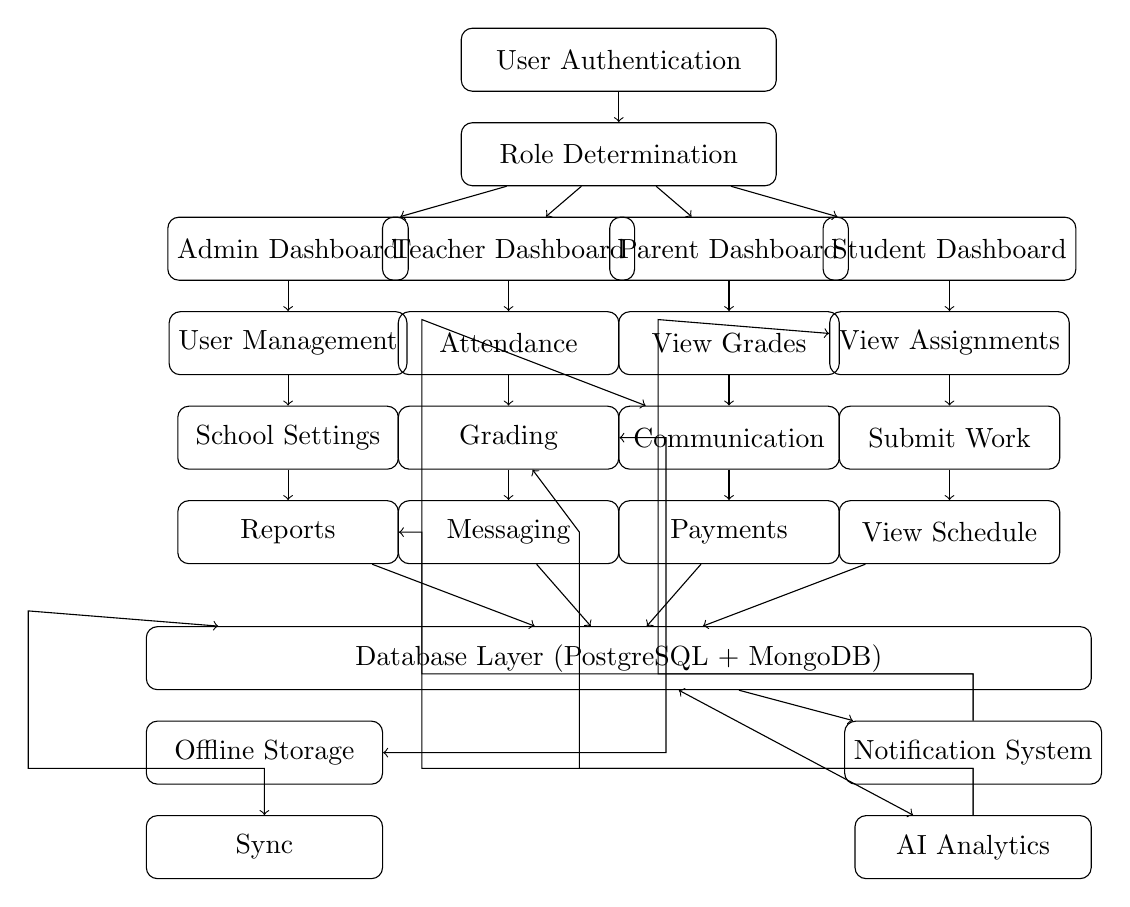
\begin{tikzpicture}[node distance=1.2cm, 
                    every node/.style={rectangle, rounded corners, draw, align=center, 
                                      minimum height=0.8cm}]

% Top row
\node[text centered, minimum width=4cm] (auth) {User Authentication};
\node[text centered, minimum width=4cm, below of=auth] (role) {Role Determination};

% Role-specific dashboards
\node[text centered, minimum width=2.8cm, below of=role, xshift=-4.2cm] (admin) {Admin Dashboard};
\node[text centered, minimum width=2.8cm, below of=role, xshift=-1.4cm] (teacher) {Teacher Dashboard};
\node[text centered, minimum width=2.8cm, below of=role, xshift=1.4cm] (parent) {Parent Dashboard};
\node[text centered, minimum width=2.8cm, below of=role, xshift=4.2cm] (student) {Student Dashboard};

% Action rows for each dashboard
\node[text centered, minimum width=2.8cm, below of=admin] (admin1) {User Management};
\node[text centered, minimum width=2.8cm, below of=admin1] (admin2) {School Settings};
\node[text centered, minimum width=2.8cm, below of=admin2] (admin3) {Reports};

\node[text centered, minimum width=2.8cm, below of=teacher] (teacher1) {Attendance};
\node[text centered, minimum width=2.8cm, below of=teacher1] (teacher2) {Grading};
\node[text centered, minimum width=2.8cm, below of=teacher2] (teacher3) {Messaging};

\node[text centered, minimum width=2.8cm, below of=parent] (parent1) {View Grades};
\node[text centered, minimum width=2.8cm, below of=parent1] (parent2) {Communication};
\node[text centered, minimum width=2.8cm, below of=parent2] (parent3) {Payments};

\node[text centered, minimum width=2.8cm, below of=student] (student1) {View Assignments};
\node[text centered, minimum width=2.8cm, below of=student1] (student2) {Submit Work};
\node[text centered, minimum width=2.8cm, below of=student2] (student3) {View Schedule};

% Database and supporting systems
\node[text centered, minimum width=12cm, below of=admin3, xshift=4.2cm, yshift=-0.4cm] (db) {Database Layer (PostgreSQL + MongoDB)};

\node[text centered, minimum width=3cm, below of=db, xshift=-4.5cm] (offline) {Offline Storage};
\node[text centered, minimum width=3cm, below of=offline] (sync) {Sync};

\node[text centered, minimum width=3cm, below of=db, xshift=4.5cm] (notif) {Notification System};
\node[text centered, minimum width=3cm, below of=notif] (ai) {AI Analytics};

% Connections
\draw[->] (auth) -- (role);
\draw[->] (role) -- (admin);
\draw[->] (role) -- (teacher);
\draw[->] (role) -- (parent);
\draw[->] (role) -- (student);

\draw[->] (admin) -- (admin1);
\draw[->] (admin1) -- (admin2);
\draw[->] (admin2) -- (admin3);

\draw[->] (teacher) -- (teacher1);
\draw[->] (teacher1) -- (teacher2);
\draw[->] (teacher2) -- (teacher3);

\draw[->] (parent) -- (parent1);
\draw[->] (parent1) -- (parent2);
\draw[->] (parent2) -- (parent3);

\draw[->] (student) -- (student1);
\draw[->] (student1) -- (student2);
\draw[->] (student2) -- (student3);

\draw[->] (admin3) -- (db);
\draw[->] (teacher3) -- (db);
\draw[->] (parent3) -- (db);
\draw[->] (student3) -- (db);

\draw[<->] (teacher2) -- ++(2,0) -- ++(0,-4) -- (offline);
\draw[->] (offline) -- (sync);
\draw[->] (sync) -- ++(0,1) -- ++(-3,0) -- ++(0,2) -- (db);

\draw[->] (db) -- (notif);
\draw[->] (notif) -- ++(0,1) -- ++(-7,0) -- ++(0,4.5) -- (parent2);
\draw[->] (notif) -- ++(0,1) -- ++(-4,0) -- ++(0,4.5) -- (student1);

\draw[<->] (db) -- (ai);
\draw[->] (ai) -- ++(0,1) -- ++(-7,0) -- ++(0,3) -- (admin3);
\draw[->] (ai) -- ++(0,1) -- ++(-5,0) -- ++(0,3) -- (teacher2);

\end{tikzpicture}
\caption{System interaction flow showing user roles, actions, and data processing}
\label{fig:system_interaction}
\end{figure}

\chapter{Implementation Roadmap}

\section{Phased Implementation Strategy}

To ensure rapid adoption and early value delivery, we recommend a phased implementation approach. This strategy allows for quick deployment of core functionality while gradually introducing more advanced features.

\begin{figure}[H]
\centering
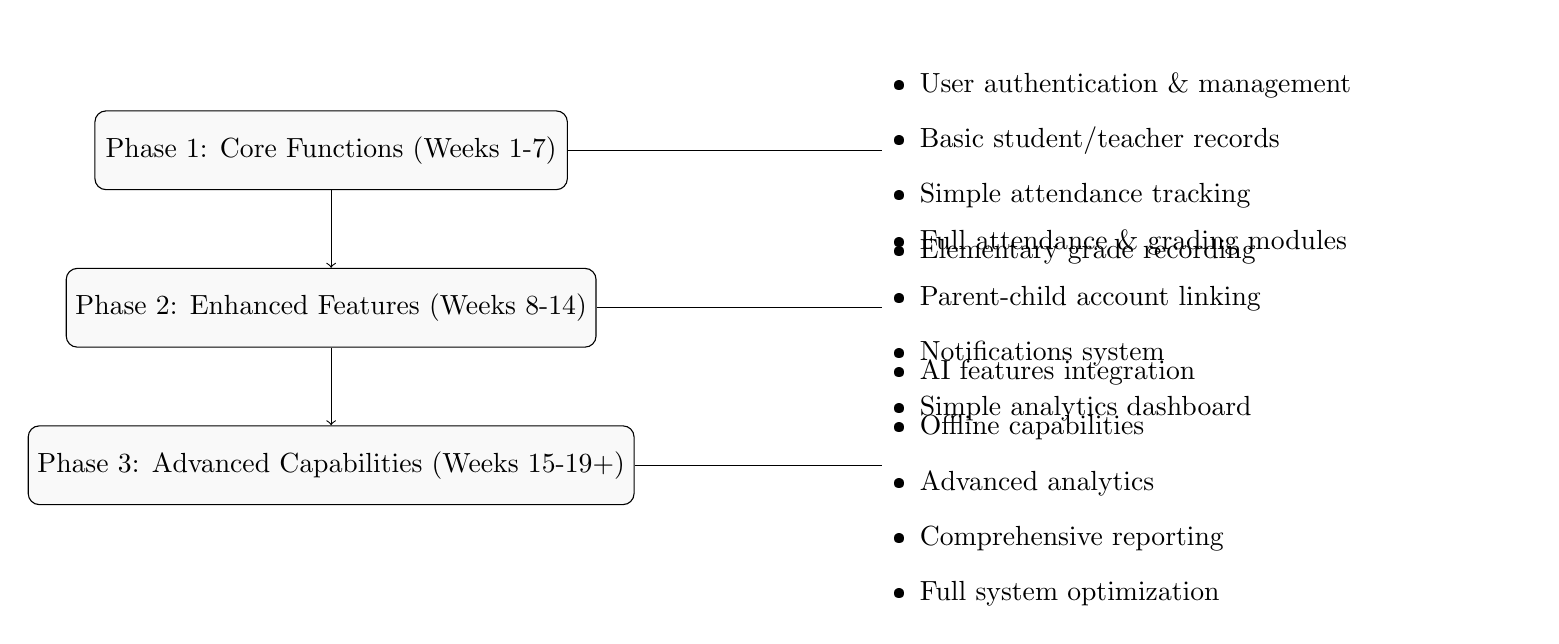
\begin{tikzpicture}[node distance=0.5cm, box/.style={rectangle, draw, rounded corners, minimum width=6cm, minimum height=1cm, text centered, fill=gray!5}]

\node[box] (phase1) at (0,0) {Phase 1: Core Functions (Weeks 1-7)};
\node[box] (phase2) at (0,-2) {Phase 2: Enhanced Features (Weeks 8-14)};
\node[box] (phase3) at (0,-4) {Phase 3: Advanced Capabilities (Weeks 15-19+)};

\node[text width=8cm, anchor=west] (phase1_details) at (7,0) {
\begin{itemize}[leftmargin=*]
\item User authentication \& management
\item Basic student/teacher records
\item Simple attendance tracking
\item Elementary grade recording
\end{itemize}
};

\node[text width=8cm, anchor=west] (phase2_details) at (7,-2) {
\begin{itemize}[leftmargin=*]
\item Full attendance \& grading modules
\item Parent-child account linking
\item Notifications system
\item Simple analytics dashboard
\end{itemize}
};

\node[text width=8cm, anchor=west] (phase3_details) at (7,-4) {
\begin{itemize}[leftmargin=*]
\item AI features integration
\item Offline capabilities
\item Advanced analytics
\item Comprehensive reporting
\item Full system optimization
\end{itemize}
};

\draw[->] (phase1) -- (phase2);
\draw[->] (phase2) -- (phase3);

\draw[-] (phase1.east) -- ++(1,0) -- (phase1_details.west);
\draw[-] (phase2.east) -- ++(1,0) -- (phase2_details.west);
\draw[-] (phase3.east) -- ++(1,0) -- (phase3_details.west);

\end{tikzpicture}
\caption{Phased implementation approach for the school management system}
\label{fig:phased_implementation}
\end{figure}

\section{Initial MVP Implementation}

The initial Minimum Viable Product (MVP) focuses on quickly delivering core functionality that provides immediate value to schools:

\begin{table}[H]
\centering
\begin{tabular}{|p{3.5cm}|p{9cm}|}
\hline
\textbf{Component} & \textbf{MVP Scope} \\
\hline
Authentication & Basic login/logout with role-based access for admins and teachers only \\
\hline
User Management & Manual creation of admin and teacher accounts; bulk upload of student records \\
\hline
Dashboards & Simple dashboards for admin and teacher access \\
\hline
Student Records & Basic student information management; class assignments \\
\hline
Attendance & Simple attendance marking interface with online-only functionality \\
\hline
Grading & Basic grade entry and simple report cards \\
\hline
Database & PostgreSQL implementation only (MongoDB integration deferred) \\
\hline
Deployment & Single-environment Azure deployment with manual scaling \\
\hline
\end{tabular}
\caption{Initial MVP scope for rapid implementation}
\end{table}

\section{Detailed Phase Roadmap}

\subsection{Phase 1: Requirements \& Design (Weeks 1-2)}
\begin{itemize}
    \item Gather detailed requirements from stakeholders
    \item Finalize feature set and refine architecture
    \item Choose specific technology components
    \item Set up project repository and structure
    \item Create detailed mockups for MVP user interfaces
\end{itemize}

\subsection{Phase 2: Initial Setup and CI/CD (Week 3)}
\begin{itemize}
    \item Initialize codebases for frontend and backend
    \item Set up development tools and code quality standards
    \item Establish CI/CD pipeline with GitHub Actions
    \item Create basic Azure development environment
    \item Set up basic project structure with module separation
\end{itemize}

\subsection{Phase 3: Core Backend Development (Weeks 4-6)}
\begin{itemize}
    \item Implement user management and authentication
    \item Set up database schemas and relationships
    \item Develop core API endpoints for basic functionality
    \item Configure role-based access control
    \item Implement bulk student upload functionality
\end{itemize}

\subsection{Phase 4: Core Frontend Development (Weeks 5-7)}
\begin{itemize}
    \item Build authentication UI and login flows
    \item Develop role-based dashboards
    \item Implement navigation and basic page structure
    \item Integrate with backend APIs
    \item Create MVP attendance and grading interfaces
\end{itemize}

\subsection{Phase 5: Feature Development (Weeks 8-11)}
\begin{itemize}
    \item Complete attendance management features with history and reporting
    \item Develop comprehensive grading and assessment modules
    \item Create notification system for important events
    \item Build basic reporting tools for administrators
    \item Implement parent-student account linking functionality
    \item Develop parent and student dashboards
\end{itemize}

\subsection{Phase 6: AI Features Integration (Weeks 12-14)}
\begin{itemize}
    \item Integrate Azure Cognitive Services for facial recognition attendance
    \item Develop analytics module for student performance insights
    \item Implement predictive modeling for identifying at-risk students
    \item Create AI-enhanced dashboards and visualizations
    \item Build intelligent reporting with trend analysis
\end{itemize}

\subsection{Phase 7: Offline Mode and PWA (Weeks 15-16)}
\begin{itemize}
    \item Implement service worker for asset caching
    \item Develop IndexedDB storage for offline data capture
    \item Create background sync mechanisms for attendance and grades
    \item Test and optimize offline workflows
    \item Implement PWA installation capabilities
\end{itemize}

\subsection{Phase 8: Testing \& Quality Assurance (Week 17)}
\begin{itemize}
    \item Conduct comprehensive testing (unit, integration, end-to-end)
    \item Perform security audits and vulnerability assessments
    \item Test performance under various conditions including poor connectivity
    \item Collect and incorporate user feedback
    \item Verify accessibility compliance
\end{itemize}

\subsection{Phase 9: Deployment \& Launch (Week 18)}
\begin{itemize}
    \item Finalize production environment on Azure
    \item Deploy application through CI/CD pipeline
    \item Conduct final validation testing
    \item Plan and execute phased rollout strategy
    \item Provide user training and documentation
\end{itemize}

\subsection{Phase 10: Post-Launch Support (Week 19+)}
\begin{itemize}
    \item Monitor system performance and user adoption
    \item Address any issues or bugs discovered
    \item Gather feedback for future improvements
    \item Plan next iteration of features
    \item Develop roadmap for additional modules (e.g., Payment & Billing)
\end{itemize}

\chapter{Technical Implementation Details}

\section{Initial MVP Implementation Details}

For the initial MVP launch (Phase 1), we will focus on implementing the following core components in a streamlined manner to ensure quick delivery of value:

\subsection{Core MVP Modules}
\begin{itemize}
    \item \textbf{Authentication:} Basic login/logout with JWT and role-based access
    \item \textbf{User Management:} Admin creation of users and bulk upload of students
    \item \textbf{Student Records:} Basic information management and class assignments
    \item \textbf{Attendance:} Simple online attendance tracking interface
    \item \textbf{Grading:} Basic grade entry and simple report cards
\end{itemize}

\begin{figure}[H]
\centering
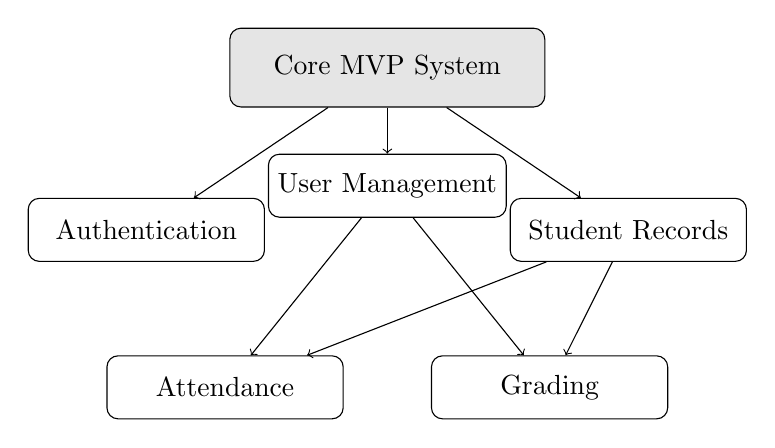
\begin{tikzpicture}[node distance=1.5cm]
\node (core) [rectangle, rounded corners, minimum width=4cm, minimum height=1cm, text centered, draw=black, fill=gray!20] {Core MVP System};

\node (auth) [rectangle, rounded corners, minimum width=3cm, minimum height=0.8cm, text centered, draw=black, below left of=core, xshift=-2cm, yshift=-1cm] {Authentication};
\node (users) [rectangle, rounded corners, minimum width=3cm, minimum height=0.8cm, text centered, draw=black, below of=core] {User Management};
\node (records) [rectangle, rounded corners, minimum width=3cm, minimum height=0.8cm, text centered, draw=black, below right of=core, xshift=2cm, yshift=-1cm] {Student Records};
\node (attend) [rectangle, rounded corners, minimum width=3cm, minimum height=0.8cm, text centered, draw=black, below left of=users, xshift=-1cm, yshift=-1.5cm] {Attendance};
\node (grade) [rectangle, rounded corners, minimum width=3cm, minimum height=0.8cm, text centered, draw=black, below right of=users, xshift=1cm, yshift=-1.5cm] {Grading};

\draw[->] (core) -- (auth);
\draw[->] (core) -- (users);
\draw[->] (core) -- (records);
\draw[->] (users) -- (attend);
\draw[->] (users) -- (grade);
\draw[->] (records) -- (attend);
\draw[->] (records) -- (grade);

\end{tikzpicture}
\caption{Initial MVP module relationships}
\end{figure}

\subsection{MVP Database Schema}
For the MVP, we will implement a simplified database schema focusing on essential tables:

\begin{figure}[H]
\centering
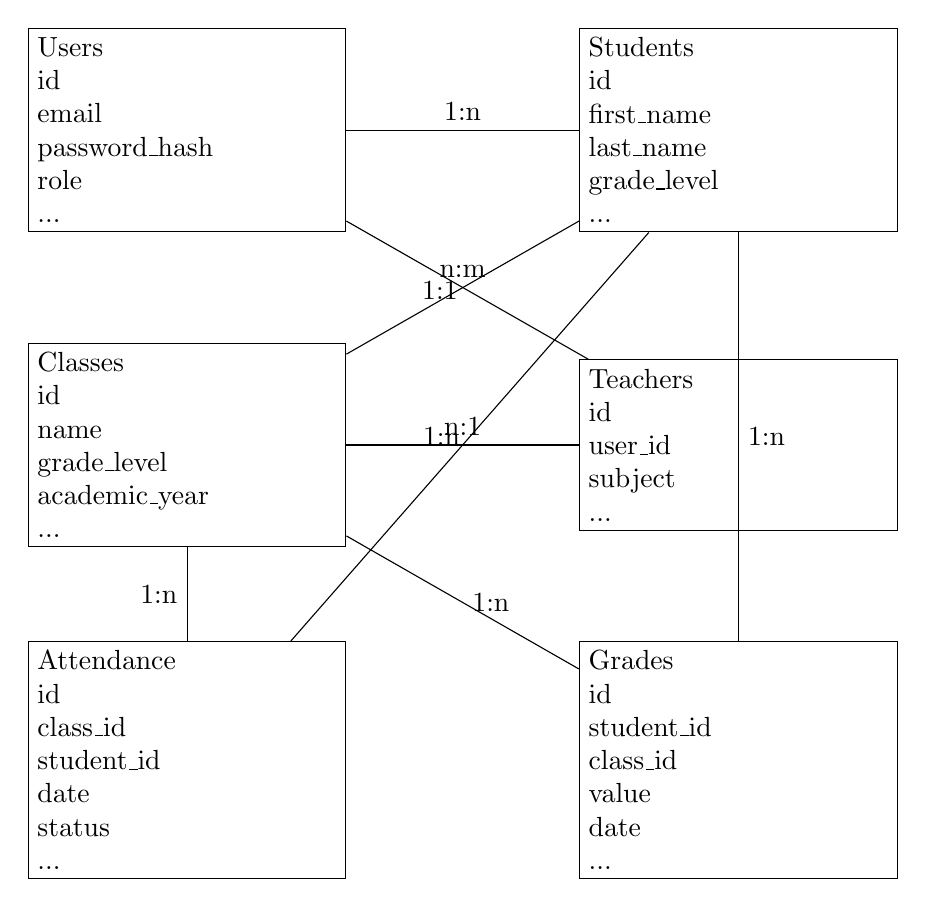
\begin{tikzpicture}[
  entity/.style={rectangle,draw,minimum width=4cm,minimum height=1.5cm,text width=3.8cm},
  relationship/.style={diamond,draw,minimum width=2.5cm,minimum height=1.5cm,text width=2.3cm,align=center},
  line/.style={-}
]

\node[entity] (users) at (0,0) {Users\\id\\email\\password\_hash\\role\\...};
\node[entity] (students) at (7,0) {Students\\id\\first\_name\\last\_name\\grade\_level\\...};
\node[entity] (classes) at (0,-4) {Classes\\id\\name\\grade\_level\\academic\_year\\...};
\node[entity] (teachers) at (7,-4) {Teachers\\id\\user\_id\\subject\\...};
\node[entity] (attendance) at (0,-8) {Attendance\\id\\class\_id\\student\_id\\date\\status\\...};
\node[entity] (grades) at (7,-8) {Grades\\id\\student\_id\\class\_id\\value\\date\\...};

\draw[line] (users) -- (students) node[midway,above] {1:n};
\draw[line] (users) -- (teachers) node[midway,left] {1:1};
\draw[line] (classes) -- (teachers) node[midway,above] {n:1};
\draw[line] (classes) -- (students) node[midway,above] {n:m};
\draw[line] (students) -- (attendance) node[midway,left] {1:n};
\draw[line] (classes) -- (attendance) node[midway,left] {1:n};
\draw[line] (students) -- (grades) node[midway,right] {1:n};
\draw[line] (classes) -- (grades) node[midway,right] {1:n};

\end{tikzpicture}
\caption{MVP database entity relationship diagram}
\end{figure}

\section{Frontend Technical Stack}

\subsection{Core Technologies}
\begin{itemize}
    \item \textbf{React:} Main library for UI development
    \item \textbf{Next.js:} Framework for server-side rendering and routing
    \item \textbf{TypeScript:} For type safety and improved developer experience
    \item \textbf{Material-UI:} Component library for consistent design
    \item \textbf{React Query:} For efficient data fetching and caching
    \item \textbf{React Context API:} For state management
    \item \textbf{Workbox:} For service worker implementation
\end{itemize}

\subsection{Frontend Organization}
The React application will follow this structure:
\begin{verbatim}
/src
  /components           # Reusable UI components
    /common             # Shared components (buttons, inputs, etc.)
    /layout             # Layout components (header, sidebar, etc.)
    /forms              # Form components
    /dashboards         # Dashboard components per role
  /hooks                # Custom React hooks
  /context              # Context providers
  /services             # API service calls
  /utils                # Utility functions
  /pages                # Next.js pages/routes
  /styles               # Global styles and themes
  /public               # Static assets
    /manifest.json      # PWA manifest
    /service-worker.js  # Service worker for offline capabilities
\end{verbatim}

\section{Backend Technical Stack}

\subsection{Core Technologies}
\begin{itemize}
    \item \textbf{Node.js:} Runtime environment
    \item \textbf{NestJS:} Backend framework
    \item \textbf{TypeScript:} For type safety
    \item \textbf{TypeORM/Prisma:} ORM for database interactions
    \item \textbf{Passport:} Authentication middleware
    \item \textbf{JWT:} For secure token-based authentication
    \item \textbf{Class-validator:} For input validation
\end{itemize}

\subsection{Backend Organization}
The NestJS application will follow this modular structure:
\begin{verbatim}
/src
  /main.ts              # Application entry point
  /app.module.ts        # Root module
  /auth                 # Authentication module
    /controllers        # Auth endpoints
    /services           # Auth business logic
    /\section{Parent Communication Workflow}

\begin{figure}[H]
\centering
\resizebox{\textwidth}{!}{
\begin{tikzpicture}[node distance=2.5cm]
\node (login) [rectangle, rounded corners, minimum width=4cm, minimum height=0.8cm, text centered, draw=black] {Parent logs into system};

\node (dashboard) [rectangle, rounded corners, minimum width=4cm, minimum height=0.8cm, text centered, draw=black, below of=login] {Parent views dashboard};

\node (child) [rectangle, rounded corners, minimum width=4cm, minimum height=0.8cm, text centered, draw=black, below of=dashboard] {Parent selects child (if multiple)};

\node (decision) [diamond, minimum width=3.5cm, minimum height=1.8cm, text centered, draw=black, below of=child, yshift=-1.2cm] {Communication\\ Type?};

\node (teacher) [rectangle, rounded corners, minimum width=4cm, minimum height=0.8cm, text centered, draw=black, below of=decision, xshift=-5cm, yshift=-1.2cm] {Message Teacher};

\node (admin) [rectangle, rounded corners, minimum width=4cm, minimum height=0.8cm, text centered, draw=black, below of=decision, xshift=5cm, yshift=-1.2cm] {Contact Administration};

\node (compose) [rectangle, rounded corners, minimum width=4cm, minimum height=0.8cm, text centered, draw=black, below of=teacher, yshift=-0.8cm] {Compose message};

\node (admin_form) [rectangle, rounded corners, minimum width=4cm, minimum height=0.8cm, text centered, draw=black, below of=admin, yshift=-0.8cm] {Fill contact form};

\node (topics) [rectangle, rounded corners, minimum width=5cm, minimum height=1.5cm, text centered, draw=black, below of=compose, yshift=-0.8cm] {- Attendance issues\\ - Academic performance\\ - Assignment clarifications};

\node (admin_topics) [rectangle, rounded corners, minimum width=5cm, minimum height=1.5cm, text centered, draw=black, below of=admin_form, yshift=-0.8cm] {- Administrative requests\\ - Account issues\\ - General feedback};

\node (follow_up) [rectangle, rounded corners, minimum width=6cm, minimum height=0.8cm, text centered, draw=black, below of=topics, xshift=2.5cm, yshift=-2cm] {Parent receives notification when response arrives};

\node (history) [rectangle, rounded corners, minimum width=6cm, minimum height=0.8cm, text centered, draw=black, below of=follow_up, yshift=-0.8cm] {Communication history available for reference};

\draw[->] (login) -- (dashboard);
\draw[->] (dashboard) -- (child);
\draw[->] (child) -- (decision);
\draw[->] (decision) -- (teacher) node[midway, above, sloped] {Teacher};
\draw[->] (decision) -- (admin) node[midway, above, sloped] {Administration};
\draw[->] (teacher) -- (compose);
\draw[->] (admin) -- (admin_form);
\draw[->] (compose) -- (topics);
\draw[->] (admin_form) -- (admin_topics);
\draw[->] (topics) |- (follow_up);
\draw[->] (admin_topics) |- (follow_up);
\draw[->] (follow_up) -- (history);
\end{tikzpicture}
}
\caption{Parent communication workflow}
\end{figure}

\section{Key Implementation Challenges \& Mitigation Strategies}

During the implementation of the school management system, several technical and organizational challenges are anticipated. This section outlines these challenges and provides strategies to address them effectively.

\subsection{Technical Challenges}

\begin{table}[H]
\centering
\begin{tabular}{|p{3.5cm}|p{5.5cm}|p{5.5cm}|}
\hline
\textbf{Challenge} & \textbf{Description} & \textbf{Mitigation Strategy} \\
\hline
Data Migration & Transferring existing student, teacher, and academic records from legacy systems & \begin{itemize}
\item Develop specialized ETL scripts
\item Implement a phased migration approach
\item Provide a transitional period with both systems
\end{itemize} \\
\hline
Offline Reliability & Ensuring data integrity during offline usage and synchronization & \begin{itemize}
\item Robust conflict resolution mechanisms
\item Clear timestamp-based precedence rules
\item Comprehensive sync status indicators
\end{itemize} \\
\hline
Performance at Scale & Maintaining responsive performance with large datasets and concurrent users & \begin{itemize}
\item Implement database indexing strategies
\item Use caching for frequently accessed data
\item Design for horizontal scalability on Azure
\end{itemize} \\
\hline
AI Model Accuracy & Building accurate prediction and facial recognition models & \begin{itemize}
\item Start with conservative, high-confidence predictions
\item Continuously improve models with new data
\item Provide manual override options
\end{itemize} \\
\hline
Security & Protecting sensitive student data and preventing unauthorized access & \begin{itemize}
\item Regular security audits and penetration testing
\item End-to-end encryption for sensitive data
\item Comprehensive role-based access controls
\end{itemize} \\
\hline
\end{tabular}
\caption{Technical implementation challenges and mitigation strategies}
\end{table}

\subsection{Organizational Challenges}

\begin{table}[H]
\centering
\begin{tabular}{|p{3.5cm}|p{5.5cm}|p{5.5cm}|}
\hline
\textbf{Challenge} & \textbf{Description} & \textbf{Mitigation Strategy} \\
\hline
User Adoption & Ensuring stakeholders embrace and effectively use the new system & \begin{itemize}
\item Comprehensive training program
\item Intuitive UX design for minimal learning curve
\item Designated "super users" within each user group
\end{itemize} \\
\hline
Changing Requirements & Managing evolving requirements during implementation & \begin{itemize}
\item Agile methodology for adaptability
\item Regular stakeholder feedback sessions
\item Modular design for feature flexibility
\end{itemize} \\
\hline
Training & Educating staff, parents, and students on system usage & \begin{itemize}
\item Role-specific training materials and videos
\item In-app guided tours and contextual help
\item Support desk during initial deployment
\end{itemize} \\
\hline
Workflow Integration & Adapting the system to existing school processes & \begin{itemize}
\item Process mapping workshops before implementation
\item Configurable workflows in the system
\item Phased approach to process changes
\end{itemize} \\
\hline
Stakeholder Alignment & Managing expectations across diverse stakeholder groups & \begin{itemize}
\item Regular progress updates and demos
\item Clear communication about features and limitations
\item Feedback channels for continuous improvement
\end{itemize} \\
\hline
\end{tabular}
\caption{Organizational implementation challenges and mitigation strategies}
\end{table}

\chapter{Data Security \& Compliance}

Protecting sensitive student and academic data is a critical aspect of the school management system implementation. This section outlines the comprehensive security measures and compliance considerations incorporated into the design.

\section{Security Architecture}

\begin{figure}[H]
\centering
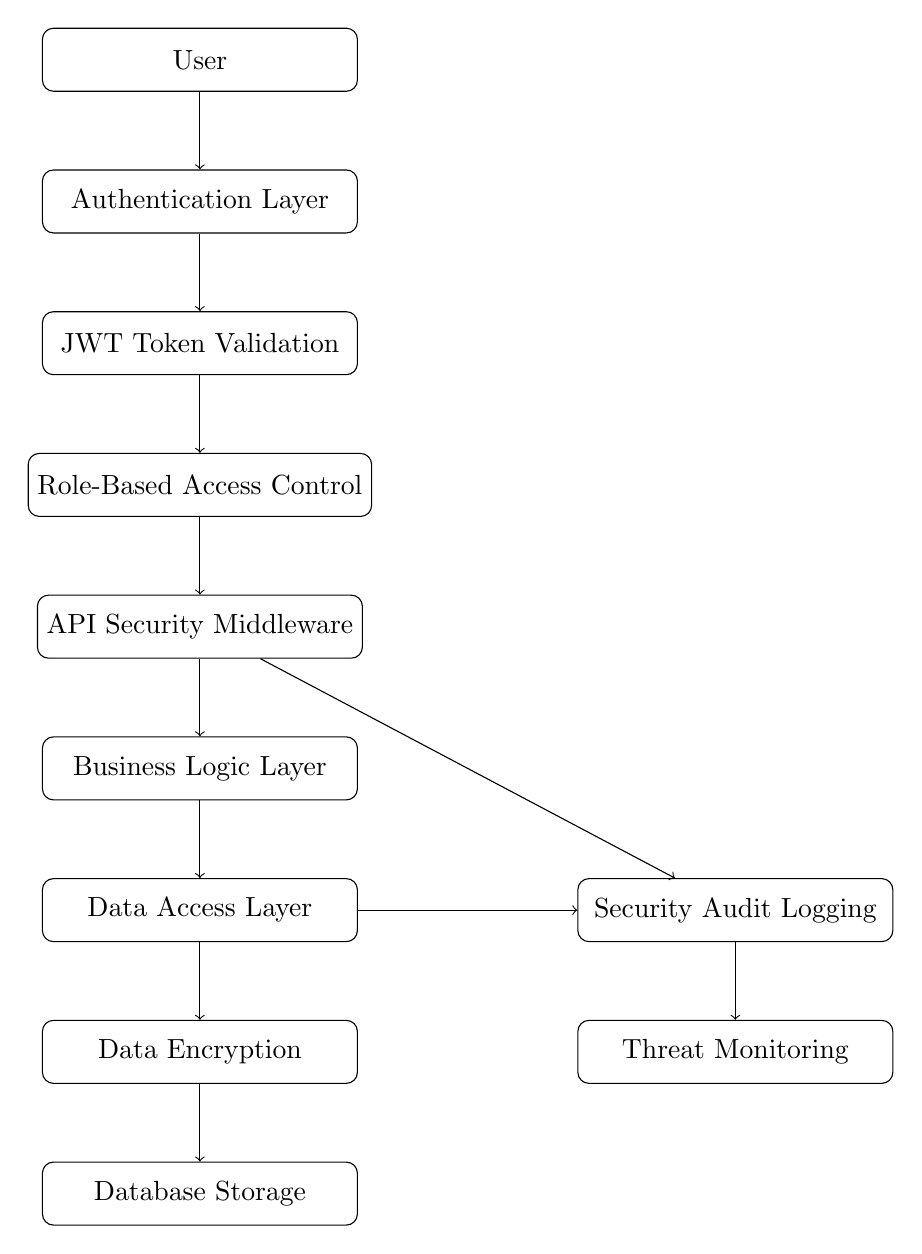
\begin{tikzpicture}[node distance=1.8cm]
\node (user) [rectangle, rounded corners, minimum width=4cm, minimum height=0.8cm, text centered, draw=black] {User};

\node (auth) [rectangle, rounded corners, minimum width=4cm, minimum height=0.8cm, text centered, draw=black, below of=user] {Authentication Layer};

\node (jwt) [rectangle, rounded corners, minimum width=4cm, minimum height=0.8cm, text centered, draw=black, below of=auth] {JWT Token Validation};

\node (rbac) [rectangle, rounded corners, minimum width=4cm, minimum height=0.8cm, text centered, draw=black, below of=jwt] {Role-Based Access Control};

\node (api) [rectangle, rounded corners, minimum width=4cm, minimum height=0.8cm, text centered, draw=black, below of=rbac] {API Security Middleware};

\node (business) [rectangle, rounded corners, minimum width=4cm, minimum height=0.8cm, text centered, draw=black, below of=api] {Business Logic Layer};

\node (data) [rectangle, rounded corners, minimum width=4cm, minimum height=0.8cm, text centered, draw=black, below of=business] {Data Access Layer};

\node (encryption) [rectangle, rounded corners, minimum width=4cm, minimum height=0.8cm, text centered, draw=black, below of=data] {Data Encryption};

\node (database) [rectangle, rounded corners, minimum width=4cm, minimum height=0.8cm, text centered, draw=black, below of=encryption] {Database Storage};

\node (logging) [rectangle, rounded corners, minimum width=4cm, minimum height=0.8cm, text centered, draw=black, right of=data, xshift=5cm] {Security Audit Logging};

\node (monitoring) [rectangle, rounded corners, minimum width=4cm, minimum height=0.8cm, text centered, draw=black, below of=logging] {Threat Monitoring};

\draw[->] (user) -- (auth);
\draw[->] (auth) -- (jwt);
\draw[->] (jwt) -- (rbac);
\draw[->] (rbac) -- (api);
\draw[->] (api) -- (business);
\draw[->] (business) -- (data);
\draw[->] (data) -- (encryption);
\draw[->] (encryption) -- (database);
\draw[->] (api) -- (logging);
\draw[->] (data) -- (logging);
\draw[->] (logging) -- (monitoring);

\end{tikzpicture}
\caption{Security architecture of the school management system}
\end{figure}

\section{Security Measures}

\begin{itemize}
    \item \textbf{Authentication:} Multi-factor authentication for administrative accounts, strong password policies, and secure password reset mechanisms.
    
    \item \textbf{Authorization:} Granular role-based access control ensuring users only access data appropriate to their role.
    
    \item \textbf{Data Encryption:} All sensitive data encrypted both in transit (HTTPS/TLS) and at rest (AES-256 encryption).
    
    \item \textbf{Secure APIs:} API endpoints protected against common vulnerabilities (injection, XSS, CSRF) with input validation and sanitization.
    
    \item \textbf{Audit Logging:} Comprehensive logging of all security-relevant events and access to sensitive data.
    
    \item \textbf{Regular Security Testing:} Scheduled penetration testing and vulnerability assessments.
    
    \item \textbf{Secure Development:} Following secure coding practices and regular dependency vulnerability scanning.
    
    \item \textbf{Data Minimization:} Collecting and storing only necessary data to reduce exposure risk.
\end{itemize}

\section{Compliance Considerations}

\begin{table}[H]
\centering
\begin{tabular}{|p{3cm}|p{11.5cm}|}
\hline
\textbf{Regulation} & \textbf{Implementation Approach} \\
\hline
FERPA (USA) & \begin{itemize}
\item Parental consent for sharing student information
\item Audit trails for all data access
\item Strict access controls limiting data visibility
\item Ability to generate compliance reports
\end{itemize} \\
\hline
GDPR (EU) & \begin{itemize}
\item Data processing consent management
\item Right to access, rectification, and erasure mechanisms
\item Data breach notification capabilities
\item Data retention policies and automated purging
\end{itemize} \\
\hline
COPPA (USA) & \begin{itemize}
\item Age verification for student accounts
\item Parental consent management
\item Limited data collection from minors
\item Simplified privacy notices
\end{itemize} \\
\hline
Local Education Laws & \begin{itemize}
\item Configurable data retention policies
\item Compliance reporting capabilities
\item Adaptable privacy controls for regional requirements
\end{itemize} \\
\hline
\end{tabular}
\caption{Compliance considerations and implementation approaches}
\end{table}

\chapter{Training \& Adoption Strategy}

A comprehensive training and adoption strategy is essential for successful implementation of the school management system. This section outlines the approach to ensure all stakeholders can effectively use the system.

\section{Training Approach}

\begin{figure}[H]
\centering
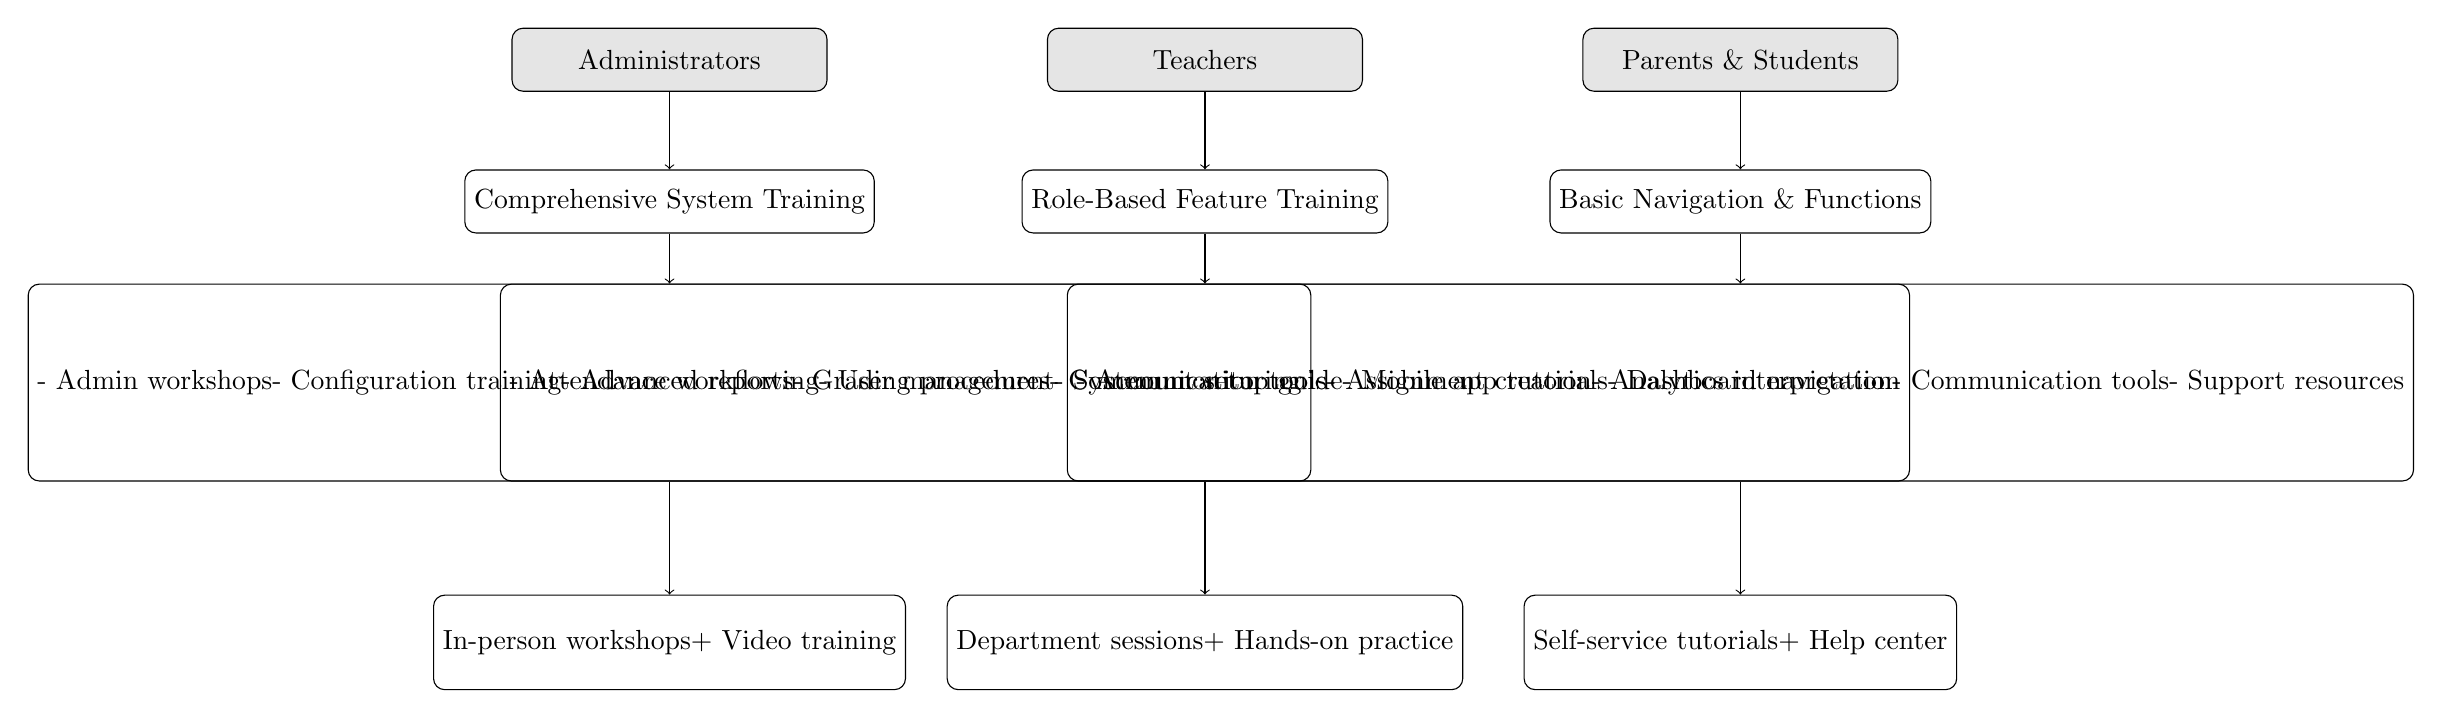
\begin{tikzpicture}[node distance=1.8cm]
\node (admin) [rectangle, rounded corners, minimum width=4cm, minimum height=0.8cm, text centered, draw=black, fill=gray!20] {Administrators};
\node (teacher) [rectangle, rounded corners, minimum width=4cm, minimum height=0.8cm, text centered, draw=black, fill=gray!20, right of=admin, xshift=5cm] {Teachers};
\node (parent) [rectangle, rounded corners, minimum width=4cm, minimum height=0.8cm, text centered, draw=black, fill=gray!20, right of=teacher, xshift=5cm] {Parents \& Students};

\node (training1) [rectangle, rounded corners, minimum width=4cm, minimum height=0.8cm, text centered, draw=black, below of=admin] {Comprehensive System Training};
\node (training2) [rectangle, rounded corners, minimum width=4cm, minimum height=0.8cm, text centered, draw=black, below of=teacher] {Role-Based Feature Training};
\node (training3) [rectangle, rounded corners, minimum width=4cm, minimum height=0.8cm, text centered, draw=black, below of=parent] {Basic Navigation \& Functions};

\node (material1) [rectangle, rounded corners, minimum width=4cm, minimum height=2.5cm, text centered, draw=black, below of=training1, yshift=-0.5cm] {- Admin workshops\\ - Configuration training\\ - Advanced reporting\\ - User management\\ - System monitoring};
\node (material2) [rectangle, rounded corners, minimum width=4cm, minimum height=2.5cm, text centered, draw=black, below of=training2, yshift=-0.5cm] {- Attendance workflows\\ - Grading procedures\\ - Communication tools\\ - Assignment creation\\ - Analytics interpretation};
\node (material3) [rectangle, rounded corners, minimum width=4cm, minimum height=2.5cm, text centered, draw=black, below of=training3, yshift=-0.5cm] {- Account setup guide\\ - Mobile app tutorials\\ - Dashboard navigation\\ - Communication tools\\ - Support resources};

\node (delivery1) [rectangle, rounded corners, minimum width=4cm, minimum height=1.2cm, text centered, draw=black, below of=material1, yshift=-1.5cm] {In-person workshops\\ + Video training};
\node (delivery2) [rectangle, rounded corners, minimum width=4cm, minimum height=1.2cm, text centered, draw=black, below of=material2, yshift=-1.5cm] {Department sessions\\ + Hands-on practice};
\node (delivery3) [rectangle, rounded corners, minimum width=4cm, minimum height=1.2cm, text centered, draw=black, below of=material3, yshift=-1.5cm] {Self-service tutorials\\ + Help center};

\draw[->] (admin) -- (training1);
\draw[->] (teacher) -- (training2);
\draw[->] (parent) -- (training3);
\draw[->] (training1) -- (material1);
\draw[->] (training2) -- (material2);
\draw[->] (training3) -- (material3);
\draw[->] (material1) -- (delivery1);
\draw[->] (material2) -- (delivery2);
\draw[->] (material3) -- (delivery3);

\end{tikzpicture}
\caption{Role-based training approach}
\end{figure}

\section{Training Materials}

\begin{itemize}
    \item \textbf{Documentation:} Comprehensive user manuals, quick reference guides, and FAQ documents.
    
    \item \textbf{Video Tutorials:} Role-specific video tutorials demonstrating key system functions.
    
    \item \textbf{Interactive Guides:} In-app walkthroughs and tooltips for key features.
    
    \item \textbf{Training Environments:} Sandbox environments for practice without affecting production data.
    
    \item \textbf{Webinars:} Live and recorded training sessions for different user roles.
    
    \item \textbf{Knowledge Base:} Searchable library of how-to articles and troubleshooting guides.
\end{itemize}

\section{Adoption Strategy}

\begin{figure}[H]
\centering
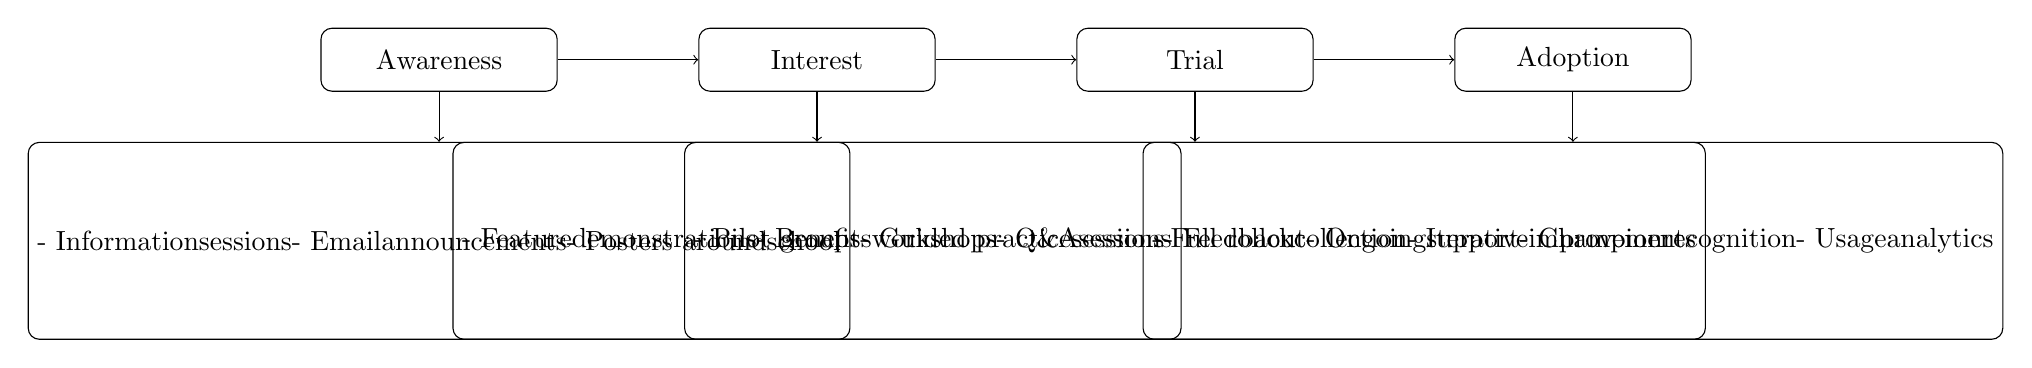
\begin{tikzpicture}[node distance=1.8cm]

\node (awareness) [rectangle, rounded corners, minimum width=3cm, minimum height=0.8cm, text centered, draw=black] {Awareness};
\node (interest) [rectangle, rounded corners, minimum width=3cm, minimum height=0.8cm, text centered, draw=black, right of=awareness, xshift=3cm] {Interest};
\node (trial) [rectangle, rounded corners, minimum width=3cm, minimum height=0.8cm, text centered, draw=black, right of=interest, xshift=3cm] {Trial};
\node (adoption) [rectangle, rounded corners, minimum width=3cm, minimum height=0.8cm, text centered, draw=black, right of=trial, xshift=3cm] {Adoption};

\node (activity1) [rectangle, rounded corners, minimum width=3cm, minimum height=2.5cm, text centered, draw=black, below of=awareness, yshift=-0.5cm] {- Information\\ sessions\\ - Email\\ announcements\\ - Posters around\\ school};
\node (activity2) [rectangle, rounded corners, minimum width=3cm, minimum height=2.5cm, text centered, draw=black, below of=interest, yshift=-0.5cm] {- Feature\\ demonstrations\\ - Benefits\\ workshops\\ - Q\&A\\ sessions};
\node (activity3) [rectangle, rounded corners, minimum width=3cm, minimum height=2.5cm, text centered, draw=black, below of=trial, yshift=-0.5cm] {- Pilot groups\\ - Guided practice\\ sessions\\ - Feedback\\ collection\\ - Iterative\\ improvements};
\node (activity4) [rectangle, rounded corners, minimum width=3cm, minimum height=2.5cm, text centered, draw=black, below of=adoption, yshift=-0.5cm] {- Full rollout\\ - Ongoing\\ support\\ - Champion\\ recognition\\ - Usage\\ analytics};

\draw[->] (awareness) -- (interest);
\draw[->] (interest) -- (trial);
\draw[->] (trial) -- (adoption);
\draw[->] (awareness) -- (activity1);
\draw[->] (interest) -- (activity2);
\draw[->] (trial) -- (activity3);
\draw[->] (adoption) -- (activity4);

\end{tikzpicture}
\caption{Phased adoption strategy}
\end{figure}

\section{Support Infrastructure}

\begin{itemize}
    \item \textbf{Help Desk:} Dedicated support team available during implementation and early adoption phases.
    
    \item \textbf{Super Users:} Identified power users within each stakeholder group who receive advanced training and act as first-line support.
    
    \item \textbf{Feedback Mechanisms:} In-app feedback tools and regular surveys to identify usability issues or training gaps.
    
    \item \textbf{Support Tiers:} Structured escalation process from basic troubleshooting to advanced technical support.
    
    \item \textbf{Usage Analytics:} Monitoring of system usage patterns to identify features requiring additional training.
\end{itemize}

\chapter{System Integrations}

The school management system is designed to integrate with existing school technology infrastructure and third-party educational systems to create a comprehensive ecosystem.

\section{Integration Architecture}

\begin{landscape}
\begin{figure}
\centering
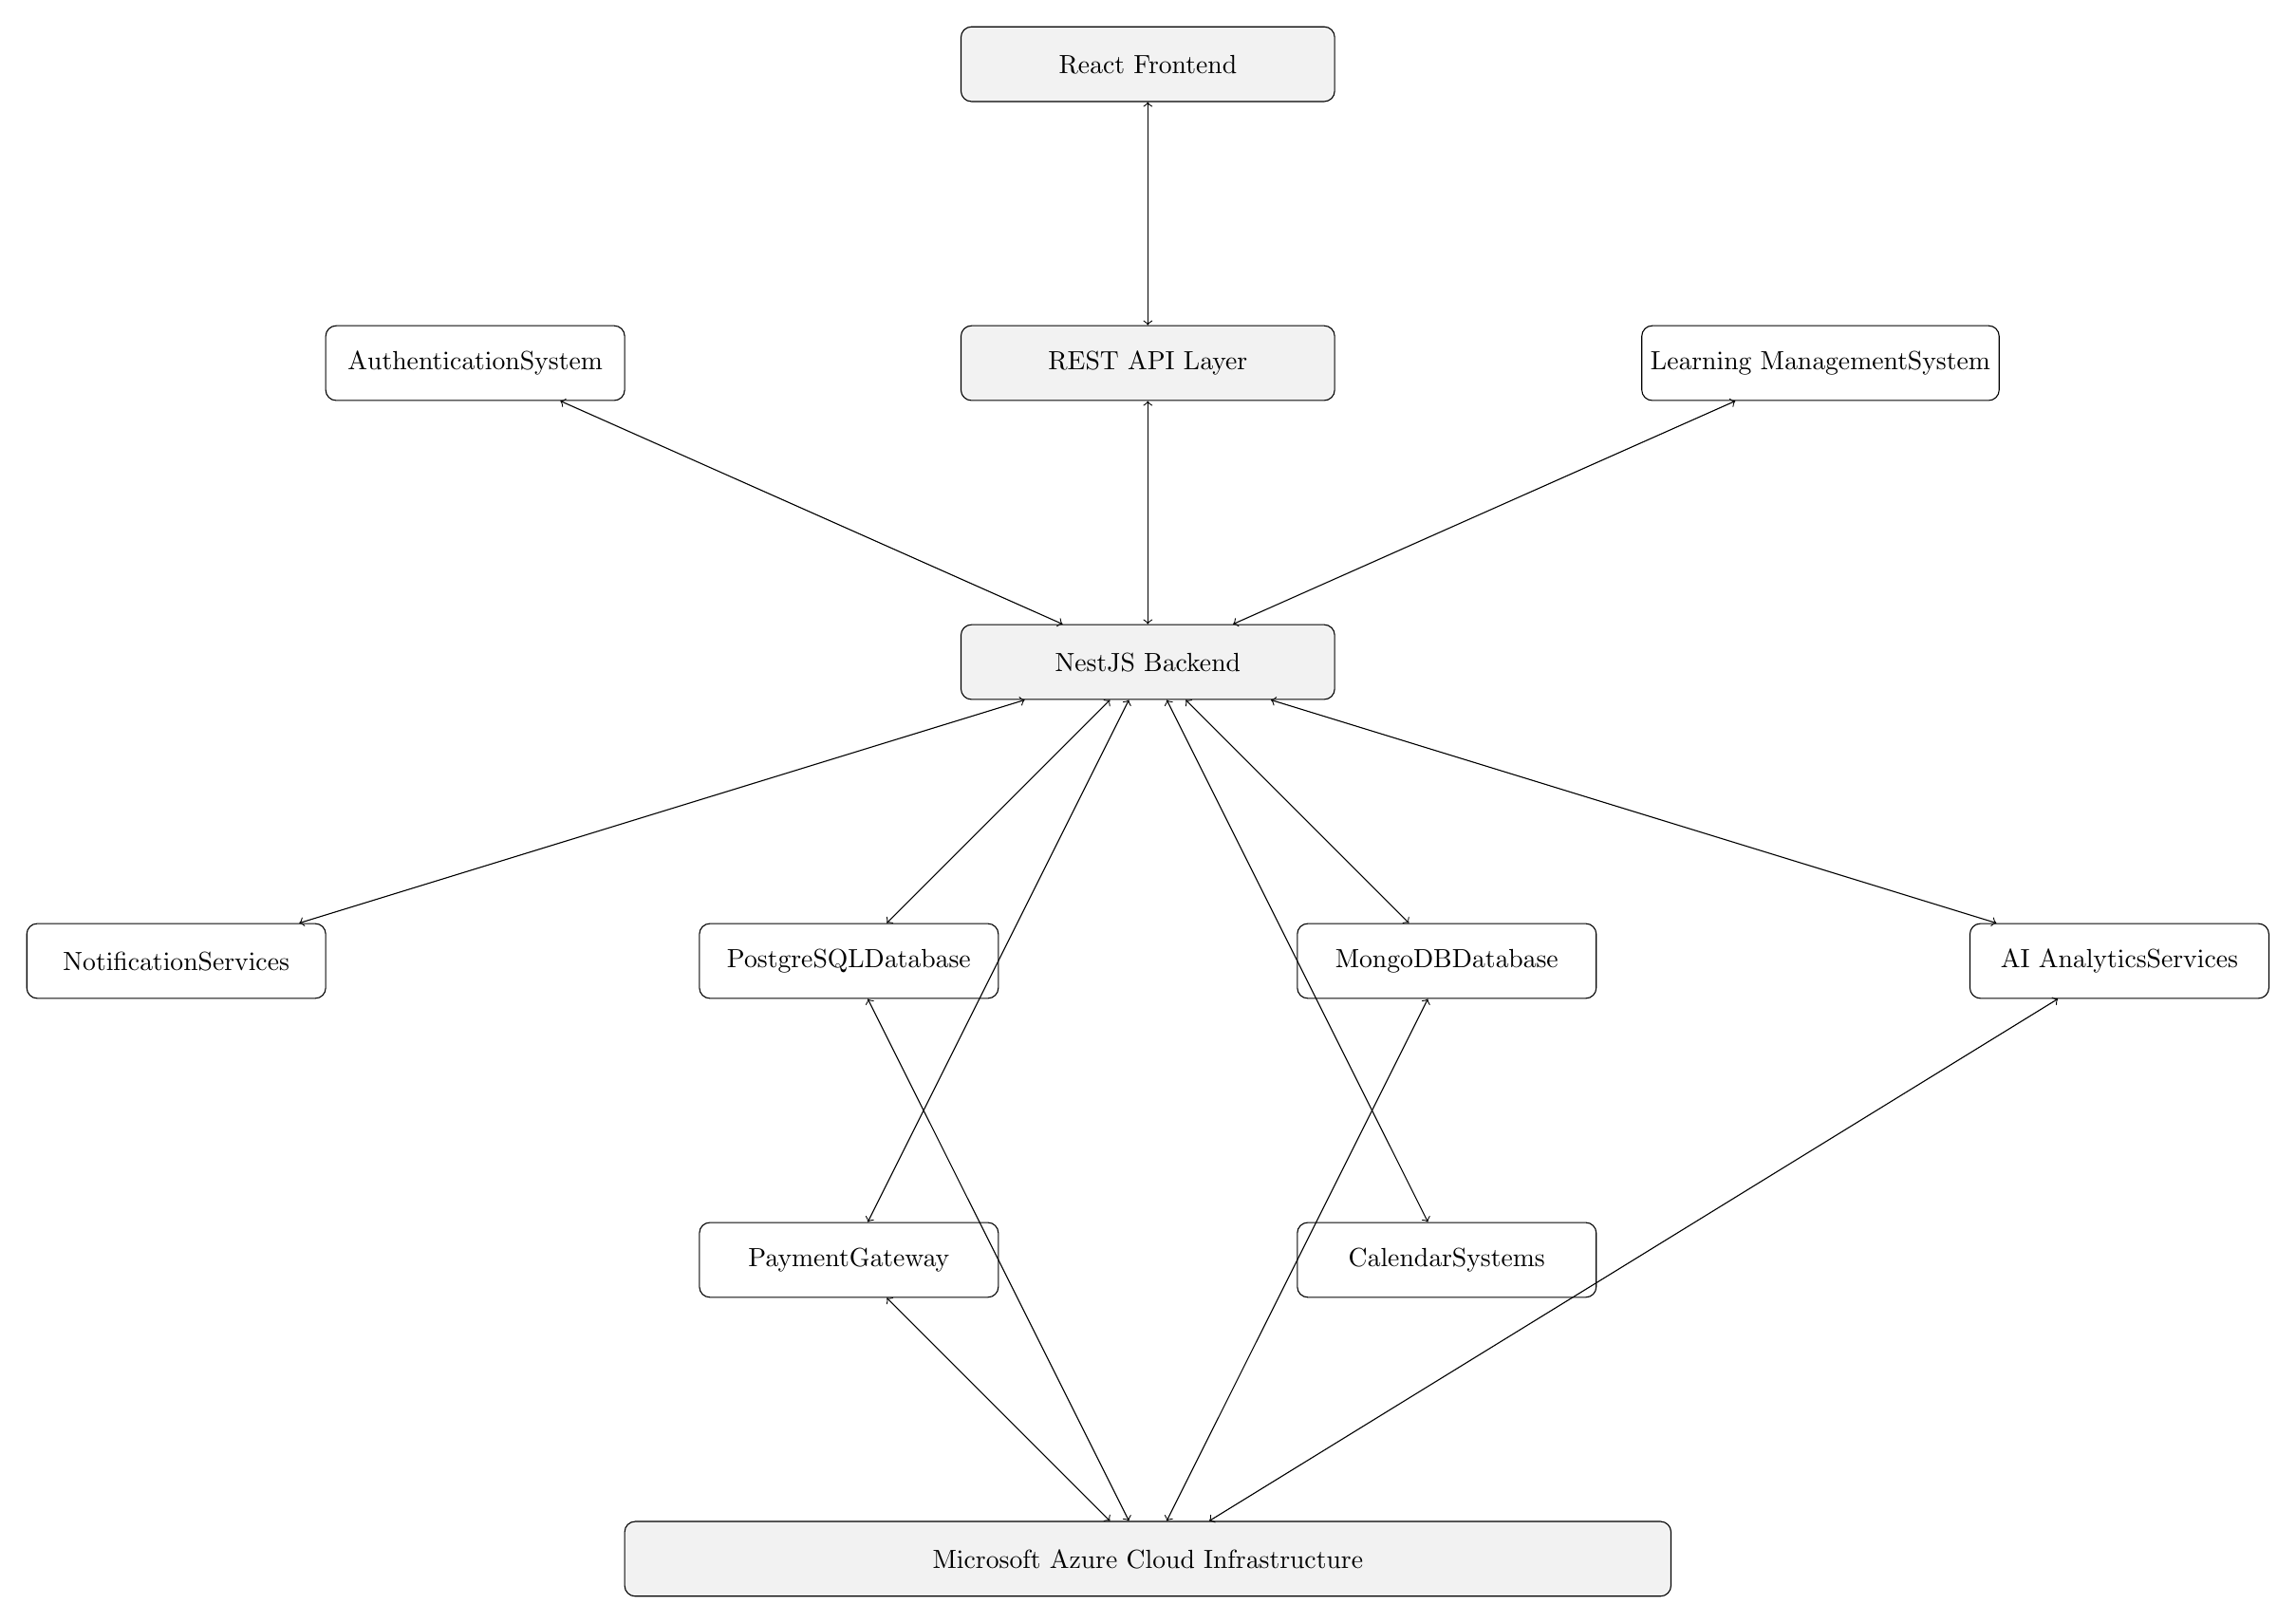
\begin{tikzpicture}[node distance=3cm]
\node (frontend) [rectangle, rounded corners, minimum width=5cm, minimum height=1cm, text centered, draw=black, fill=gray!10] {React Frontend};

\node (api) [rectangle, rounded corners, minimum width=5cm, minimum height=1cm, text centered, draw=black, fill=gray!10, below of=frontend, yshift=-1cm] {REST API Layer};

\node (backend) [rectangle, rounded corners, minimum width=5cm, minimum height=1cm, text centered, draw=black, fill=gray!10, below of=api, yshift=-1cm] {NestJS Backend};

\node (auth) [rectangle, rounded corners, minimum width=4cm, minimum height=1cm, text centered, draw=black, left of=api, xshift=-6cm] {Authentication\\ System};

\node (lms) [rectangle, rounded corners, minimum width=4cm, minimum height=1cm, text centered, draw=black, right of=api, xshift=6cm] {Learning Management\\ System};

\node (postgres) [rectangle, rounded corners, minimum width=4cm, minimum height=1cm, text centered, draw=black, below of=backend, xshift=-4cm, yshift=-1cm] {PostgreSQL\\ Database};

\node (mongodb) [rectangle, rounded corners, minimum width=4cm, minimum height=1cm, text centered, draw=black, below of=backend, xshift=4cm, yshift=-1cm] {MongoDB\\ Database};

\node (notification) [rectangle, rounded corners, minimum width=4cm, minimum height=1cm, text centered, draw=black, left of=postgres, xshift=-6cm] {Notification\\ Services};

\node (ai) [rectangle, rounded corners, minimum width=4cm, minimum height=1cm, text centered, draw=black, right of=mongodb, xshift=6cm] {AI Analytics\\ Services};

\node (payment) [rectangle, rounded corners, minimum width=4cm, minimum height=1cm, text centered, draw=black, below of=postgres, yshift=-1cm] {Payment\\ Gateway};

\node (calendar) [rectangle, rounded corners, minimum width=4cm, minimum height=1cm, text centered, draw=black, below of=mongodb, yshift=-1cm] {Calendar\\ Systems};

\node (cloud) [rectangle, rounded corners, minimum width=14cm, minimum height=1cm, text centered, draw=black, fill=gray!10, below of=payment, xshift=4cm, yshift=-1cm] {Microsoft Azure Cloud Infrastructure};

\draw[<->] (frontend) -- (api);
\draw[<->] (api) -- (backend);
\draw[<->] (backend) -- (postgres);
\draw[<->] (backend) -- (mongodb);
\draw[<->] (backend) -- (auth);
\draw[<->] (backend) -- (lms);
\draw[<->] (backend) -- (notification);
\draw[<->] (backend) -- (ai);
\draw[<->] (backend) -- (payment);
\draw[<->] (backend) -- (calendar);
\draw[<->] (postgres) -- (cloud);
\draw[<->] (mongodb) -- (cloud);
\draw[<->] (payment) -- (cloud);
\draw[<->] (ai) -- (cloud);

\end{tikzpicture}
\caption{System integration flow with external services}
\end{figure}
\end{landscape}

\section{Key Integrations}

\begin{table}[H]
\centering
\begin{tabular}{|p{3.5cm}|p{5cm}|p{6cm}|}
\hline
\textbf{Integration Type} & \textbf{Purpose} & \textbf{Implementation Approach} \\
\hline
Authentication Systems & Single sign-on capabilities & \begin{itemize}
\item Azure Active Directory integration
\item SAML 2.0 and OAuth 2.0 support
\item JWT token exchange mechanisms
\end{itemize} \\
\hline
Learning Management Systems & Synchronize course content and grades & \begin{itemize}
\item LTI (Learning Tools Interoperability) standard
\item REST APIs for data exchange
\item Scheduled synchronization jobs
\end{itemize} \\
\hline
Financial Systems & Fee management and payment processing & \begin{itemize}
\item Payment gateway integrations
\item Financial record synchronization
\item Invoice generation and tracking
\end{itemize} \\
\hline
Notification Services & Multi-channel alerting & \begin{itemize}
\item Email service integration (SMTP/API)
\item SMS gateway connections
\item Push notification services
\end{itemize} \\
\hline
Calendar Systems & Schedule synchronization & \begin{itemize}
\item iCal standard support
\item Google/Microsoft calendar integration
\cm, text centered, draw=black, below of=decision, xshift=-5cm, yshift=-1.2cm] {Message Teacher};

\node (admin) [rectangle, rounded corners, minimum width=4cm, minimum height=0.8cm, text centered, draw=black, below of=decision, xshift=5cm, yshift=-1.2cm] {Contact Administration};

\node (compose) [rectangle, rounded corners, minimum width=4cm, minimum height=0.8cm, text centered, draw=black, below of=teacher, yshift=-0.8cm] {Compose message};

\node (admin_form) [rectangle, rounded corners, minimum width=4cm, minimum height=0.8cm, text centered, draw=black, below of=admin, yshift=-0.8cm] {Fill contact form};

\node (topics) [rectangle, rounded corners, minimum width=5cm, minimum height=1.5cm, text centered, draw=black, below of=compose, yshift=-0.8cm] {- Attendance issues\\ - Academic performance\\ - Assignment clarifications};

\node (admin_topics) [rectangle, rounded corners, minimum width=5cm, minimum height=1.5cm, text centered, draw=black, below of=admin_form, yshift=-0.8cm] {- Administrative requests\\ - Account issues\\ - General feedback};

\node (follow_up) [rectangle, rounded corners, minimum width=6cm, minimum height=0.8cm, text centered, draw=black, below of=topics, xshift=2.5cm, yshift=-2cm] {Parent receives notification when response arrives};

\node (history) [rectangle, rounded corners, minimum width=6cm, minimum height=0.8cm, text centered, draw=black, below of=follow_up, yshift=-0.8cm] {Communication history available for reference};

\draw[->] (login) -- (dashboard);
\draw[->] (dashboard) -- (child);
\draw[->] (child) -- (decision);
\draw[->] (decision) -- (teacher) node[midway, above, sloped] {Teacher};
\draw[->] (decision) -- (admin) node[midway, above, sloped] {Administration};
\draw[->] (teacher) -- (compose);
\draw[->] (admin) -- (admin_form);
\draw[->] (compose) -- (topics);
\draw[->] (admin_form) -- (admin_topics);
\draw[->] (topics) |- (follow_up);
\draw[->] (admin_topics) |- (follow_up);
\draw[->] (follow_up) -- (history);
\end{tikzpicture}
}
\caption{Parent communication workflow}
\end{figure}

\section{Student Workflows}

\subsection{Student Assignment Submission Workflow}

\begin{figure}[H]
\centering
\resizebox{\textwidth}{!}{
\begin{tikzpicture}[node distance=2.5cm]
\node (login) [rectangle, rounded corners, minimum width=4cm, minimum height=0.8cm, text centered, draw=black] {Student logs into system};

\node (dashboard) [rectangle, rounded corners, minimum width=4cm, minimum height=0.8cm, text centered, draw=black, below of=login] {Student views dashboard};

\node (assignments) [rectangle, rounded corners, minimum width=4cm, minimum height=0.8cm, text centered, draw=black, below of=dashboard] {Student opens Assignments section};

\node (view) [rectangle, rounded corners, minimum width=4.5cm, minimum height=0.8cm, text centered, draw=black, below of=assignments] {Student views assignment details};

\node (work) [rectangle, rounded corners, minimum width=4.5cm, minimum height=0.8cm, text centered, draw=black, below of=view] {Student completes assignment offline};

\node (upload) [rectangle, rounded corners, minimum width=4cm, minimum height=0.8cm, text centered, draw=black, below of=work] {Student uploads work to system};

\node (decision) [diamond, minimum width=2.5cm, minimum height=1.5cm, text centered, draw=black, below of=upload, yshift=-1.2cm] {Online?};

\node (submit_online) [rectangle, rounded corners, minimum width=4cm, minimum height=0.8cm, text centered, draw=black, below of=decision, xshift=-4.5cm, yshift=-1.2cm] {Work submitted directly};

\node (store_offline) [rectangle, rounded corners, minimum width=4cm, minimum height=0.8cm, text centered, draw=black, below of=decision, xshift=4.5cm, yshift=-1.2cm] {Work stored locally in browser};

\node (confirm_online) [rectangle, rounded corners, minimum width=4cm, minimum height=0.8cm, text centered, draw=black, below of=submit_online, yshift=-0.8cm] {System confirms submission};

\node (sync) [rectangle, rounded corners, minimum width=4cm, minimum height=0.8cm, text centered, draw=black, below of=store_offline, yshift=-0.8cm] {Auto-sync when online again};

\node (teacher) [rectangle, rounded corners, minimum width=5cm, minimum height=0.8cm, text centered, draw=black, below of=confirm_online, yshift=-1.8cm] {Assignment available for teacher review};

\node (feedback) [rectangle, rounded corners, minimum width=5cm, minimum height=0.8cm, text centered, draw=black, below of=teacher, yshift=-0.8cm] {Student later receives grade and feedback};

\draw[->] (login) -- (dashboard);
\draw[->] (dashboard) -- (assignments);
\draw[->] (assignments) -- (view);
\draw[->] (view) -- (work);
\draw[->] (work) -- (upload);
\draw[->] (upload) -- (decision);
\draw[->] (decision) -- (submit_online) node[midway, above, sloped] {Yes};
\draw[->] (decision) -- (store_offline) node[midway, above, sloped] {No};
\draw[->] (submit_online) -- (confirm_online);
\draw[->] (store_offline) -- (sync);
\draw[->] (confirm_online) -- (teacher);
\draw[->] (sync) |- (teacher);
\draw[->] (teacher) -- (feedback);
\end{tikzpicture}
}
\caption{Student workflow for assignment submission}
\end{figure}

\subsection{Student Schedule and Grades Review Workflow}

\begin{figure}[H]
\centering
\resizebox{\textwidth}{!}{
\begin{tikzpicture}[node distance=2.5cm]
\node (login) [rectangle, rounded corners, minimum width=4cm, minimum height=0.8cm, text centered, draw=black] {Student logs into system};

\node (dashboard) [rectangle, rounded corners, minimum width=4cm, minimum height=0.8cm, text centered, draw=black, below of=login] {Student views dashboard};

\node (decision) [diamond, minimum width=3.2cm, minimum height=1.8cm, text centered, draw=black, below of=dashboard, yshift=-1.2cm] {Information\\ to View?};

\node (schedule) [rectangle, rounded corners, minimum width=3.5cm, minimum height=0.8cm, text centered, draw=black, below of=decision, xshift=-5.5cm, yshift=-1.2cm] {Class Schedule};

\node (grades) [rectangle, rounded corners, minimum width=3.5cm, minimum height=0.8cm, text centered, draw=black, below of=decision, yshift=-1.2cm] {Academic Grades};

\node (tasks) [rectangle, rounded corners, minimum width=3.5cm, minimum height=0.8cm, text centered, draw=black, below of=decision, xshift=5.5cm, yshift=-1.2cm] {Upcoming Tasks};

\node (view_schedule) [rectangle, rounded corners, minimum width=3.5cm, minimum height=0.8cm, text centered, draw=black, below of=schedule, yshift=-0.8cm] {Daily/weekly timetable};

\node (view_grades) [rectangle, rounded corners, minimum width=3.5cm, minimum height=0.8cm, text centered, draw=black, below of=grades, yshift=-0.8cm] {Subject-wise performance};

\node (view_tasks) [rectangle, rounded corners, minimum width=3.5cm, minimum height=0.8cm, text centered, draw=black, below of=tasks, yshift=-0.8cm] {Assignments/test dates};

\node (detail) [rectangle, rounded corners, minimum width=5cm, minimum height=0.8cm, text centered, draw=black, below of=view_grades, yshift=-1.8cm] {Student can drill down for details};

\node (action) [rectangle, rounded corners, minimum width=5.5cm, minimum height=0.8cm, text centered, draw=black, below of=detail, yshift=-0.8cm] {Student can take appropriate actions based on data};

\node (offline) [rectangle, rounded corners, minimum width=5cm, minimum height=0.8cm, text centered, draw=black, below of=action, yshift=-0.8cm] {Information available offline if previously loaded};

\draw[->] (login) -- (dashboard);
\draw[->] (dashboard) -- (decision);
\draw[->] (decision) -- (schedule) node[midway, above, sloped] {Schedule};
\draw[->] (decision) -- (grades) node[midway, above] {Grades};
\draw[->] (decision) -- (tasks) node[midway, above, sloped] {Tasks};
\draw[->] (schedule) -- (view_schedule);
\draw[->] (grades) -- (view_grades);
\draw[->] (tasks) -- (view_tasks);
\draw[->] (view_schedule) |- (detail);
\draw[->] (view_grades) -- (detail);
\draw[->] (view_tasks) |- (detail);
\draw[->] (detail) -- (action);
\draw[->] (action) -- (offline);
\end{tikzpicture}
}
\caption{Student workflow for schedule and grades review}
\end{figure}

\chapter{Key Implementation Challenges \& Mitigation Strategies}

During the implementation of the school management system, several technical and organizational challenges are anticipated. This section outlines these challenges and provides strategies to address them effectively.

\section{Technical Challenges}

\begin{table}[H]
\centering
\begin{tabular}{|p{3.5cm}|p{5.5cm}|p{5.5cm}|}
\hline
\textbf{Challenge} & \textbf{Description} & \textbf{Mitigation Strategy} \\
\hline
Data Migration & Transferring existing student, teacher, and academic records from legacy systems & \begin{itemize}
\item Develop specialized ETL scripts
\item Implement a phased migration approach
\item Provide a transitional period with both systems
\end{itemize} \\
\hline
Offline Reliability & Ensuring data integrity during offline usage and synchronization & \begin{itemize}
\item Robust conflict resolution mechanisms
\item Clear timestamp-based precedence rules
\item Comprehensive sync status indicators
\end{itemize} \\
\hline
Performance at Scale & Maintaining responsive performance with large datasets and concurrent users & \begin{itemize}
\item Implement database indexing strategies
\item Use caching for frequently accessed data
\item Design for horizontal scalability on Azure
\end{itemize} \\
\hline
AI Model Accuracy & Building accurate prediction and facial recognition models & \begin{itemize}
\item Start with conservative, high-confidence predictions
\item Continuously improve models with new data
\item Provide manual override options
\end{itemize} \\
\hline
Security & Protecting sensitive student data and preventing unauthorized access & \begin{itemize}
\item Regular security audits and penetration testing
\item End-to-end encryption for sensitive data
\item Comprehensive role-based access controls
\end{itemize} \\
\hline
\end{tabular}
\caption{Technical implementation challenges and mitigation strategies}
\end{table}

\section{Organizational Challenges}

\begin{table}[H]
\centering
\begin{tabular}{|p{3.5cm}|p{5.5cm}|p{5.5cm}|}
\hline
\textbf{Challenge} & \textbf{Description} & \textbf{Mitigation Strategy} \\
\hline
User Adoption & Ensuring stakeholders embrace and effectively use the new system & \begin{itemize}
\item Comprehensive training program
\item Intuitive UX design for minimal learning curve
\item Designated "super users" within each user group
\end{itemize} \\
\hline
Changing Requirements & Managing evolving requirements during implementation & \begin{itemize}
\item Agile methodology for adaptability
\item Regular stakeholder feedback sessions
\item Modular design for feature flexibility
\end{itemize} \\
\hline
Training & Educating staff, parents, and students on system usage & \begin{itemize}
\item Role-specific training materials and videos
\item In-app guided tours and contextual help
\item Support desk during initial deployment
\end{itemize} \\
\hline
Workflow Integration & Adapting the system to existing school processes & \begin{itemize}
\item Process mapping workshops before implementation
\item Configurable workflows in the system
\item Phased approach to process changes
\end{itemize} \\
\hline
Stakeholder Alignment & Managing expectations across diverse stakeholder groups & \begin{itemize}
\item Regular progress updates and demos
\item Clear communication about features and limitations
\item Feedback channels for continuous improvement
\end{itemize} \\
\hline
\end{tabular}
\caption{Organizational implementation challenges and mitigation strategies}
\end{table}

\chapter{Data Security \& Compliance}

Protecting sensitive student and academic data is a critical aspect of the school management system implementation. This section outlines the comprehensive security measures and compliance considerations incorporated into the design.

\section{Security Architecture}

\begin{figure}[H]
\centering
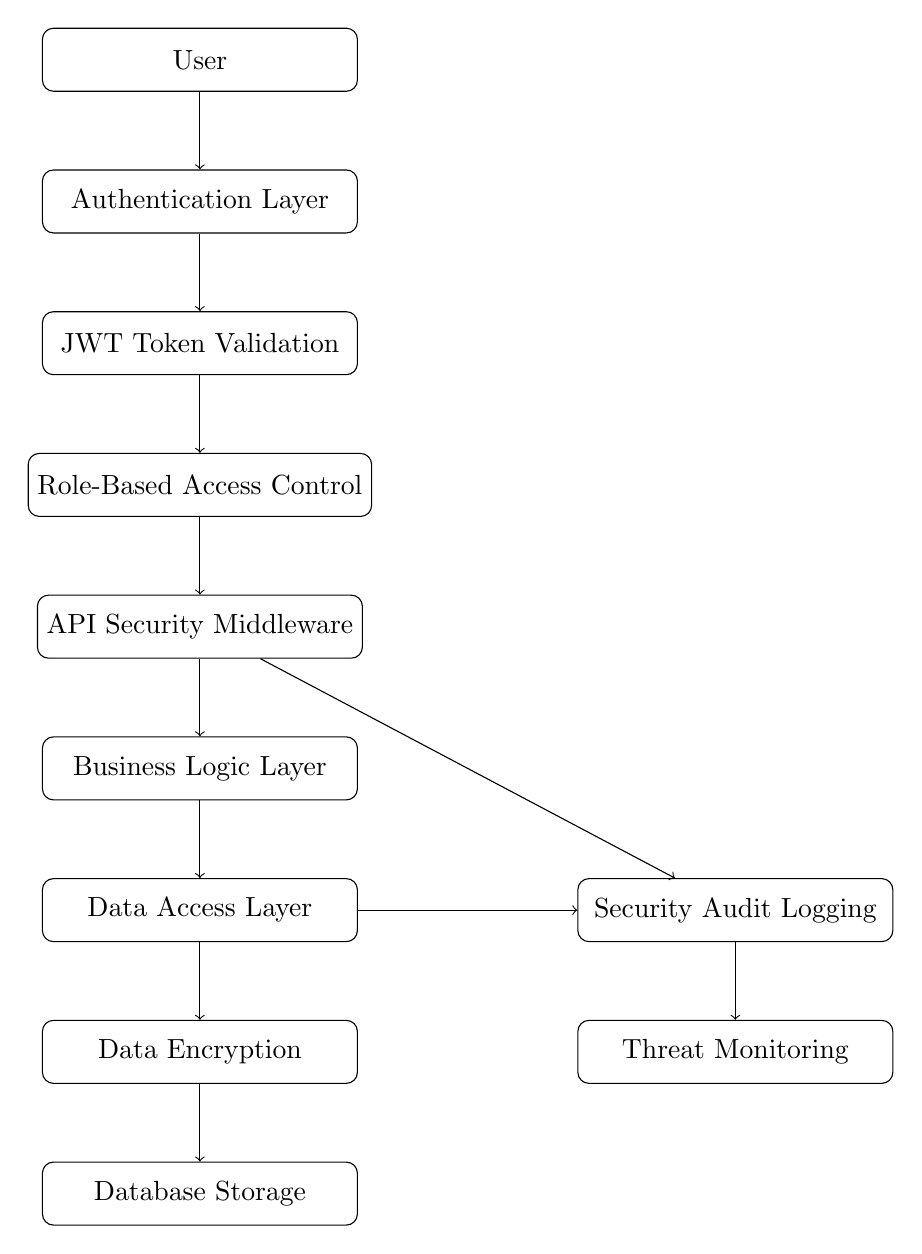
\begin{tikzpicture}[node distance=1.8cm]
\node (user) [rectangle, rounded corners, minimum width=4cm, minimum height=0.8cm, text centered, draw=black] {User};

\node (auth) [rectangle, rounded corners, minimum width=4cm, minimum height=0.8cm, text centered, draw=black, below of=user] {Authentication Layer};

\node (jwt) [rectangle, rounded corners, minimum width=4cm, minimum height=0.8cm, text centered, draw=black, below of=auth] {JWT Token Validation};

\node (rbac) [rectangle, rounded corners, minimum width=4cm, minimum height=0.8cm, text centered, draw=black, below of=jwt] {Role-Based Access Control};

\node (api) [rectangle, rounded corners, minimum width=4cm, minimum height=0.8cm, text centered, draw=black, below of=rbac] {API Security Middleware};

\node (business) [rectangle, rounded corners, minimum width=4cm, minimum height=0.8cm, text centered, draw=black, below of=api] {Business Logic Layer};

\node (data) [rectangle, rounded corners, minimum width=4cm, minimum height=0.8cm, text centered, draw=black, below of=business] {Data Access Layer};

\node (encryption) [rectangle, rounded corners, minimum width=4cm, minimum height=0.8cm, text centered, draw=black, below of=data] {Data Encryption};

\node (database) [rectangle, rounded corners, minimum width=4cm, minimum height=0.8cm, text centered, draw=black, below of=encryption] {Database Storage};

\node (logging) [rectangle, rounded corners, minimum width=4cm, minimum height=0.8cm, text centered, draw=black, right of=data, xshift=5cm] {Security Audit Logging};

\node (monitoring) [rectangle, rounded corners, minimum width=4cm, minimum height=0.8cm, text centered, draw=black, below of=logging] {Threat Monitoring};

\draw[->] (user) -- (auth);
\draw[->] (auth) -- (jwt);
\draw[->] (jwt) -- (rbac);
\draw[->] (rbac) -- (api);
\draw[->] (api) -- (business);
\draw[->] (business) -- (data);
\draw[->] (data) -- (encryption);
\draw[->] (encryption) -- (database);
\draw[->] (api) -- (logging);
\draw[->] (data) -- (logging);
\draw[->] (logging) -- (monitoring);

\end{tikzpicture}
\caption{Security architecture of the school management system}
\end{figure}

\section{Security Measures}

\begin{itemize}
    \item \textbf{Authentication:} Multi-factor authentication for administrative accounts, strong password policies, and secure password reset mechanisms.
    
    \item \textbf{Authorization:} Granular role-based access control ensuring users only access data appropriate to their role.
    
    \item \textbf{Data Encryption:} All sensitive data encrypted both in transit (HTTPS/TLS) and at rest (AES-256 encryption).
    
    \item \textbf{Secure APIs:} API endpoints protected against common vulnerabilities (injection, XSS, CSRF) with input validation and sanitization.
    
    \item \textbf{Audit Logging:} Comprehensive logging of all security-relevant events and access to sensitive data.
    
    \item \textbf{Regular Security Testing:} Scheduled penetration testing and vulnerability assessments.
    
    \item \textbf{Secure Development:} Following secure coding practices and regular dependency vulnerability scanning.
    
    \item \textbf{Data Minimization:} Collecting and storing only necessary data to reduce exposure risk.
\end{itemize}

\section{Compliance Considerations}

\begin{table}[H]
\centering
\begin{tabular}{|p{3cm}|p{11.5cm}|}
\hline
\textbf{Regulation} & \textbf{Implementation Approach} \\
\hline
FERPA (USA) & \begin{itemize}
\item Parental consent for sharing student information
\item Audit trails for all data access
\item Strict access controls limiting data visibility
\item Ability to generate compliance reports
\end{itemize} \\
\hline
GDPR (EU) & \begin{itemize}
\item Data processing consent management
\item Right to access, rectification, and erasure mechanisms
\item Data breach notification capabilities
\item Data retention policies and automated purging
\end{itemize} \\
\hline
COPPA (USA) & \begin{itemize}
\item Age verification for student accounts
\item Parental consent management
\item Limited data collection from minors
\item Simplified privacy notices
\end{itemize} \\
\hline
Local Education Laws & \begin{itemize}
\item Configurable data retention policies
\item Compliance reporting capabilities
\item Adaptable privacy controls for regional requirements
\end{itemize} \\
\hline
\end{tabular}
\caption{Compliance considerations and implementation approaches}
\end{table}    /guards             # Role-based guards
  /users                # User management module
  /classes              # Class management module
  /attendance           # Attendance module
  /grades               # Grading module
  /notifications        # Notification module
  /reports              # Reporting module
  /analytics            # Analytics and AI module
  /common               # Shared utilities and interfaces
\end{verbatim}

\section{Database Schemas}

\subsection{PostgreSQL Entity Relationships}
Key entity relationships include:
\begin{itemize}
    \item Users with role-based differentiation
    \item One-to-many relationship between Teachers and Classes
    \item Many-to-many relationship between Students and Classes (via Enrollments)
    \item One-to-many relationship between Classes and Assignments
    \item One-to-many relationship between Students and Grades
\end{itemize}

\subsection{MongoDB Collections}
\begin{itemize}
    \item \textbf{Logs:} System events, user actions, errors
    \item \textbf{Analytics:} Computed insights and aggregated data
    \item \textbf{OfflineSync:} Temporary storage for offline actions
    \item \textbf{AIInsights:} Machine learning results and predictions
\end{itemize}

\section{API Design}

\subsection{RESTful Endpoints}
The API follows RESTful principles with these key endpoints:

\begin{itemize}
    \item \textbf{Authentication:} \texttt{/api/v1/auth/login}, \texttt{/api/v1/auth/refresh}
    \item \textbf{User Management:} \texttt{/api/v1/users}, \texttt{/api/v1/users/:id}
    \item \textbf{Classes:} \texttt{/api/v1/classes}, \texttt{/api/v1/classes/:id}
    \item \textbf{Students:} \texttt{/api/v1/students}, \texttt{/api/v1/classes/:id/students}
    \item \textbf{Attendance:} \texttt{/api/v1/attendance}, \texttt{/api/v1/attendance/batch}
    \item \textbf{Grades:} \texttt{/api/v1/grades}, \texttt{/api/v1/students/:id/grades}
    \item \textbf{Notifications:} \texttt{/api/v1/notifications}, \texttt{/api/v1/users/:id/notifications}
    \item \textbf{Reports:} \texttt{/api/v1/reports/attendance}, \texttt{/api/v1/reports/performance}
    \item \textbf{AI Services:} \texttt{/api/v1/ai/face-recognition}, \texttt{/api/v1/ai/analytics}
\end{itemize}

\subsection{Authentication Flow}
\begin{enumerate}
    \item User submits credentials
    \item Server validates and issues JWT token with appropriate role claims
    \item Client stores token securely and includes in Authorization header
    \item Protected endpoints verify token and roles before processing
    \item Refresh tokens handle session extension without re-login
\end{enumerate}

\section{Azure Cloud Architecture}

\subsection{Containerization Strategy}
\begin{itemize}
    \item Application components packaged as Docker containers
    \item Container images stored in Azure Container Registry
    \item Orchestration through Azure Kubernetes Service
    \item Horizontal scaling based on demand metrics
\end{itemize}

\subsection{Azure Resources}
\begin{figure}[H]
\centering
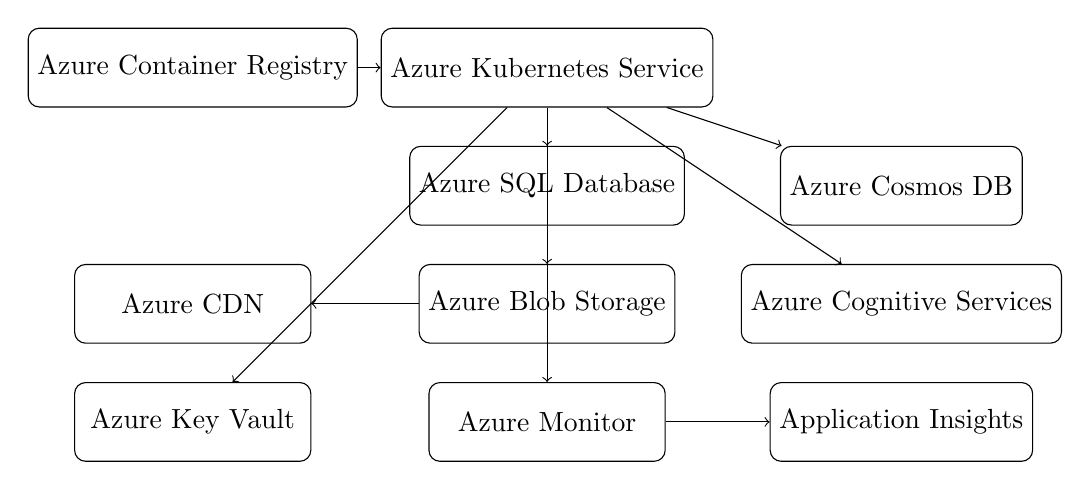
\begin{tikzpicture}[node distance=1.5cm]
\node (aks) [rectangle, rounded corners, minimum width=3cm, minimum height=1cm, text centered, draw=black] {Azure Kubernetes Service};
\node (acr) [rectangle, rounded corners, minimum width=3cm, minimum height=1cm, text centered, draw=black, left of=aks, xshift=-3cm] {Azure Container Registry};
\node (sql) [rectangle, rounded corners, minimum width=3cm, minimum height=1cm, text centered, draw=black, below of=aks] {Azure SQL Database};
\node (cosmos) [rectangle, rounded corners, minimum width=3cm, minimum height=1cm, text centered, draw=black, right of=sql, xshift=3cm] {Azure Cosmos DB};
\node (storage) [rectangle, rounded corners, minimum width=3cm, minimum height=1cm, text centered, draw=black, below of=sql] {Azure Blob Storage};
\node (cdn) [rectangle, rounded corners, minimum width=3cm, minimum height=1cm, text centered, draw=black, left of=storage, xshift=-3cm] {Azure CDN};
\node (cog) [rectangle, rounded corners, minimum width=3cm, minimum height=1cm, text centered, draw=black, right of=storage, xshift=3cm] {Azure Cognitive Services};
\node (monitor) [rectangle, rounded corners, minimum width=3cm, minimum height=1cm, text centered, draw=black, below of=storage] {Azure Monitor};
\node (keyvault) [rectangle, rounded corners, minimum width=3cm, minimum height=1cm, text centered, draw=black, left of=monitor, xshift=-3cm] {Azure Key Vault};
\node (appinsights) [rectangle, rounded corners, minimum width=3cm, minimum height=1cm, text centered, draw=black, right of=monitor, xshift=3cm] {Application Insights};

\draw[->] (acr) -- (aks);
\draw[->] (aks) -- (sql);
\draw[->] (aks) -- (cosmos);
\draw[->] (aks) -- (storage);
\draw[->] (storage) -- (cdn);
\draw[->] (aks) -- (cog);
\draw[->] (aks) -- (monitor);
\draw[->] (aks) -- (keyvault);
\draw[->] (monitor) -- (appinsights);
\end{tikzpicture}
\caption{Azure resources for school management system deployment}
\end{figure}

\subsection{Deployment Pipeline}
\begin{itemize}
    \item Source code managed in GitHub repository
    \item Automated testing with GitHub Actions
    \item Continuous integration building Docker images
    \item Continuous deployment to Azure environments
    \item Separate environments for development, staging, and production
    \item Infrastructure as Code using Azure Resource Manager templates
\end{itemize}

\chapter{User Workflows}

This chapter details the typical user interaction flows for each type of user in the system.

\section{Teacher Workflows}

\subsection{Attendance Tracking Workflow}

\begin{figure}[H]
\centering
\resizebox{\textwidth}{!}{
\begin{tikzpicture}[node distance=2.5cm]
\node (login) [rectangle, rounded corners, minimum width=4cm, minimum height=0.8cm, text centered, draw=black] {Teacher logs into the system};

\node (dashboard) [rectangle, rounded corners, minimum width=4cm, minimum height=0.8cm, text centered, draw=black, below of=login] {Teacher accesses dashboard};

\node (class) [rectangle, rounded corners, minimum width=4cm, minimum height=0.8cm, text centered, draw=black, below of=dashboard] {Teacher selects class to manage};

\node (attendance) [rectangle, rounded corners, minimum width=4cm, minimum height=0.8cm, text centered, draw=black, below of=class] {Teacher opens attendance module};

\node (decision) [diamond, minimum width=2.5cm, minimum height=1.5cm, text centered, draw=black, below of=attendance, yshift=-1.2cm] {Online?};

\node (mark_online) [rectangle, rounded corners, minimum width=4cm, minimum height=0.8cm, text centered, draw=black, below of=decision, xshift=-4.5cm, yshift=-1.2cm] {Mark attendance directly in system};

\node (mark_offline) [rectangle, rounded corners, minimum width=4cm, minimum height=0.8cm, text centered, draw=black, below of=decision, xshift=4.5cm, yshift=-1.2cm] {Mark attendance in offline mode};

\node (save_online) [rectangle, rounded corners, minimum width=4cm, minimum height=0.8cm, text centered, draw=black, below of=mark_online, yshift=-0.5cm] {Data saved to database immediately};

\node (save_offline) [rectangle, rounded corners, minimum width=4cm, minimum height=0.8cm, text centered, draw=black, below of=mark_offline, yshift=-0.5cm] {Data stored in IndexedDB};

\node (sync) [rectangle, rounded corners, minimum width=4cm, minimum height=0.8cm, text centered, draw=black, below of=save_offline, yshift=-0.5cm] {Auto-sync when back online};

\node (notify) [rectangle, rounded corners, minimum width=6cm, minimum height=0.8cm, text centered, draw=black, below of=save_online, xshift=4.5cm, yshift=-1.8cm] {System sends notifications to parents of absent students};

\node (report) [rectangle, rounded corners, minimum width=6cm, minimum height=0.8cm, text centered, draw=black, below of=notify, yshift=-0.8cm] {Attendance data available for reporting and analytics};

\draw[->] (login) -- (dashboard);
\draw[->] (dashboard) -- (class);
\draw[->] (class) -- (attendance);
\draw[->] (attendance) -- (decision);
\draw[->] (decision) -- (mark_online) node[midway, above, sloped] {Yes};
\draw[->] (decision) -- (mark_offline) node[midway, above, sloped] {No};
\draw[->] (mark_online) -- (save_online);
\draw[->] (mark_offline) -- (save_offline);
\draw[->] (save_offline) -- (sync);
\draw[->] (save_online) -- (notify);
\draw[->] (sync) -- (notify);
\draw[->] (notify) -- (report);
\end{tikzpicture}
}
\caption{Teacher workflow for attendance tracking}
\end{figure}

\subsection{Grade Entry Workflow}

\begin{figure}[H]
\centering
\resizebox{\textwidth}{!}{
\begin{tikzpicture}[node distance=2.5cm]
\node (login) [rectangle, rounded corners, minimum width=4cm, minimum height=0.8cm, text centered, draw=black] {Teacher logs into the system};

\node (dashboard) [rectangle, rounded corners, minimum width=4cm, minimum height=0.8cm, text centered, draw=black, below of=login] {Teacher accesses dashboard};

\node (class) [rectangle, rounded corners, minimum width=4cm, minimum height=0.8cm, text centered, draw=black, below of=dashboard] {Teacher selects class to manage};

\node (grades) [rectangle, rounded corners, minimum width=4cm, minimum height=0.8cm, text centered, draw=black, below of=class] {Teacher opens grading module};

\node (create) [rectangle, rounded corners, minimum width=4.5cm, minimum height=0.8cm, text centered, draw=black, below of=grades] {Teacher creates new assignment/test};

\node (enter) [rectangle, rounded corners, minimum width=4cm, minimum height=0.8cm, text centered, draw=black, below of=create] {Teacher enters grades for students};

\node (decision) [diamond, minimum width=2.5cm, minimum height=1.5cm, text centered, draw=black, below of=enter, yshift=-1.2cm] {Online?};

\node (save_online) [rectangle, rounded corners, minimum width=4cm, minimum height=0.8cm, text centered, draw=black, below of=decision, xshift=-4.5cm, yshift=-1.2cm] {Grades saved directly to database};

\node (save_offline) [rectangle, rounded corners, minimum width=4cm, minimum height=0.8cm, text centered, draw=black, below of=decision, xshift=4.5cm, yshift=-1.2cm] {Grades stored locally in IndexedDB};

\node (sync) [rectangle, rounded corners, minimum width=4cm, minimum height=0.8cm, text centered, draw=black, below of=save_offline, yshift=-0.5cm] {Auto-sync when connectivity returns};

\node (analyze) [rectangle, rounded corners, minimum width=4cm, minimum height=0.8cm, text centered, draw=black, below of=save_online, yshift=-1.8cm] {System analyzes grade patterns};

\node (notify) [rectangle, rounded corners, minimum width=4.5cm, minimum height=0.8cm, text centered, draw=black, below of=analyze, yshift=-0.8cm] {Parents/students notified of new grades};

\node (report) [rectangle, rounded corners, minimum width=4cm, minimum height=0.8cm, text centered, draw=black, below of=notify, yshift=-0.8cm] {Grades visible in performance reports};

\draw[->] (login) -- (dashboard);
\draw[->] (dashboard) -- (class);
\draw[->] (class) -- (grades);
\draw[->] (grades) -- (create);
\draw[->] (create) -- (enter);
\draw[->] (enter) -- (decision);
\draw[->] (decision) -- (save_online) node[midway, above, sloped] {Yes};
\draw[->] (decision) -- (save_offline) node[midway, above, sloped] {No};
\draw[->] (save_offline) -- (sync);
\draw[->] (sync) |- (analyze);
\draw[->] (save_online) -- (analyze);
\draw[->] (analyze) -- (notify);
\draw[->] (notify) -- (report);
\end{tikzpicture}
}
\caption{Teacher workflow for grade entry and management}
\end{figure}

\section{Administrator Workflows}

\subsection{Student Registration Workflow}

\begin{figure}[H]
\centering
\resizebox{\textwidth}{!}{
\begin{tikzpicture}[node distance=2.5cm]
\node (login) [rectangle, rounded corners, minimum width=4cm, minimum height=0.8cm, text centered, draw=black] {Admin logs into the system};

\node (dashboard) [rectangle, rounded corners, minimum width=4cm, minimum height=0.8cm, text centered, draw=black, below of=login] {Admin accesses dashboard};

\node (student) [rectangle, rounded corners, minimum width=4cm, minimum height=0.8cm, text centered, draw=black, below of=dashboard] {Admin selects Student Management};

\node (decision) [diamond, minimum width=3cm, minimum height=1.8cm, text centered, draw=black, below of=student, yshift=-1.2cm] {Single or \\ Bulk?};

\node (single) [rectangle, rounded corners, minimum width=4cm, minimum height=0.8cm, text centered, draw=black, below of=decision, xshift=-5cm, yshift=-1.2cm] {Admin fills student form manually};

\node (bulk) [rectangle, rounded corners, minimum width=4cm, minimum height=0.8cm, text centered, draw=black, below of=decision, xshift=5cm, yshift=-1.2cm] {Admin uploads CSV/Excel file};

\node (manual_save) [rectangle, rounded corners, minimum width=4cm, minimum height=0.8cm, text centered, draw=black, below of=single, yshift=-0.8cm] {System validates and saves record};

\node (process) [rectangle, rounded corners, minimum width=4cm, minimum height=0.8cm, text centered, draw=black, below of=bulk, yshift=-0.8cm] {System processes file rows};

\node (validation) [rectangle, rounded corners, minimum width=4cm, minimum height=0.8cm, text centered, draw=black, below of=process, yshift=-0.8cm] {System validates all entries};

\node (report_single) [rectangle, rounded corners, minimum width=4cm, minimum height=0.8cm, text centered, draw=black, below of=manual_save, yshift=-0.8cm] {Confirmation shown to admin};

\node (import) [rectangle, rounded corners, minimum width=4cm, minimum height=0.8cm, text centered, draw=black, below of=validation, yshift=-0.8cm] {Valid records imported to database};

\node (report_bulk) [rectangle, rounded corners, minimum width=5cm, minimum height=0.8cm, text centered, draw=black, below of=import, yshift=-0.8cm] {Import summary report displayed};

\node (account) [rectangle, rounded corners, minimum width=6cm, minimum height=0.8cm, text centered, draw=black, below of=report_single, xshift=4.5cm, yshift=-2cm] {Student accounts marked as pending activation};

\node (notify) [rectangle, rounded corners, minimum width=6cm, minimum height=0.8cm, text centered, draw=black, below of=account, yshift=-0.8cm] {Optional: Welcome emails sent to parents/students};

\draw[->] (login) -- (dashboard);
\draw[->] (dashboard) -- (student);
\draw[->] (student) -- (decision);
\draw[->] (decision) -- (single) node[midway, above, sloped] {Single};
\draw[->] (decision) -- (bulk) node[midway, above, sloped] {Bulk};
\draw[->] (single) -- (manual_save);
\draw[->] (bulk) -- (process);
\draw[->] (process) -- (validation);
\draw[->] (validation) -- (import);
\draw[->] (import) -- (report_bulk);
\draw[->] (manual_save) -- (report_single);
\draw[->] (report_single) |- (account);
\draw[->] (report_bulk) |- (account);
\draw[->] (account) -- (notify);
\end{tikzpicture}
}
\caption{Administrator workflow for student registration}
\end{figure}

\subsection{Report Generation Workflow}

\begin{figure}[H]
\centering
\resizebox{\textwidth}{!}{
\begin{tikzpicture}[node distance=2.5cm]
\node (login) [rectangle, rounded corners, minimum width=4cm, minimum height=0.8cm, text centered, draw=black] {Admin logs into the system};

\node (dashboard) [rectangle, rounded corners, minimum width=4cm, minimum height=0.8cm, text centered, draw=black, below of=login] {Admin accesses dashboard};

\node (reports) [rectangle, rounded corners, minimum width=4cm, minimum height=0.8cm, text centered, draw=black, below of=dashboard] {Admin opens Reports module};

\node (select) [rectangle, rounded corners, minimum width=4cm, minimum height=0.8cm, text centered, draw=black, below of=reports] {Admin selects report type};

\node (params) [rectangle, rounded corners, minimum width=4.5cm, minimum height=0.8cm, text centered, draw=black, below of=select] {Admin configures report parameters};

\node (generate) [rectangle, rounded corners, minimum width=4cm, minimum height=0.8cm, text centered, draw=black, below of=params] {Admin generates report};

\node (process) [rectangle, rounded corners, minimum width=4.5cm, minimum height=0.8cm, text centered, draw=black, below of=generate] {System processes data and analytics};

\node (decision) [diamond, minimum width=3.2cm, minimum height=1.8cm, text centered, draw=black, below of=process, yshift=-1.2cm] {Output Format?};

\node (view) [rectangle, rounded corners, minimum width=4cm, minimum height=0.8cm, text centered, draw=black, below of=decision, xshift=-5cm, yshift=-1.2cm] {View in browser dashboard};

\node (export) [rectangle, rounded corners, minimum width=4cm, minimum height=0.8cm, text centered, draw=black, below of=decision, xshift=5cm, yshift=-1.2cm] {Export as PDF/Excel};

\node (interact) [rectangle, rounded corners, minimum width=4cm, minimum height=0.8cm, text centered, draw=black, below of=view, yshift=-0.8cm] {Interactive visualization};

\node (download) [rectangle, rounded corners, minimum width=4cm, minimum height=0.8cm, text centered, draw=black, below of=export, yshift=-0.8cm] {File download};

\node (share) [rectangle, rounded corners, minimum width=5cm, minimum height=0.8cm, text centered, draw=black, below of=interact, xshift=2.5cm, yshift=-2cm] {Option to share with stakeholders};

\draw[->] (login) -- (dashboard);
\draw[->] (dashboard) -- (reports);
\draw[->] (reports) -- (select);
\draw[->] (select) -- (params);
\draw[->] (params) -- (generate);
\draw[->] (generate) -- (process);
\draw[->] (process) -- (decision);
\draw[->] (decision) -- (view) node[midway, above, sloped] {Browser};
\draw[->] (decision) -- (export) node[midway, above, sloped] {File};
\draw[->] (view) -- (interact);
\draw[->] (export) -- (download);
\draw[->] (interact) -- (share);
\draw[->] (download) -- (share);
\end{tikzpicture}
}
\caption{Administrator workflow for report generation}
\end{figure}

\section{Parent Workflows}

\subsection{Parent Registration and Child Linking Workflow}

\begin{landscape}
\begin{figure}
\centering
\begin{tikzpicture}[node distance=3cm]
\node (start) [rectangle, rounded corners, minimum width=4cm, minimum height=0.8cm, text centered, draw=black] {Parent visits school portal};

\node (register) [rectangle, rounded corners, minimum width=4cm, minimum height=0.8cm, text centered, draw=black, right of=start] {Parent creates new account};

\node (credentials) [rectangle, rounded corners, minimum width=4.5cm, minimum height=0.8cm, text centered, draw=black, right of=register] {Parent enters personal information};

\node (verify) [rectangle, rounded corners, minimum width=4.5cm, minimum height=0.8cm, text centered, draw=black, below of=credentials] {Email verification sent to parent};

\node (confirm) [rectangle, rounded corners, minimum width=4cm, minimum height=0.8cm, text centered, draw=black, below of=verify] {Parent confirms email};

\node (login) [rectangle, rounded corners, minimum width=4cm, minimum height=0.8cm, text centered, draw=black, below of=confirm] {Parent logs into account};

\node (link) [rectangle, rounded corners, minimum width=4.5cm, minimum height=0.8cm, text centered, draw=black, below of=login] {Parent navigates to "Link Child" page};

\node (info) [rectangle, rounded corners, minimum width=5.5cm, minimum height=0.8cm, text centered, draw=black, below of=link] {Parent enters student ID and verification info};

\node (student_check) [diamond, minimum width=2.8cm, minimum height=1.8cm, text centered, draw=black, below of=info, yshift=-1cm] {Valid Student?};

\node (error) [rectangle, rounded corners, minimum width=4cm, minimum height=0.8cm, text centered, draw=black, left of=student_check, xshift=-3cm] {Error message displayed};

\node (system_link) [rectangle, rounded corners, minimum width=4.5cm, minimum height=0.8cm, text centered, draw=black, below of=student_check, yshift=-1.2cm] {System links parent to student};

\node (approval) [diamond, minimum width=3.2cm, minimum height=2cm, text centered, draw=black, below of=system_link, yshift=-1.2cm] {Admin Approval\\ Required?};

\node (pending) [rectangle, rounded corners, minimum width=4.5cm, minimum height=0.8cm, text centered, draw=black, left of=approval, xshift=-3cm] {Link pending admin approval};

\node (admin_review) [rectangle, rounded corners, minimum width=4cm, minimum height=0.8cm, text centered, draw=black, below of=pending] {Admin reviews request};

\node (approval_decision) [diamond, minimum width=2.8cm, minimum height=1.8cm, text centered, draw=black, below of=admin_review, yshift=-1cm] {Approved?};

\node (decline) [rectangle, rounded corners, minimum width=4cm, minimum height=0.8cm, text centered, draw=black, left of=approval_decision, xshift=-3cm] {Link rejected};

\node (immediate) [rectangle, rounded corners, minimum width=4.5cm, minimum height=0.8cm, text centered, draw=black, right of=approval, xshift=3cm] {Link approved immediately};

\node (access) [rectangle, rounded corners, minimum width=5cm, minimum height=0.8cm, text centered, draw=black, below of=immediate, yshift=-3cm] {Parent granted access to child's data};

\node (dashboard) [rectangle, rounded corners, minimum width=5cm, minimum height=0.8cm, text centered, draw=black, below of=access] {Parent views child's dashboard};

\draw[->] (start) -- (register);
\draw[->] (register) -- (credentials);
\draw[->] (credentials) -- (verify);
\draw[->] (verify) -- (confirm);
\draw[->] (confirm) -- (login);
\draw[->] (login) -- (link);
\draw[->] (link) -- (info);
\draw[->] (info) -- (student_check);
\draw[->] (student_check) -- (error) node[midway, above] {No};
\draw[->] (error) |- (info);
\draw[->] (student_check) -- (system_link) node[midway, right] {Yes};
\draw[->] (system_link) -- (approval);
\draw[->] (approval) -- (immediate) node[midway, above] {No};
\draw[->] (approval) -- (pending) node[midway, above] {Yes};
\draw[->] (pending) -- (admin_review);
\draw[->] (admin_review) -- (approval_decision);
\draw[->] (approval_decision) -- (decline) node[midway, above] {No};
\draw[->] (approval_decision) |- (access) node[pos=0.25, above] {Yes};
\draw[->] (immediate) -- (access);
\draw[->] (access) -- (dashboard);

\end{tikzpicture}
\caption{Parent registration and child linking workflow}
\end{figure}
\end{landscape}

\subsection{Parent Monitoring Child's Progress Workflow}

\begin{figure}[H]
\centering
\resizebox{\textwidth}{!}{
\begin{tikzpicture}[node distance=2.5cm]
\node (login) [rectangle, rounded corners, minimum width=4cm, minimum height=0.8cm, text centered, draw=black] {Parent logs into system};

\node (dashboard) [rectangle, rounded corners, minimum width=4cm, minimum height=0.8cm, text centered, draw=black, below of=login] {Parent views dashboard};

\node (select) [rectangle, rounded corners, minimum width=4cm, minimum height=0.8cm, text centered, draw=black, below of=dashboard] {Parent selects child (if multiple)};

\node (overview) [rectangle, rounded corners, minimum width=4.5cm, minimum height=0.8cm, text centered, draw=black, below of=select] {Parent views child's overview};

\node (decision) [diamond, minimum width=3.2cm, minimum height=1.8cm, text centered, draw=black, below of=overview, yshift=-1.2cm] {Area to\\ Review?};

\node (grades) [rectangle, rounded corners, minimum width=3.5cm, minimum height=0.8cm, text centered, draw=black, below of=decision, xshift=-5.5cm, yshift=-1.2cm] {Academic Performance};

\node (attendance) [rectangle, rounded corners, minimum width=3.5cm, minimum height=0.8cm, text centered, draw=black, below of=decision, yshift=-1.2cm] {Attendance History};

\node (behavior) [rectangle, rounded corners, minimum width=3.5cm, minimum height=0.8cm, text centered, draw=black, below of=decision, xshift=5.5cm, yshift=-1.2cm] {Upcoming Tasks};

\node (grade_detail) [rectangle, rounded corners, minimum width=3.5cm, minimum height=0.8cm, text centered, draw=black, below of=grades, yshift=-0.8cm] {Review grades and feedback};

\node (attend_detail) [rectangle, rounded corners, minimum width=3.5cm, minimum height=0.8cm, text centered, draw=black, below of=attendance, yshift=-0.8cm] {View attendance patterns};

\node (task_detail) [rectangle, rounded corners, minimum width=3.5cm, minimum height=0.8cm, text centered, draw=black, below of=behavior, yshift=-0.8cm] {Check assignments/exams};

\node (contact) [rectangle, rounded corners, minimum width=5cm, minimum height=0.8cm, text centered, draw=black, below of=attend_detail, yshift=-2cm] {Option to contact teacher directly};

\node (download) [rectangle, rounded corners, minimum width=5cm, minimum height=0.8cm, text centered, draw=black, below of=contact, yshift=-0.8cm] {Download/print reports if needed};

\draw[->] (login) -- (dashboard);
\draw[->] (dashboard) -- (select);
\draw[->] (select) -- (overview);
\draw[->] (overview) -- (decision);
\draw[->] (decision) -- (grades) node[midway, above, sloped] {Grades};
\draw[->] (decision) -- (attendance) node[midway, above] {Attendance};
\draw[->] (decision) -- (behavior) node[midway, above, sloped] {Tasks};
\draw[->] (grades) -- (grade_detail);
\draw[->] (attendance) -- (attend_detail);
\draw[->] (behavior) -- (task_detail);
\draw[->] (grade_detail) |- (contact);
\draw[->] (attend_detail) -- (contact);
\draw[->] (task_detail) |- (contact);
\draw[->] (contact) -- (download);
\end{tikzpicture}
}
\caption{Parent workflow for monitoring child's progress}
\end{figure}

\subsection{Parent Communication Workflow}


\begin{figure}[H]
\centering
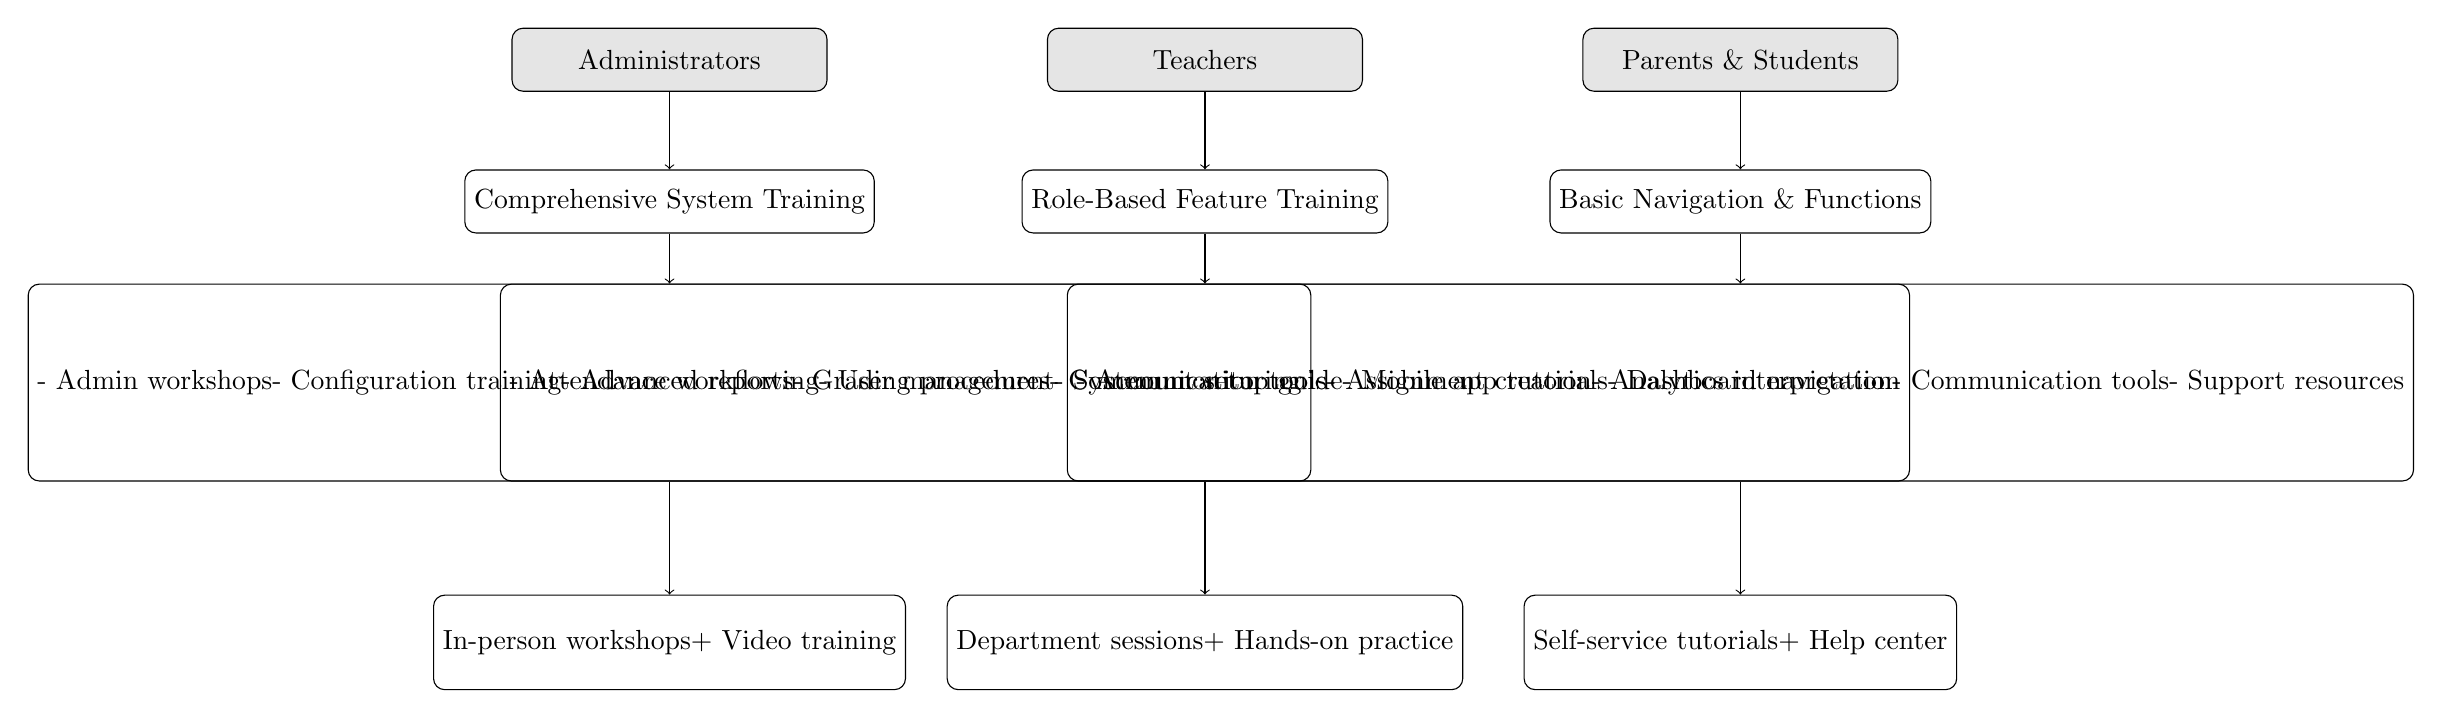
\begin{tikzpicture}[node distance=1.8cm]
\node (admin) [rectangle, rounded corners, minimum width=4cm, minimum height=0.8cm, text centered, draw=black, fill=gray!20] {Administrators};
\node (teacher) [rectangle, rounded corners, minimum width=4cm, minimum height=0.8cm, text centered, draw=black, fill=gray!20, right of=admin, xshift=5cm] {Teachers};
\node (parent) [rectangle, rounded corners, minimum width=4cm, minimum height=0.8cm, text centered, draw=black, fill=gray!20, right of=teacher, xshift=5cm] {Parents \& Students};

\node (training1) [rectangle, rounded corners, minimum width=4cm, minimum height=0.8cm, text centered, draw=black, below of=admin] {Comprehensive System Training};
\node (training2) [rectangle, rounded corners, minimum width=4cm, minimum height=0.8cm, text centered, draw=black, below of=teacher] {Role-Based Feature Training};
\node (training3) [rectangle, rounded corners, minimum width=4cm, minimum height=0.8cm, text centered, draw=black, below of=parent] {Basic Navigation \& Functions};

\node (material1) [rectangle, rounded corners, minimum width=4cm, minimum height=2.5cm, text centered, draw=black, below of=training1, yshift=-0.5cm] {- Admin workshops\\ - Configuration training\\ - Advanced reporting\\ - User management\\ - System monitoring};
\node (material2) [rectangle, rounded corners, minimum width=4cm, minimum height=2.5cm, text centered, draw=black, below of=training2, yshift=-0.5cm] {- Attendance workflows\\ - Grading procedures\\ - Communication tools\\ - Assignment creation\\ - Analytics interpretation};
\node (material3) [rectangle, rounded corners, minimum width=4cm, minimum height=2.5cm, text centered, draw=black, below of=training3, yshift=-0.5cm] {- Account setup guide\\ - Mobile app tutorials\\ - Dashboard navigation\\ - Communication tools\\ - Support resources};

\node (delivery1) [rectangle, rounded corners, minimum width=4cm, minimum height=1.2cm, text centered, draw=black, below of=material1, yshift=-1.5cm] {In-person workshops\\ + Video training};
\node (delivery2) [rectangle, rounded corners, minimum width=4cm, minimum height=1.2cm, text centered, draw=black, below of=material2, yshift=-1.5cm] {Department sessions\\ + Hands-on practice};
\node (delivery3) [rectangle, rounded corners, minimum width=4cm, minimum height=1.2cm, text centered, draw=black, below of=material3, yshift=-1.5cm] {Self-service tutorials\\ + Help center};

\draw[->] (admin) -- (training1);
\draw[->] (teacher) -- (training2);
\draw[->] (parent) -- (training3);
\draw[->] (training1) -- (material1);
\draw[->] (training2) -- (material2);
\draw[->] (training3) -- (material3);
\draw[->] (material1) -- (delivery1);
\draw[->] (material2) -- (delivery2);
\draw[->] (material3) -- (delivery3);

\end{tikzpicture}
\caption{Role-based training approach}
\end{figure}

\section{Training Materials}

\begin{itemize}
    \item \textbf{Documentation:} Comprehensive user manuals, quick reference guides, and FAQ documents.
    
    \item \textbf{Video Tutorials:} Role-specific video tutorials demonstrating key system functions.
    
    \item \textbf{Interactive Guides:} In-app walkthroughs and tooltips for key features.
    
    \item \textbf{Training Environments:} Sandbox environments for practice without affecting production data.
    
    \item \textbf{Webinars:} Live and recorded training sessions for different user roles.
    
    \item \textbf{Knowledge Base:} Searchable library of how-to articles and troubleshooting guides.
\end{itemize}

\section{Adoption Strategy}

\begin{figure}[H]
\centering
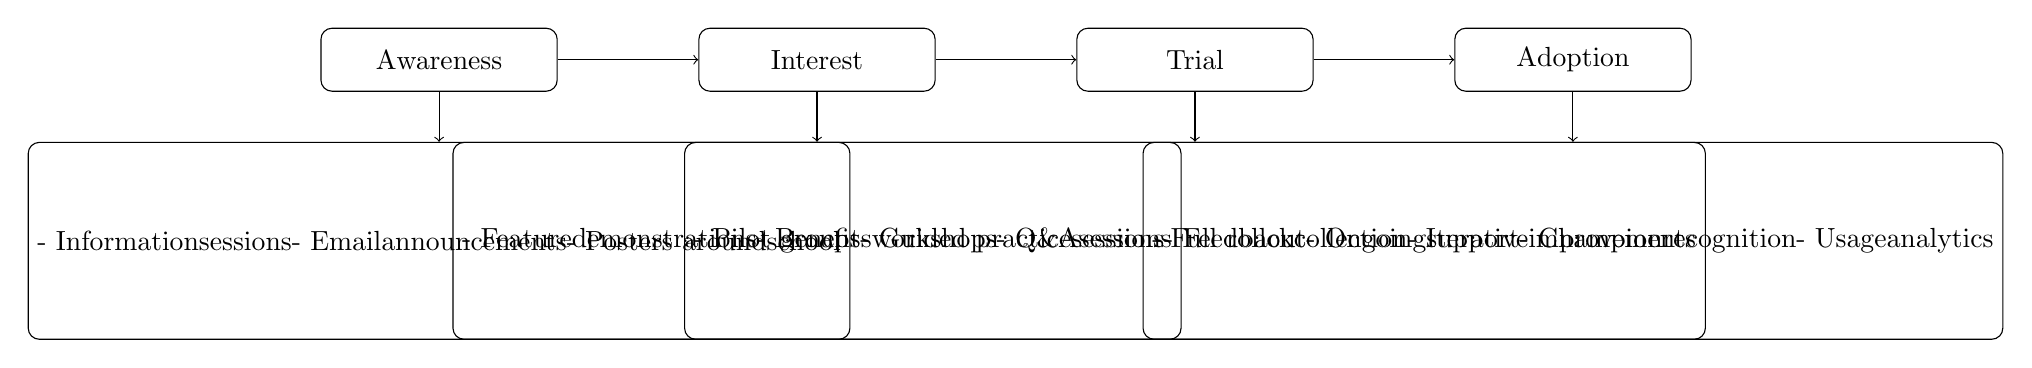
\begin{tikzpicture}[node distance=1.8cm]

\node (awareness) [rectangle, rounded corners, minimum width=3cm, minimum height=0.8cm, text centered, draw=black] {Awareness};
\node (interest) [rectangle, rounded corners, minimum width=3cm, minimum height=0.8cm, text centered, draw=black, right of=awareness, xshift=3cm] {Interest};
\node (trial) [rectangle, rounded corners, minimum width=3cm, minimum height=0.8cm, text centered, draw=black, right of=interest, xshift=3cm] {Trial};
\node (adoption) [rectangle, rounded corners, minimum width=3cm, minimum height=0.8cm, text centered, draw=black, right of=trial, xshift=3cm] {Adoption};

\node (activity1) [rectangle, rounded corners, minimum width=3cm, minimum height=2.5cm, text centered, draw=black, below of=awareness, yshift=-0.5cm] {- Information\\ sessions\\ - Email\\ announcements\\ - Posters around\\ school};
\node (activity2) [rectangle, rounded corners, minimum width=3cm, minimum height=2.5cm, text centered, draw=black, below of=interest, yshift=-0.5cm] {- Feature\\ demonstrations\\ - Benefits\\ workshops\\ - Q\&A\\ sessions};
\node (activity3) [rectangle, rounded corners, minimum width=3cm, minimum height=2.5cm, text centered, draw=black, below of=trial, yshift=-0.5cm] {- Pilot groups\\ - Guided practice\\ sessions\\ - Feedback\\ collection\\ - Iterative\\ improvements};
\node (activity4) [rectangle, rounded corners, minimum width=3cm, minimum height=2.5cm, text centered, draw=black, below of=adoption, yshift=-0.5cm] {- Full rollout\\ - Ongoing\\ support\\ - Champion\\ recognition\\ - Usage\\ analytics};

\draw[->] (awareness) -- (interest);
\draw[->] (interest) -- (trial);
\draw[->] (trial) -- (adoption);
\draw[->] (awareness) -- (activity1);
\draw[->] (interest) -- (activity2);
\draw[->] (trial) -- (activity3);
\draw[->] (adoption) -- (activity4);

\end{tikzpicture}
\caption{Phased adoption strategy}
\end{figure}

\section{Support Infrastructure}

\begin{itemize}
    \item \textbf{Help Desk:} Dedicated support team available during implementation and early adoption phases.
    
    \item \textbf{Super Users:} Identified power users within each stakeholder group who receive advanced training and act as first-line support.
    
    \item \textbf{Feedback Mechanisms:} In-app feedback tools and regular surveys to identify usability issues or training gaps.
    
    \item \textbf{Support Tiers:} Structured escalation process from basic troubleshooting to advanced technical support.
    
    \item \textbf{Usage Analytics:} Monitoring of system usage patterns to identify features requiring additional training.
\end{itemize}

\chapter{System Integrations}

The school management system is designed to integrate with existing school technology infrastructure and third-party educational systems to create a comprehensive ecosystem.

\section{Integration Architecture}

\begin{landscape}
\begin{figure}
\centering
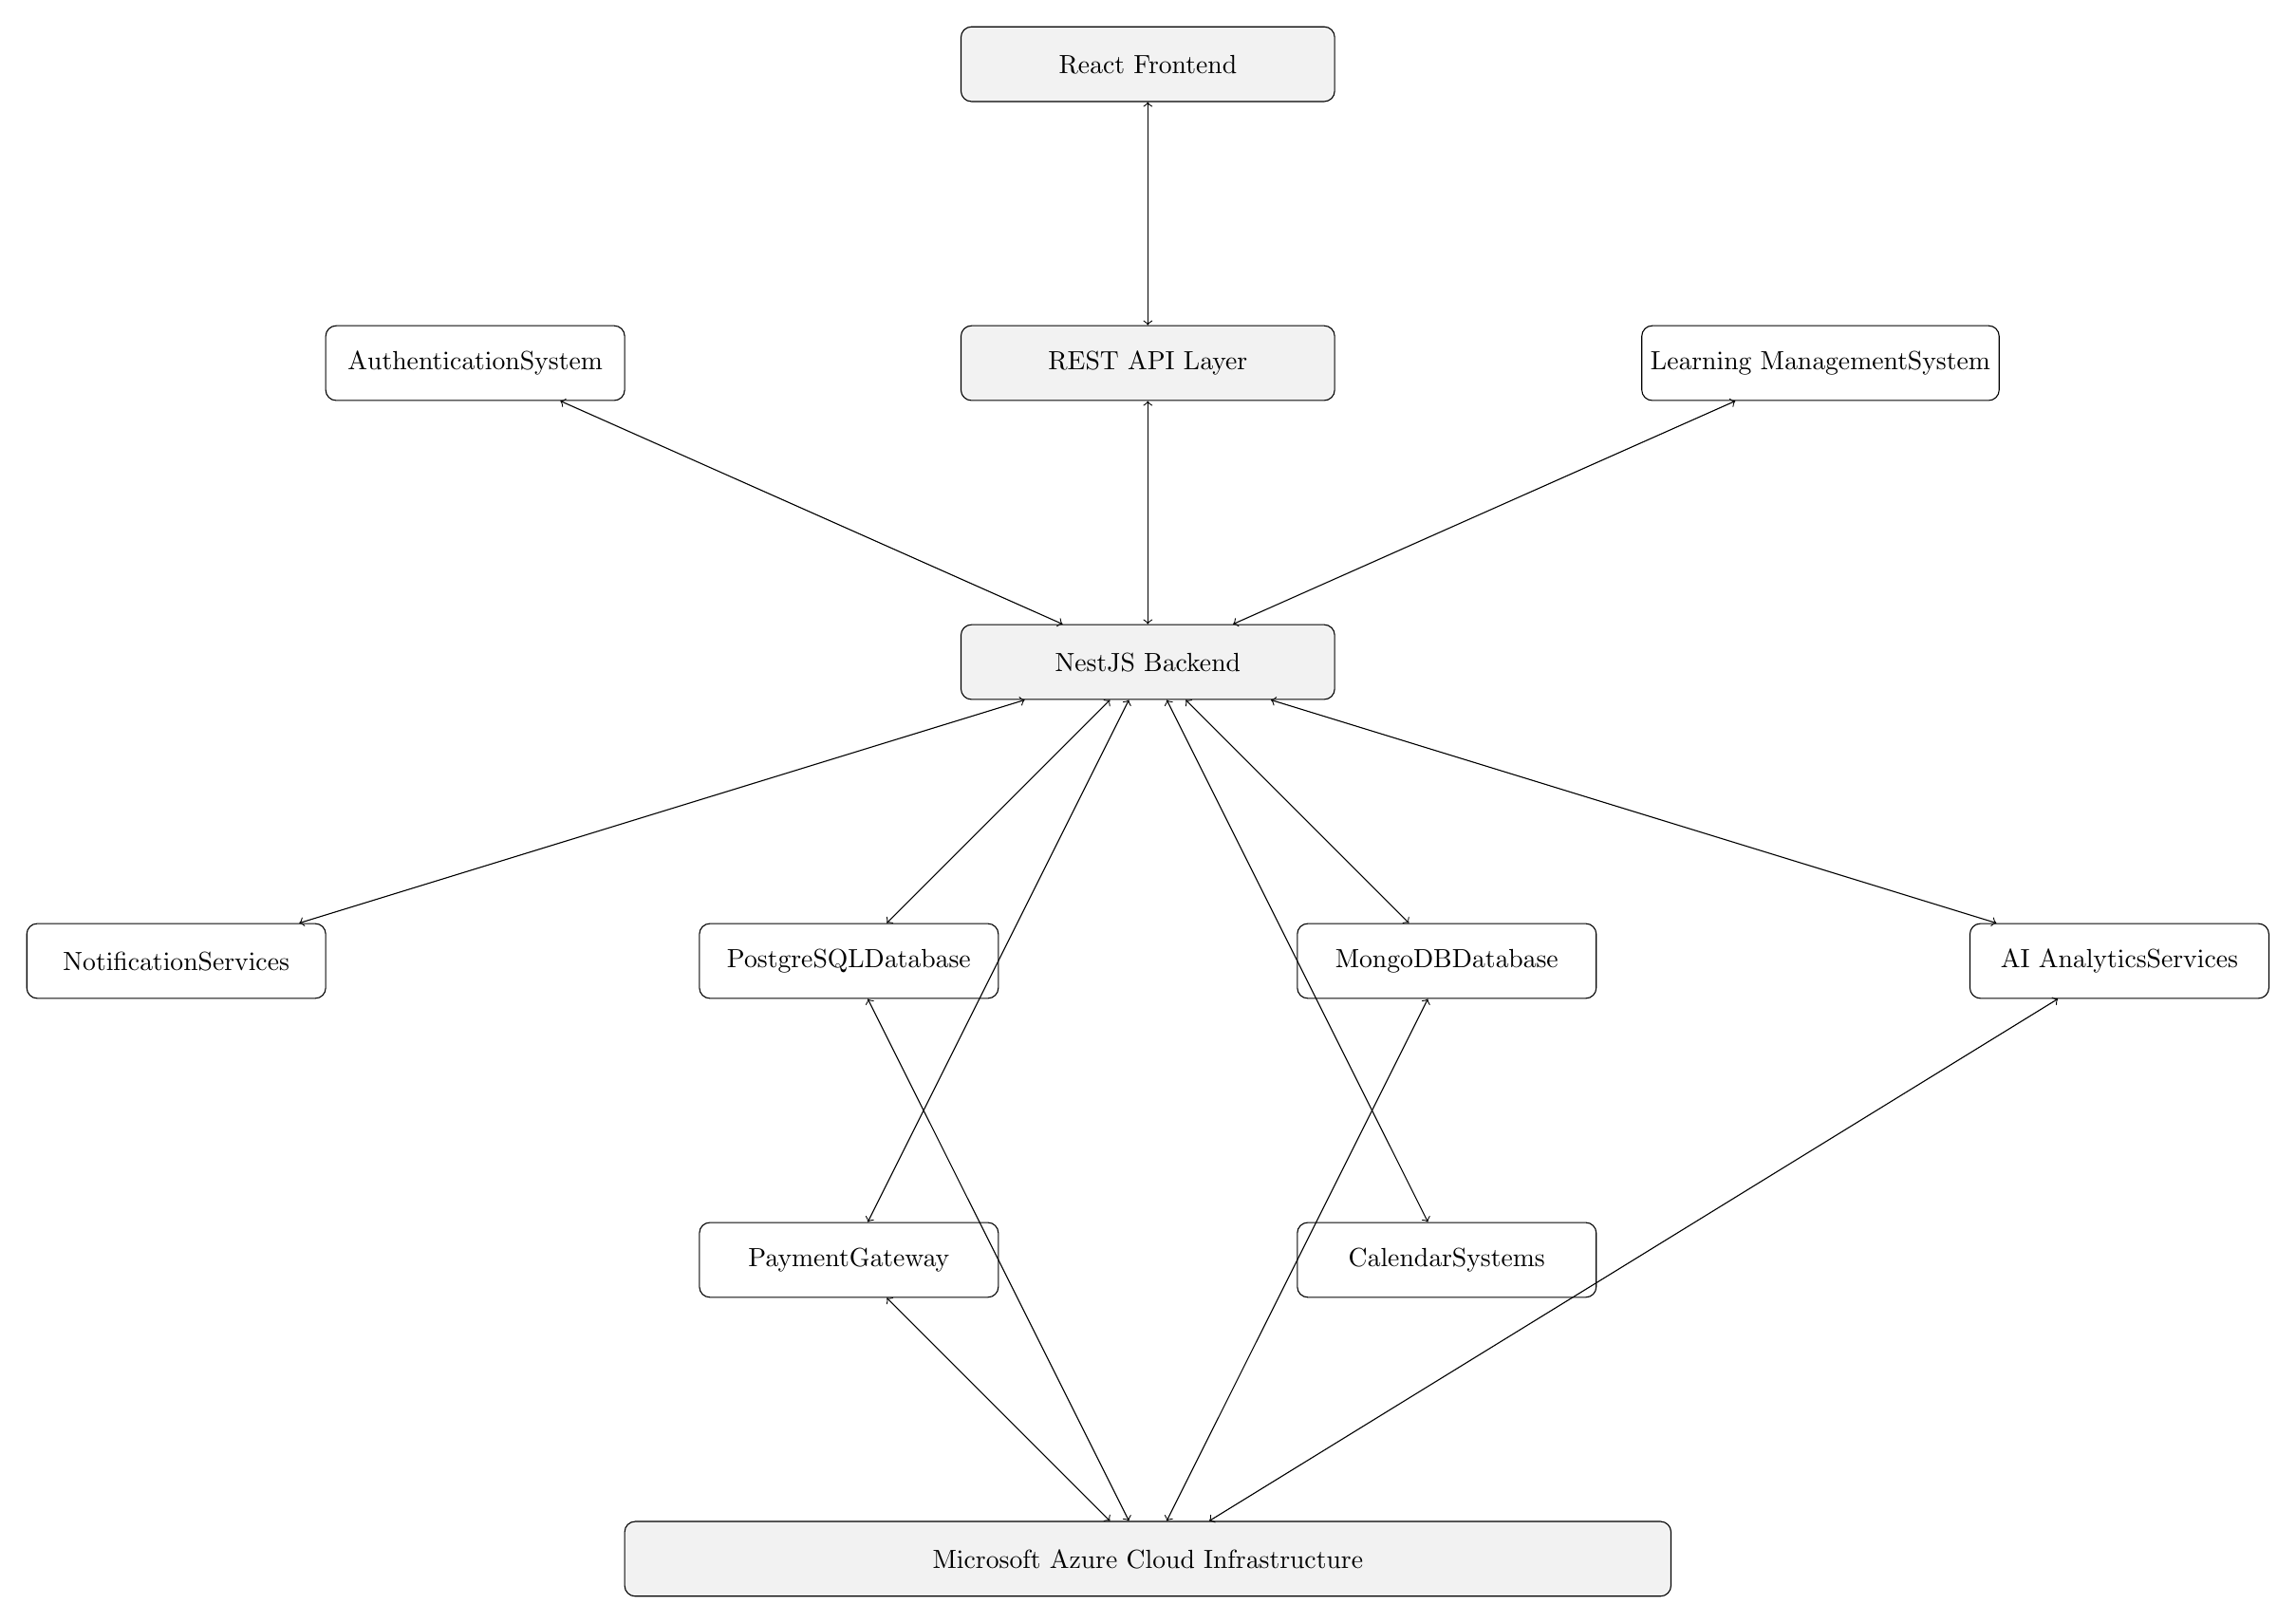
\begin{tikzpicture}[node distance=3cm]
\node (frontend) [rectangle, rounded corners, minimum width=5cm, minimum height=1cm, text centered, draw=black, fill=gray!10] {React Frontend};

\node (api) [rectangle, rounded corners, minimum width=5cm, minimum height=1cm, text centered, draw=black, fill=gray!10, below of=frontend, yshift=-1cm] {REST API Layer};

\node (backend) [rectangle, rounded corners, minimum width=5cm, minimum height=1cm, text centered, draw=black, fill=gray!10, below of=api, yshift=-1cm] {NestJS Backend};

\node (auth) [rectangle, rounded corners, minimum width=4cm, minimum height=1cm, text centered, draw=black, left of=api, xshift=-6cm] {Authentication\\ System};

\node (lms) [rectangle, rounded corners, minimum width=4cm, minimum height=1cm, text centered, draw=black, right of=api, xshift=6cm] {Learning Management\\ System};

\node (postgres) [rectangle, rounded corners, minimum width=4cm, minimum height=1cm, text centered, draw=black, below of=backend, xshift=-4cm, yshift=-1cm] {PostgreSQL\\ Database};

\node (mongodb) [rectangle, rounded corners, minimum width=4cm, minimum height=1cm, text centered, draw=black, below of=backend, xshift=4cm, yshift=-1cm] {MongoDB\\ Database};

\node (notification) [rectangle, rounded corners, minimum width=4cm, minimum height=1cm, text centered, draw=black, left of=postgres, xshift=-6cm] {Notification\\ Services};

\node (ai) [rectangle, rounded corners, minimum width=4cm, minimum height=1cm, text centered, draw=black, right of=mongodb, xshift=6cm] {AI Analytics\\ Services};

\node (payment) [rectangle, rounded corners, minimum width=4cm, minimum height=1cm, text centered, draw=black, below of=postgres, yshift=-1cm] {Payment\\ Gateway};

\node (calendar) [rectangle, rounded corners, minimum width=4cm, minimum height=1cm, text centered, draw=black, below of=mongodb, yshift=-1cm] {Calendar\\ Systems};

\node (cloud) [rectangle, rounded corners, minimum width=14cm, minimum height=1cm, text centered, draw=black, fill=gray!10, below of=payment, xshift=4cm, yshift=-1cm] {Microsoft Azure Cloud Infrastructure};

\draw[<->] (frontend) -- (api);
\draw[<->] (api) -- (backend);
\draw[<->] (backend) -- (postgres);
\draw[<->] (backend) -- (mongodb);
\draw[<->] (backend) -- (auth);
\draw[<->] (backend) -- (lms);
\draw[<->] (backend) -- (notification);
\draw[<->] (backend) -- (ai);
\draw[<->] (backend) -- (payment);
\draw[<->] (backend) -- (calendar);
\draw[<->] (postgres) -- (cloud);
\draw[<->] (mongodb) -- (cloud);
\draw[<->] (payment) -- (cloud);
\draw[<->] (ai) -- (cloud);

\end{tikzpicture}
\caption{System integration flow with external services}
\end{figure}
\end{landscape}

\section{Key Integrations}

\begin{table}[H]
\centering
\begin{tabular}{|p{3.5cm}|p{5cm}|p{6cm}|}
\hline
\textbf{Integration Type} & \textbf{Purpose} & \textbf{Implementation Approach} \\
\hline
Authentication Systems & Single sign-on capabilities & \begin{itemize}
\item Azure Active Directory integration
\item SAML 2.0 and OAuth 2.0 support
\item JWT token exchange mechanisms
\end{itemize} \\
\hline
Learning Management Systems & Synchronize course content and grades & \begin{itemize}
\item LTI (Learning Tools Interoperability) standard
\item REST APIs for data exchange
\item Scheduled synchronization jobs
\end{itemize} \\
\hline
Financial Systems & Fee management and payment processing & \begin{itemize}
\item Payment gateway integrations
\item Financial record synchronization
\item Invoice generation and tracking
\end{itemize} \\
\hline
Notification Services & Multi-channel alerting & \begin{itemize}
\item Email service integration (SMTP/API)
\item SMS gateway connections
\item Push notification services
\end{itemize} \\
\hline
Calendar Systems & Schedule synchronization & \begin{itemize}
\item iCal standard support
\item Google/Microsoft calendar integration
\item Bi-directional event synchronization
\end{itemize} \\
\hline
Library Management & Resource availability and loans & \begin{itemize}
\item Catalog search integration
\item Loan status tracking
\item Reservation system connections
\end{itemize} \\
\hline
\end{tabular}
\caption{Key system integrations and implementation approaches}
\end{table}

\section{Integration Standards}

\begin{itemize}
    \item \textbf{API Specifications:} All external integrations follow OpenAPI/Swagger specifications for clear documentation and testing.
    
    \item \textbf{Data Exchange:} JSON and XML formats supported with comprehensive data mapping capabilities.
    
    \item \textbf{Security:} OAuth 2.0 for authorization, API keys, and rate limiting for all external integrations.
    
    \item \textbf{Monitoring:} Comprehensive logging and monitoring of all integration points for troubleshooting.
    
    \item \textbf{Flexibility:} Adapter pattern implementation allowing new integrations to be added with minimal core system changes.
\end{itemize}

\chapter{Maintenance \& Support Plan}

This section outlines the strategy for ongoing maintenance and support of the school management system after initial deployment.

\section{Support Model}

\begin{figure}[H]
\centering
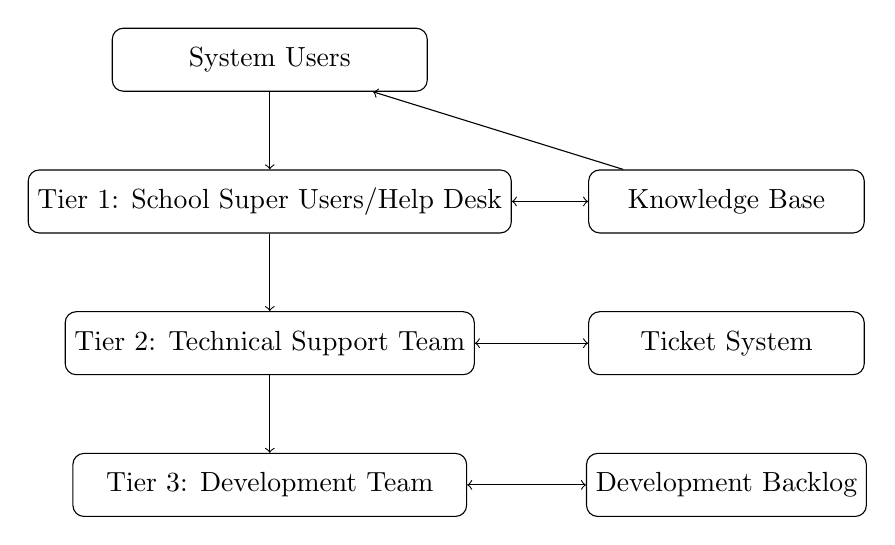
\begin{tikzpicture}[node distance=1.8cm]
\node (user) [rectangle, rounded corners, minimum width=4cm, minimum height=0.8cm, text centered, draw=black] {System Users};

\node (tier1) [rectangle, rounded corners, minimum width=5cm, minimum height=0.8cm, text centered, draw=black, below of=user] {Tier 1: School Super Users/Help Desk};

\node (tier2) [rectangle, rounded corners, minimum width=5cm, minimum height=0.8cm, text centered, draw=black, below of=tier1] {Tier 2: Technical Support Team};

\node (tier3) [rectangle, rounded corners, minimum width=5cm, minimum height=0.8cm, text centered, draw=black, below of=tier2] {Tier 3: Development Team};

\node (kb) [rectangle, rounded corners, minimum width=3.5cm, minimum height=0.8cm, text centered, draw=black, right of=tier1, xshift=4cm] {Knowledge Base};

\node (ticket) [rectangle, rounded corners, minimum width=3.5cm, minimum height=0.8cm, text centered, draw=black, right of=tier2, xshift=4cm] {Ticket System};

\node (dev) [rectangle, rounded corners, minimum width=3.5cm, minimum height=0.8cm, text centered, draw=black, right of=tier3, xshift=4cm] {Development Backlog};

\draw[->] (user) -- (tier1);
\draw[->] (tier1) -- (tier2);
\draw[->] (tier2) -- (tier3);

\draw[<->] (tier1) -- (kb);
\draw[<->] (tier2) -- (ticket);
\draw[<->] (tier3) -- (dev);

\draw[->] (kb) -- (user);

\end{tikzpicture}
\caption{Tiered support model}
\end{figure}

\section{Maintenance Activities}

\begin{table}[H]
\centering
\begin{tabular}{|p{3.5cm}|p{5cm}|p{6cm}|}
\hline
\textbf{Activity Type} & \textbf{Frequency} & \textbf{Description} \\
\hline
Security Updates & Monthly or as needed & \begin{itemize}
\item Dependency vulnerability patching
\item Security hotfixes
\item Regular security scanning
\end{itemize} \\
\hline
Bug Fixes & Bi-weekly releases & \begin{itemize}
\item Addressing reported issues
\item Regression testing
\item Patch releases
\end{itemize} \\
\hline
Feature Enhancements & Quarterly releases & \begin{itemize}
\item New functionality based on feedback
\item User experience improvements
\item Performance optimizations
\end{itemize} \\
\hline
Database Maintenance & Weekly & \begin{itemize}
\item Index optimization
\item Query performance tuning
\item Storage monitoring
\end{itemize} \\
\hline
Backup \& Recovery & Daily with monthly testing & \begin{itemize}
\item Automated backup procedures
\item Disaster recovery testing
\item Data retention management
\end{itemize} \\
\hline
Performance Monitoring & Continuous & \begin{itemize}
\item Response time tracking
\item Resource utilization assessment
\item Bottleneck identification
\end{itemize} \\
\hline
\end{tabular}
\caption{Maintenance activities schedule}
\end{table}

\section{Long-term Evolution}

\begin{itemize}
    \item \textbf{Feedback Collection:} Ongoing gathering of user feedback via surveys, feature requests, and usage analytics.
    
    \item \textbf{Roadmap Development:} Quarterly revision of the product roadmap based on stakeholder needs and technological advancements.
    
    \item \textbf{Major Upgrades:} Annual assessment for major version upgrades with significant feature expansions or architectural improvements.
    
    \item \textbf{Technology Refresh:} Bi-annual evaluation of underlying technologies and frameworks for potential modernization.
    
    \item \textbf{Scaling Strategy:} Continuous monitoring of system usage patterns to anticipate and plan for scaling requirements.
\end{itemize}

\section{Data Flow Overview}

\begin{landscape}
\begin{figure}
\centering
\begin{tikzpicture}[node distance=3cm]
\node (user) [rectangle, rounded corners, minimum width=5cm, minimum height=1cm, text centered, draw=black] {Users (Teachers/Students/Parents)};

\node (ui) [rectangle, rounded corners, minimum width=5cm, minimum height=1cm, text centered, draw=black, below of=user] {User Interface};

\node (online) [diamond, minimum width=3.5cm, minimum height=2cm, text centered, draw=black, below of=ui, yshift=-1cm] {Online?};

\node (direct) [rectangle, rounded corners, minimum width=5cm, minimum height=1cm, text centered, draw=black, below of=online, xshift=-6cm, yshift=-1cm] {Direct API Communication};

\node (offline) [rectangle, rounded corners, minimum width=5cm, minimum height=1cm, text centered, draw=black, below of=online, x\section{Complete Module Structure}

The system is organized into a comprehensive set of functional modules, each responsible for specific aspects of school management:

\begin{figure}[H]
\centering
\begin{tikzpicture}[
  level 1/.style={sibling distance=20mm},
  level 2/.style={sibling distance=15mm},
  edge from parent/.style={draw,->},
  module/.style={rectangle, rounded corners, draw, align=center, minimum height=7mm, minimum width=20mm, font=\footnotesize}
]

% Top level modules
\node[module] (auth) at (0,0) {Authentication \& Authorization};
\node[module] (user) at (2.5,0) {User Management};
\node[module] (dash) at (5,0) {Dashboards};
\node[module] (student) at (7.5,0) {Student Management};
\node[module] (teacher) at (10,0) {Teacher Management};

% Second level modules
\node[module] (login) at (0,-1.5) {User Login, Session Management};
\node[module] (profiles) at (2.5,-1.5) {User Profiles};
\node[module] (admin) at (4,-1.5) {Admin};
\node[module] (teacherdash) at (5,-1.5) {Teacher};
\node[module] (parent) at (6,-1.5) {Parent};
\node[module] (studentdash) at (7,-1.5) {Student};
\node[module] (records) at (8.5,-1.5) {Records};
\node[module] (profile) at (10,-1.5) {Profile};

% Connect modules
\draw[->] (auth) -- (login);
\draw[->] (user) -- (profiles);
\draw[->] (dash) -- (admin);
\draw[->] (dash) -- (teacherdash);
\draw[->] (dash) -- (parent);
\draw[->] (dash) -- (studentdash);
\draw[->] (student) -- (records);
\draw[->] (teacher) -- (profile);

% Additional modules in next row
\node[module] (class) at (0,-3) {Class \& Scheduling};
\node[module] (attend) at (2.5,-3) {Attendance Module};
\node[module] (grade) at (5,-3) {Grading \& Assignments};
\node[module] (msg) at (7.5,-3) {Messaging \& Communication};
\node[module] (pay) at (10,-3) {Payment \& Billing};

% Connect additional modules
\node[module] (timetable) at (0,-4.5) {Timetables};
\node[module] (marking) at (2.5,-4.5) {Marking \& History};
\node[module] (assess) at (5,-4.5) {Assessment};
\node[module] (direct) at (7.5,-4.5) {Direct Messaging};
\node[module] (invoice) at (10,-4.5) {Invoice Generation};

\draw[->] (class) -- (timetable);
\draw[->] (attend) -- (marking);
\draw[->] (grade) -- (assess);
\draw[->] (msg) -- (direct);
\draw[->] (pay) -- (invoice);

% Final row of modules
\node[module] (report) at (0,-6) {Reports \& Analytics};
\node[module] (notif) at (2.5,-6) {Notifications Module};
\node[module] (offline) at (5,-6) {Offline Data Sync};
\node[module] (system) at (7.5,-6) {System Settings};

% Connect final row
\node[module] (analytics) at (0,-7.5) {Academic Analytics};
\node[module] (push) at (2.5,-7.5) {Push Notifications};
\node[module] (storage) at (5,-7.5) {Local Storage};
\node[module] (config) at (7.5,-7.5) {Configuration};

\draw[->] (report) -- (analytics);
\draw[->] (notif) -- (push);
\draw[->] (offline) -- (storage);
\draw[->] (system) -- (config);

\end{tikzpicture}
\caption{Comprehensive module structure of the school management system}
\label{fig:module_structure}
\end{figure}

\section{System Interaction Flow}

The following diagram illustrates how users interact with the system and how data flows between the various modules:

\begin{figure}[H]
\centering
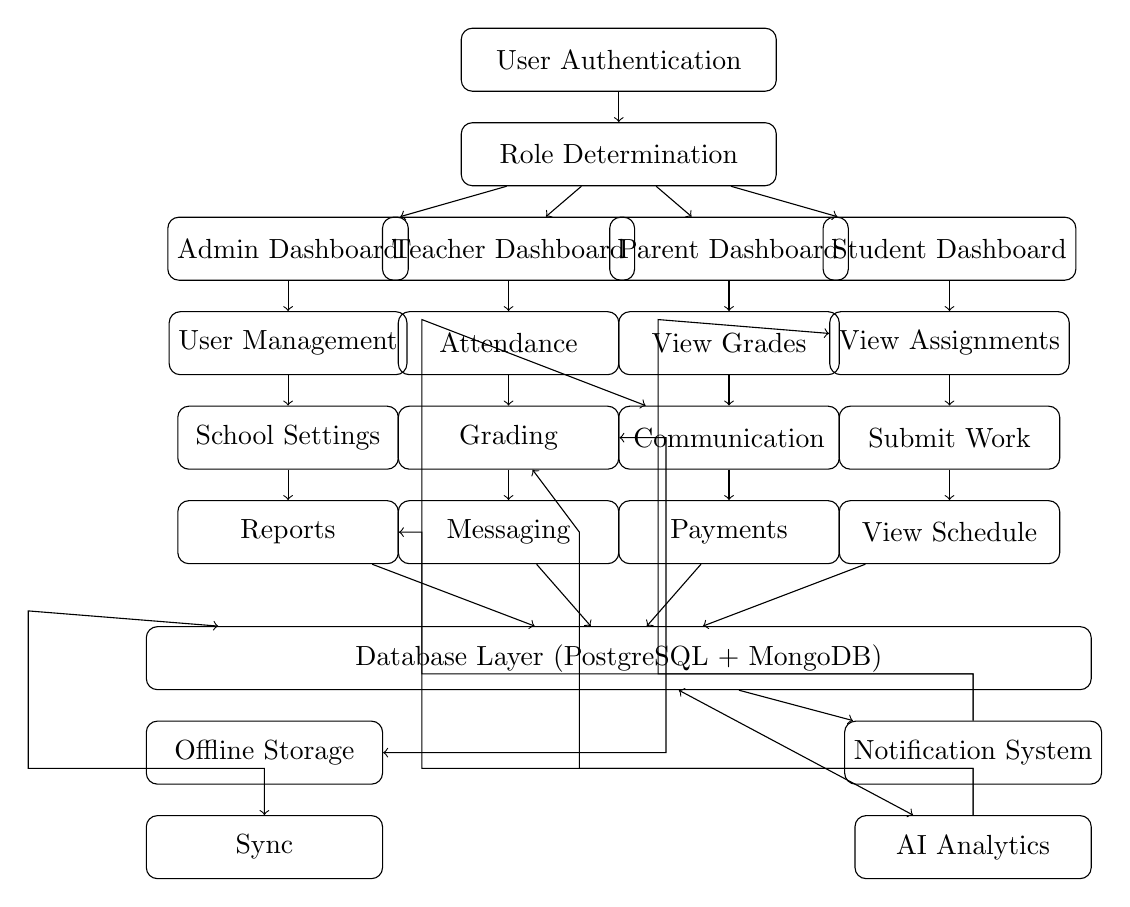
\begin{tikzpicture}[node distance=1.2cm, 
                    every node/.style={rectangle, rounded corners, draw, align=center, 
                                      minimum height=0.8cm}]

% Top row
\node[text centered, minimum width=4cm] (auth) {User Authentication};
\node[text centered, minimum width=4cm, below of=auth] (role) {Role Determination};

% Role-specific dashboards
\node[text centered, minimum width=2.8cm, below of=role, xshift=-4.2cm] (admin) {Admin Dashboard};
\node[text centered, minimum width=2.8cm, below of=role, xshift=-1.4cm] (teacher) {Teacher Dashboard};
\node[text centered, minimum width=2.8cm, below of=role, xshift=1.4cm] (parent) {Parent Dashboard};
\node[text centered, minimum width=2.8cm, below of=role, xshift=4.2cm] (student) {Student Dashboard};

% Action rows for each dashboard
\node[text centered, minimum width=2.8cm, below of=admin] (admin1) {User Management};
\node[text centered, minimum width=2.8cm, below of=admin1] (admin2) {School Settings};
\node[text centered, minimum width=2.8cm, below of=admin2] (admin3) {Reports};

\node[text centered, minimum width=2.8cm, below of=teacher] (teacher1) {Attendance};
\node[text centered, minimum width=2.8cm, below of=teacher1] (teacher2) {Grading};
\node[text centered, minimum width=2.8cm, below of=teacher2] (teacher3) {Messaging};

\node[text centered, minimum width=2.8cm, below of=parent] (parent1) {View Grades};
\node[text centered, minimum width=2.8cm, below of=parent1] (parent2) {Communication};
\node[text centered, minimum width=2.8cm, below of=parent2] (parent3) {Payments};

\node[text centered, minimum width=2.8cm, below of=student] (student1) {View Assignments};
\node[text centered, minimum width=2.8cm, below of=student1] (student2) {Submit Work};
\node[text centered, minimum width=2.8cm, below of=student2] (student3) {View Schedule};

% Database and supporting systems
\node[text centered, minimum width=12cm, below of=admin3, xshift=4.2cm, yshift=-0.4cm] (db) {Database Layer (PostgreSQL + MongoDB)};

\node[text centered, minimum width=3cm, below of=db, xshift=-4.5cm] (offline) {Offline Storage};
\node[text centered, minimum width=3cm, below of=offline] (sync) {Sync};

\node[text centered, minimum width=3cm, below of=db, xshift=4.5cm] (notif) {Notification System};
\node[text centered, minimum width=3cm, below of=notif] (ai) {AI Analytics};

% Connections
\draw[->] (auth) -- (role);
\draw[->] (role) -- (admin);
\draw[->] (role) -- (teacher);
\draw[->] (role) -- (parent);
\draw[->] (role) -- (student);

\draw[->] (admin) -- (admin1);
\draw[->] (admin1) -- (admin2);
\draw[->] (admin2) -- (admin3);

\draw[->] (teacher) -- (teacher1);
\draw[->] (teacher1) -- (teacher2);
\draw[->] (teacher2) -- (teacher3);

\draw[->] (parent) -- (parent1);
\draw[->] (parent1) -- (parent2);
\draw[->] (parent2) -- (parent3);

\draw[->] (student) -- (student1);
\draw[->] (student1) -- (student2);
\draw[->] (student2) -- (student3);

\draw[->] (admin3) -- (db);
\draw[->] (teacher3) -- (db);
\draw[->] (parent3) -- (db);
\draw[->] (student3) -- (db);

\draw[<->] (teacher2) -- ++(2,0) -- ++(0,-4) -- (offline);
\draw[->] (offline) -- (sync);
\draw[->] (sync) -- ++(0,1) -- ++(-3,0) -- ++(0,2) -- (db);

\draw[->] (db) -- (notif);
\draw[->] (notif) -- ++(0,1) -- ++(-7,0) -- ++(0,4.5) -- (parent2);
\draw[->] (notif) -- ++(0,1) -- ++(-4,0) -- ++(0,4.5) -- (student1);

\draw[<->] (db) -- (ai);
\draw[->] (ai) -- ++(0,1) -- ++(-7,0) -- ++(0,3) -- (admin3);
\draw[->] (ai) -- ++(0,1) -- ++(-5,0) -- ++(0,3) -- (teacher2);

\end{tikzpicture}
\caption{System interaction flow showing user roles, actions, and data processing}
\label{fig:system_interaction}
\end{figure}\section{Parent Workflows}

\subsection{Parent Monitoring Child's Progress Workflow}

\begin{figure}[H]
\centering
\resizebox{\textwidth}{!}{
\begin{tikzpicture}[node distance=2.5cm]
\node (login) [rectangle, rounded corners, minimum width=4cm, minimum height=0.8cm, text centered, draw=black] {Parent logs into system};

\node (dashboard) [rectangle, rounded corners, minimum width=4cm, minimum height=0.8cm, text centered, draw=black, below of=login] {Parent views dashboard};

\node (select) [rectangle, rounded corners, minimum width=4cm, minimum height=0.8cm, text centered, draw=black, below of=dashboard] {Parent selects child (if multiple)};

\node (overview) [rectangle, rounded corners, minimum width=4.5cm, minimum height=0.8cm, text centered, draw=black, below of=select] {Parent views child's overview};

\node (decision) [diamond, minimum width=3.2cm, minimum height=1.8cm, text centered, draw=black, below of=overview, yshift=-1.2cm] {Area to\\ Review?};

\node (grades) [rectangle, rounded corners, minimum width=3.5cm, minimum height=0.8cm, text centered, draw=black, below of=decision, xshift=-5.5cm, yshift=-1.2cm] {Academic Performance};

\node (attendance) [rectangle, rounded corners, minimum width=3.5cm, minimum height=0.8cm, text centered, draw=black, below of=decision, yshift=-1.2cm] {Attendance History};

\node (behavior) [rectangle, rounded corners, minimum width=3.5cm, minimum height=0.8cm, text centered, draw=black, below of=decision, xshift=5.5cm, yshift=-1.2cm] {Upcoming Tasks};

\node (grade_detail) [rectangle, rounded corners, minimum width=3.5cm, minimum height=0.8cm, text centered, draw=black, below of=grades, yshift=-0.8cm] {Review grades and feedback};

\node (attend_detail) [rectangle, rounded corners, minimum width=3.5cm, minimum height=0.8cm, text centered, draw=black, below of=attendance, yshift=-0.8cm] {View attendance patterns};

\node (task_detail) [rectangle, rounded corners, minimum width=3.5cm, minimum height=0.8cm, text centered, draw=black, below of=behavior, yshift=-0.8cm] {Check assignments/exams};

\node (contact) [rectangle, rounded corners, minimum width=5cm, minimum height=0.8cm, text centered, draw=black, below of=attend_detail, yshift=-2cm] {Option to contact teacher directly};

\node (download) [rectangle, rounded corners, minimum width=5cm, minimum height=0.8cm, text centered, draw=black, below of=contact, yshift=-0.8cm] {Download/print reports if needed};

\draw[->] (login) -- (dashboard);
\draw[->] (dashboard) -- (select);
\draw[->] (select) -- (overview);
\draw[->] (overview) -- (decision);
\draw[->] (decision) -- (grades) node[midway, above, sloped] {Grades};
\draw[->] (decision) -- (attendance) node[midway, above] {Attendance};
\draw[->] (decision) -- (behavior) node[midway, above, sloped] {Tasks};
\draw[->] (grades) -- (grade_detail);
\draw[->] (attendance) -- (attend_detail);
\draw[->] (behavior) -- (task_detail);
\draw[->] (grade_detail) |- (contact);
\draw[->] (attend_detail) -- (contact);
\draw[->] (task_detail) |- (contact);
\draw[->] (contact) -- (download);
\end{tikzpicture}
}
\caption{Parent workflow for monitoring child's progress}
\end{figure}

\subsection{Parent Communication Workflow}

\begin{figure}[H]
\centering
\resizebox{\textwidth}{!}{
\begin{tikzpicture}[node distance=2.5cm]
\node (login) [rectangle, rounded corners, minimum width=4cm, minimum height=0.8cm, text centered, draw=black] {Parent logs into system};

\node (dashboard) [rectangle, rounded corners, minimum width=4cm, minimum height=0.8cm, text centered, draw=black, below of=login] {Parent views dashboard};

\node (child) [rectangle, rounded corners, minimum width=4cm, minimum height=0.8cm, text centered, draw=black, below of=dashboard] {Parent selects child (if multiple)};

\node (decision) [diamond, minimum width=3.5cm, minimum height=1.8cm, text centered, draw=black, below of=child, yshift=-1.2cm] {Communication\\ Type?};

\node (teacher) [rectangle, rounded corners, minimum width=4cm, minimum height=0.8cm, text centered, draw=black, below of=decision, xshift=-5cm, yshift=-1.2cm] {Message Teacher};

\node (admin) [rectangle, rounded corners, minimum width=4cm, minimum height=0.8cm, text centered, draw=black, below of=decision, xshift=5cm, yshift=-1.2cm] {Contact Administration};

\node (compose) [rectangle, rounded corners, minimum width=4cm, minimum height=0.8cm, text centered, draw=black, below of=teacher, yshift=-0.8cm] {Compose message};

\node (admin_form) [rectangle, rounded corners, minimum width=4cm, minimum height=0.8cm, text centered, draw\section{Parent Workflows}

\subsection{Parent Monitoring Child's Progress Workflow}

\begin{figure}[H]
\centering
\begin{tikzpicture}[node distance=2cm]
\node (login) [rectangle, rounded corners, minimum width=4cm, minimum height=0.8cm, text centered, draw=black] {Parent logs into system};

\node (dashboard) [rectangle, rounded corners, minimum width=4cm, minimum height=0.8cm, text centered, draw=black, below of=login] {Parent views dashboard};

\node (select) [rectangle, rounded corners, minimum width=4cm, minimum height=0.8cm, text centered, draw=black, below of=dashboard] {Parent selects child (if multiple)};

\node (overview) [rectangle, rounded corners, minimum width=4.5cm, minimum height=0.8cm, text centered, draw=black, below of=select] {Parent views child's overview};

\node (decision) [diamond, minimum width=3.2cm, minimum height=1.8cm, text centered, draw=black, below of=overview, yshift=-1.2cm] {Area to\\ Review?};

\node (grades) [rectangle, rounded corners, minimum width=3.5cm, minimum height=0.8cm, text centered, draw=black, below of=decision, xshift=-5.5cm, yshift=-1.2cm] {Academic Performance};

\node (attendance) [rectangle, rounded corners, minimum width=3.5cm, minimum height=0.8cm, text centered, draw=black, below of=decision, yshift=-1.2cm] {Attendance History};

\node (behavior) [rectangle, rounded corners, minimum width=3.5cm, minimum height=0.8cm, text centered, draw=black, below of=decision, xshift=5.5cm, yshift=-1.2cm] {Upcoming Tasks};

\node (grade_detail) [rectangle, rounded corners, minimum width=3.5cm, minimum height=0.8cm, text centered, draw=black, below of=grades, yshift=-0.8cm] {Review grades and feedback};

\node (attend_detail) [rectangle, rounded corners, minimum width=3.5cm, minimum height=0.8cm, text centered, draw=black, below of=attendance, yshift=-0.8cm] {View attendance patterns};

\node (task_detail) [rectangle, rounded corners, minimum width=3.5cm, minimum height=0.8cm, text centered, draw=black, below of=behavior, yshift=-0.8cm] {Check assignments/exams};

\node (contact) [rectangle, rounded corners, minimum width=5cm, minimum height=0.8cm, text centered, draw=black, below of=attend_detail, yshift=-2cm] {Option to contact teacher directly};

\node (download) [rectangle, rounded corners, minimum width=5cm, minimum height=0.8cm, text centered, draw=black, below of=contact, yshift=-0.8cm] {Download/print reports if needed};

\draw[->] (login) -- (dashboard);
\draw[->] (dashboard) -- (select);
\draw[->] (select) -- (overview);
\draw[->] (overview) -- (decision);
\draw[->] (decision) -- (grades) node[midway, above, sloped] {Grades};
\draw[->] (decision) -- (attendance) node[midway, above] {Attendance};
\draw[->] (decision) -- (behavior) node[midway, above, sloped] {Tasks};
\draw[->] (grades) -- (grade_detail);
\draw[->] (attendance) -- (attend_detail);
\draw[->] (behavior) -- (task_detail);
\draw[->] (grade_detail) |- (contact);
\draw[->] (attend_detail) -- (contact);
\draw[->] (task_detail) |- (contact);
\draw[->] (contact) -- (download);

\end{tikzpicture}
\caption{Parent workflow for monitoring child's progress}
\end{figure}

\subsection{Parent Communication Workflow}

\begin{figure}[H]
\centering
\begin{tikzpicture}[node distance=2cm]
\node (login) [rectangle, rounded corners, minimum width=4cm, minimum height=0.8cm, text centered, draw=black] {Parent logs into system};

\node (dashboard) [rectangle, rounded corners, minimum width=4cm, minimum height=0.8cm, text centered, draw=black, below of=login] {Parent views dashboard};

\node (child) [rectangle, rounded corners, minimum width=4cm, minimum height=0.8cm, text centered, draw=black, below of=dashboard] {Parent selects child (if multiple)};

\node (decision) [diamond, minimum width=3.5cm, minimum height=1.8cm, text centered, draw=black, below of=child, yshift=-1.2cm] {Communication\\ Type?};

\node (teacher) [rectangle, rounded corners, minimum width=4cm, minimum height=0.8cm, text centered, draw=black, below of=decision, xshift=-5cm, yshift=-1.2cm] {Message Teacher};

\node (admin) [rectangle, rounded corners, minimum width=4cm, minimum height=0.8cm, text centered, draw=black, below of=decision, xshift=5cm, yshift=-1.2cm] {Contact Administration};

\node (compose) [rectangle, rounded corners, minimum width=4cm, minimum height=0.8cm, text centered, draw=black, below of=teacher, yshift=-0.8cm] {Compose message};

\node (admin_form) [rectangle, rounded corners, minimum width=4cm, minimum height=0.8cm, text centered, draw=black, below of=admin, yshift=-0.8cm] {Fill contact form};

\node (topics) [rectangle, rounded corners, minimum width=5cm, minimum height=1.5cm, text centered, draw=black, below of=compose, yshift=-0.8cm] {- Attendance issues\\ - Academic performance\\ - Assignment clarifications};

\node (admin_topics) [rectangle, rounded corners, minimum width=5cm, minimum height=1.5cm, text centered, draw=black, below of=admin_form, yshift=-0.8cm] {- Administrative requests\\ - Account issues\\ - General feedback};

\node (follow_up) [rectangle, rounded corners, minimum width=6cm, minimum height=0.8cm, text centered, draw=black, below of=topics, xshift=2.5cm, yshift=-2cm] {Parent receives notification when response arrives};

\node (history) [rectangle, rounded corners, minimum width=6cm, minimum height=0.8cm, text centered, draw=black, below of=follow_up, yshift=-0.8cm] {Communication history available for reference};

\draw[->] (login) -- (dashboard);
\draw[->] (dashboard) -- (child);
\draw[->] (child) -- (decision);
\draw[->] (decision) -- (teacher) node[midway, above, sloped] {Teacher};
\draw[->] (decision) -- (admin) node[midway, above, sloped] {Administration};
\draw[->] (teacher) -- (compose);
\draw[->] (admin) -- (admin_form);
\draw[->] (compose) -- (topics);
\draw[->] (admin_form) -- (admin_topics);
\draw[->] (topics) |- (follow_up);
\draw[->] (admin_topics) |- (follow_up);
\draw[->] (follow_up) -- (history);

\end{tikzpicture}
\caption{Parent communication workflow}
\end{figure}

\section{System Integration Flow}

\begin{landscape}
\begin{figure}
\centering
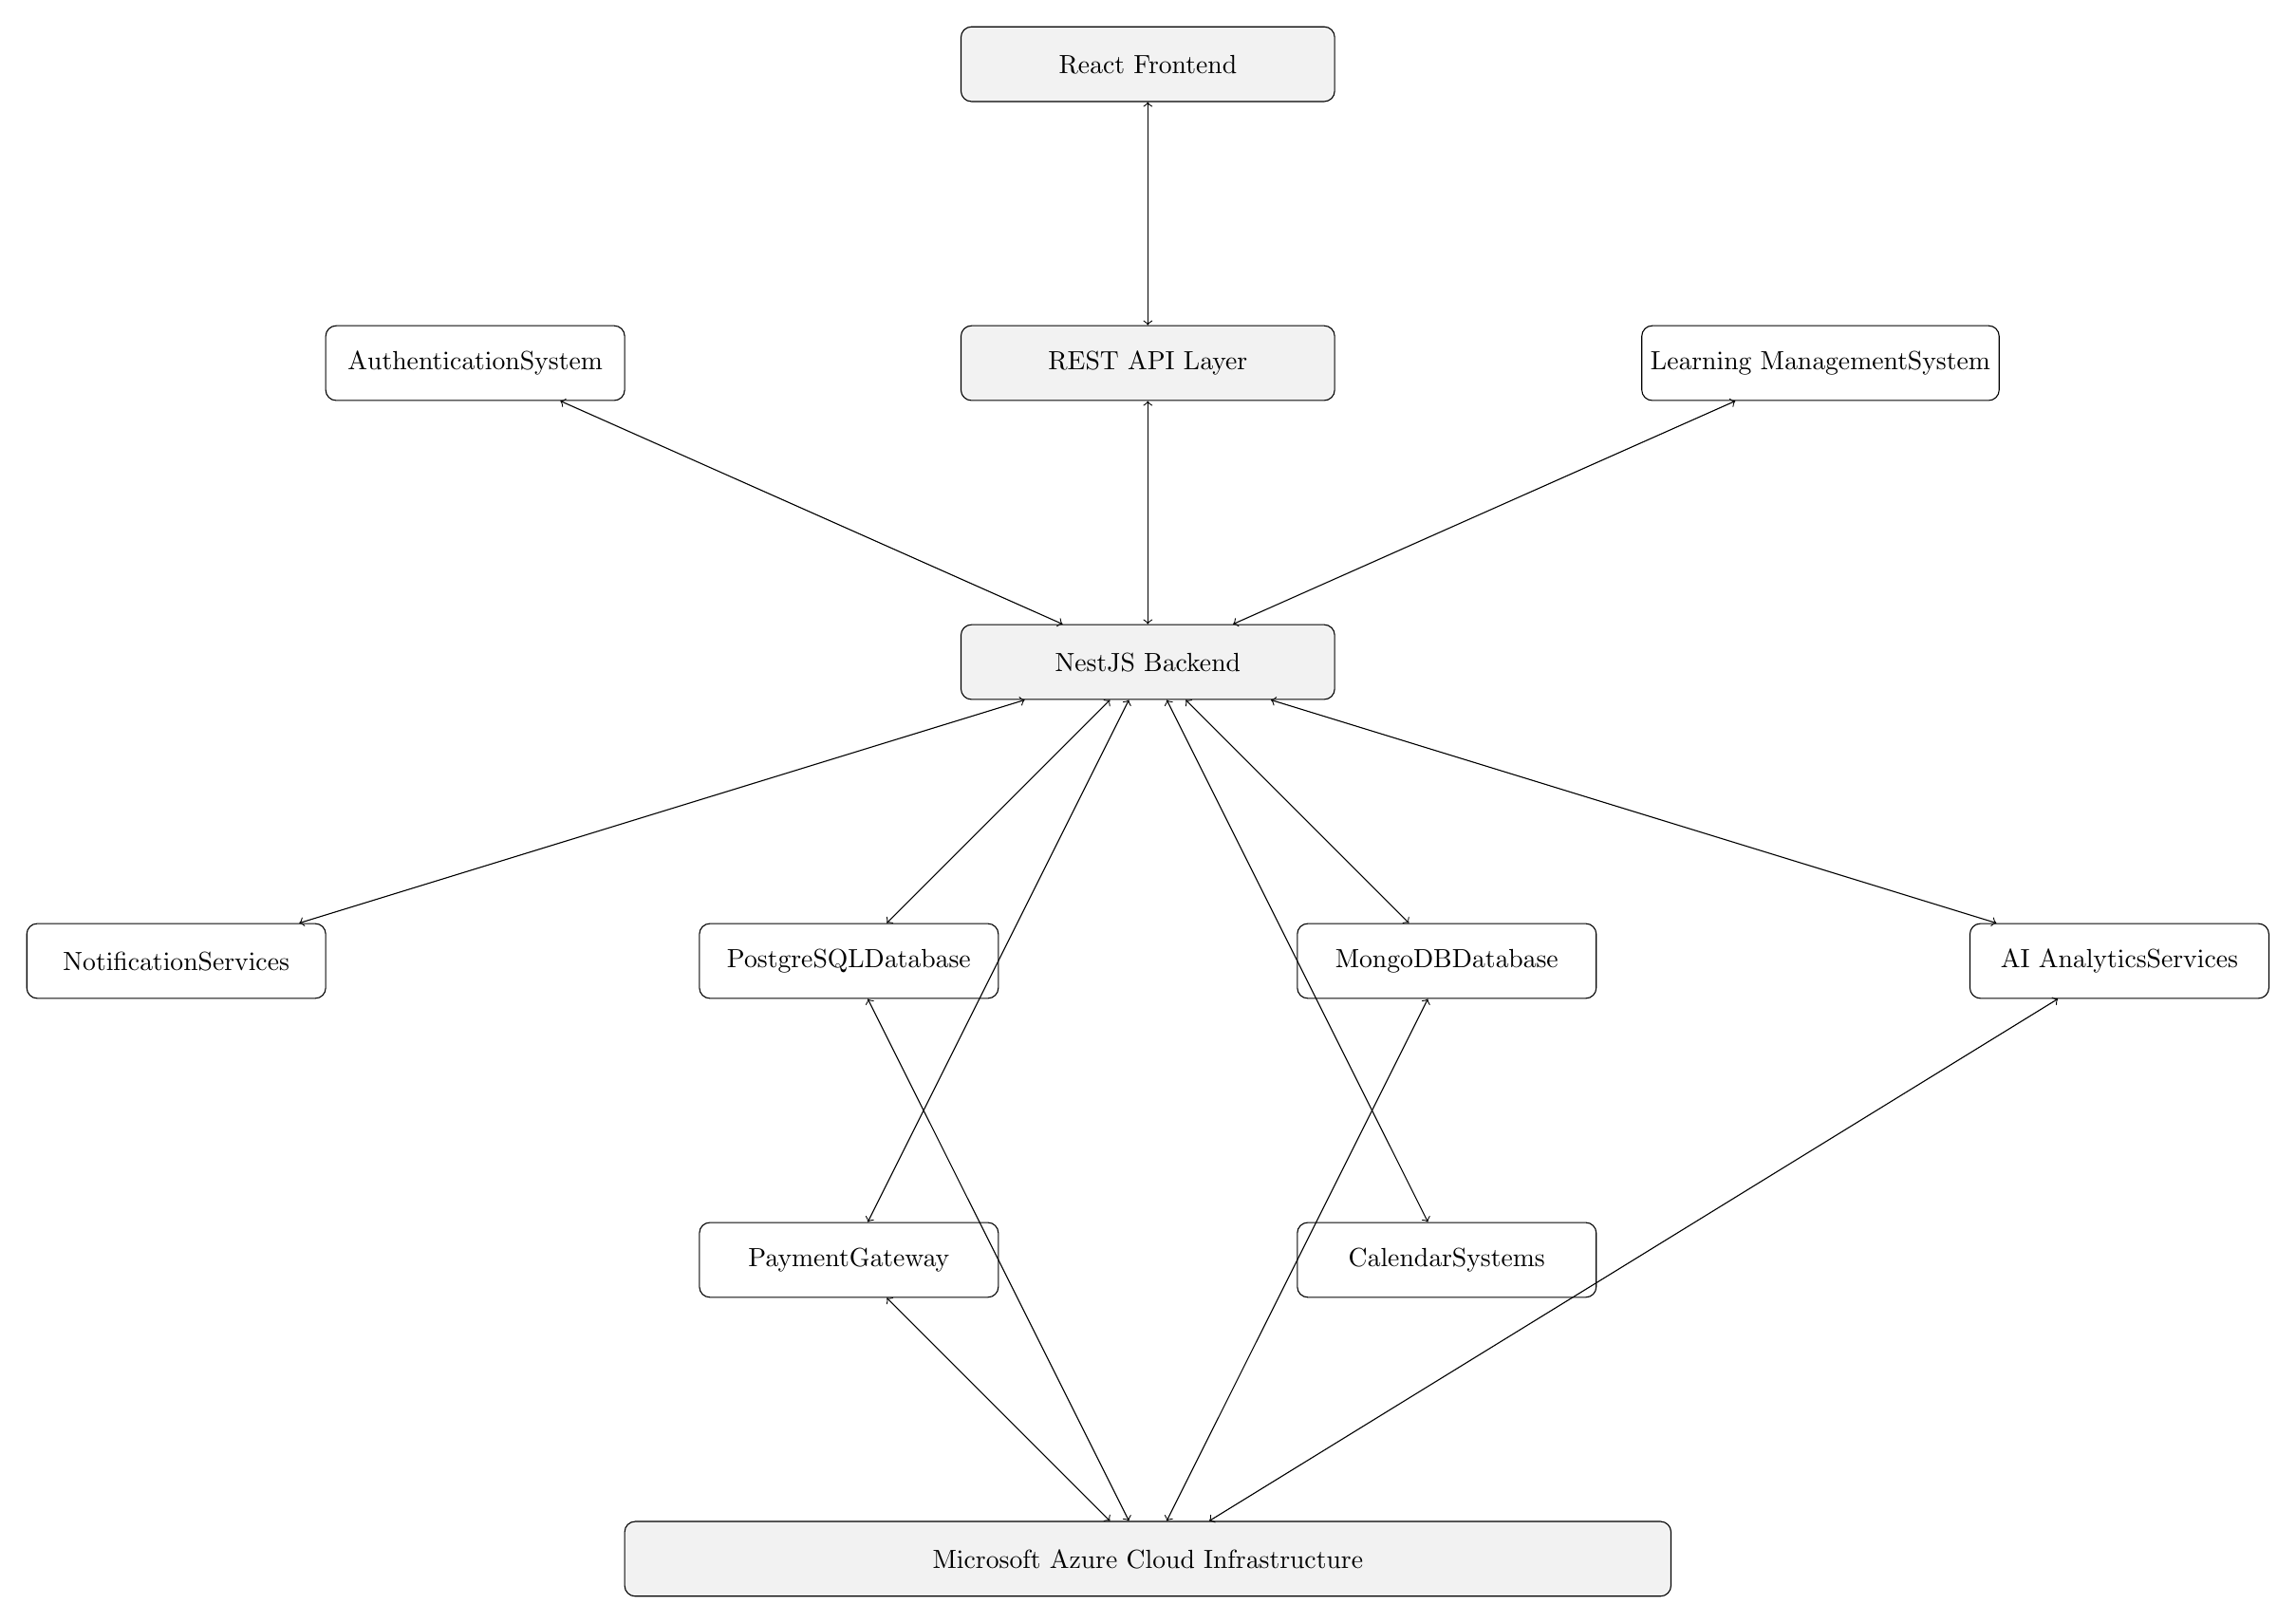
\begin{tikzpicture}[node distance=3cm]
\node (frontend) [rectangle, rounded corners, minimum width=5cm, minimum height=1cm, text centered, draw=black, fill=gray!10] {React Frontend};

\node (api) [rectangle, rounded corners, minimum width=5cm, minimum height=1cm, text centered, draw=black, fill=gray!10, below of=frontend, yshift=-1cm] {REST API Layer};

\node (backend) [rectangle, rounded corners, minimum width=5cm, minimum height=1cm, text centered, draw=black, fill=gray!10, below of=api, yshift=-1cm] {NestJS Backend};

\node (auth) [rectangle, rounded corners, minimum width=4cm, minimum height=1cm, text centered, draw=black, left of=api, xshift=-6cm] {Authentication\\ System};

\node (lms) [rectangle, rounded corners, minimum width=4cm, minimum height=1cm, text centered, draw=black, right of=api, xshift=6cm] {Learning Management\\ System};

\node (postgres) [rectangle, rounded corners, minimum width=4cm, minimum height=1cm, text centered, draw=black, below of=backend, xshift=-4cm, yshift=-1cm] {PostgreSQL\\ Database};

\node (mongodb) [rectangle, rounded corners, minimum width=4cm, minimum height=1cm, text centered, draw=black, below of=backend, xshift=4cm, yshift=-1cm] {MongoDB\\ Database};

\node (notification) [rectangle, rounded corners, minimum width=4cm, minimum height=1cm, text centered, draw=black, left of=postgres, xshift=-6cm] {Notification\\ Services};

\node (ai) [rectangle, rounded corners, minimum width=4cm, minimum height=1cm, text centered, draw=black, right of=mongodb, xshift=6cm] {AI Analytics\\ Services};

\node (payment) [rectangle, rounded corners, minimum width=4cm, minimum height=1cm, text centered, draw=black, below of=postgres, yshift=-1cm] {Payment\\ Gateway};

\node (calendar) [rectangle, rounded corners, minimum width=4cm, minimum height=1cm, text centered, draw=black, below of=mongodb, yshift=-1cm] {Calendar\\ Systems};

\node (cloud) [rectangle, rounded corners, minimum width=14cm, minimum height=1cm, text centered, draw=black, fill=gray!10, below of=payment, xshift=4cm, yshift=-1cm] {Microsoft Azure Cloud Infrastructure};

\draw[<->] (frontend) -- (api);
\draw[<->] (api) -- (backend);
\draw[<->] (backend) -- (postgres);
\draw[<->] (backend) -- (mongodb);
\draw[<->] (backend) -- (auth);
\draw[<->] (backend) -- (lms);
\draw[<->] (backend) -- (notification);
\draw[<->] (backend) -- (ai);
\draw[<->] (backend) -- (payment);
\draw[<->] (backend) -- (calendar);
\draw[<->] (postgres) -- (cloud);
\draw[<->] (mongodb) -- (cloud);
\draw[<->] (payment) -- (cloud);
\draw[<->] (ai) -- (cloud);

\end{tikzpicture}
\caption{System integration flow with external services}
\end{figure}
\end{landscape}

\section{Data Flow Overview}

\begin{landscape}
\begin{figure}
\centering
\begin{tikzpicture}[node distance=3cm]
\node (user) [rectangle, rounded corners, minimum width=5cm, minimum height=1cm, text centered, draw=black] {Users (Teachers/Students/Parents)};

\node (ui) [rectangle, rounded corners, minimum width=5cm, minimum height=1cm, text centered, draw=black, below of=user] {User Interface};

\node (online) [diamond, minimum width=3.5cm, minimum height=2cm, text centered, draw=black, below of=ui, yshift=-1cm] {Online?};

\node (direct) [rectangle, rounded corners, minimum width=5cm, minimum height=1cm, text centered, draw=black, below of=online, xshift=-6cm, yshift=-1cm] {Direct API Communication};

\node (offline) [rectangle, rounded corners, minimum width=5cm, minimum height=1cm, text centered, draw=black, below of=online, xshift=6cm, yshift=-1cm] {Offline Storage (IndexedDB)};

\node (api) [rectangle, rounded corners, minimum width=5cm, minimum height=1cm, text centered, draw=black, below of=direct, yshift=-1cm] {API Gateway Layer};

\node (sync) [rectangle, rounded corners, minimum width=5cm, minimum height=1cm, text centered, draw=black, below of=offline, yshift=-1cm] {Background Sync};

\node (business) [rectangle, rounded corners, minimum width=7cm, minimum height=1cm, text centered, draw=black, below of=api, xshift=3cm, yshift=-1cm] {Business Logic Layer};

\node (data) [rectangle, rounded corners, minimum width=7cm, minimum height=1cm, text centered, draw=black, below of=business, yshift=-1cm] {Data Access Layer};

\node (sql) [rectangle, rounded corners, minimum width=5cm, minimum height=1cm, text centered, draw=black, below of=data, xshift=-4cm, yshift=-1cm] {PostgreSQL\\ (Core Data)};

\node (nosql) [rectangle, rounded corners, minimum width=5cm, minimum height=1cm, text centered, draw=black, below of=data, xshift=4cm, yshift=-1cm] {MongoDB\\ (Analytics/Logs)};

\node (analytics) [rectangle, rounded corners, minimum width=5cm, minimum height=1cm, text centered, draw=black, right of=business, xshift=6cm] {Analytics Engine};

\node (notifications) [rectangle, rounded corners, minimum width=5cm, minimum height=1cm, text centered, draw=black, left of=business, xshift=-6cm] {Notification Service};

\draw[->] (user) -- (ui);
\draw[->] (ui) -- (online);
\draw[->] (online) -- (direct) node[midway, above, sloped] {Yes};
\draw[->] (online) -- (offline) node[midway, above, sloped] {No};
\draw[->] (direct) -- (api);
\draw[->] (offline) -- (sync);
\draw[->] (sync) |- (api);
\draw[->] (api) -- (business);
\draw[->] (business) -- (data);
\draw[->] (data) -- (sql);
\draw[->] (data) -- (nosql);
\draw[<->] (business) -- (analytics);
\draw[<->] (business) -- (notifications);
\draw[->] (notifications) -| (user);
\draw[->] (analytics) -- (nosql);

\end{tikzpicture}
\caption{Data flow overview with online and offline paths}
\end{figure}
\end{landscape}\section{Student Workflows}

\subsection{Student Assignment Submission Workflow}

\begin{figure}[H]
\centering
\begin{tikzpicture}[node distance=2cm]
\node (login) [rectangle, rounded corners, minimum width=4cm, minimum height=0.8cm, text centered, draw=black] {Student logs into system};

\node (dashboard) [rectangle, rounded corners, minimum width=4cm, minimum height=0.8cm, text centered, draw=black, below of=login] {Student views dashboard};

\node (assignments) [rectangle, rounded corners, minimum width=4cm, minimum height=0.8cm, text centered, draw=black, below of=dashboard] {Student opens Assignments section};

\node (view) [rectangle, rounded corners, minimum width=4.5cm, minimum height=0.8cm, text centered, draw=black, below of=assignments] {Student views assignment details};

\node (work) [rectangle, rounded corners, minimum width=4.5cm, minimum height=0.8cm, text centered, draw=black, below of=view] {Student completes assignment offline};

\node (upload) [rectangle, rounded corners, minimum width=4cm, minimum height=0.8cm, text centered, draw=black, below of=work] {Student uploads work to system};

\node (decision) [diamond, minimum width=2.5cm, minimum height=1.5cm, text centered, draw=black, below of=upload, yshift=-1.2cm] {Online?};

\node (submit_online) [rectangle, rounded corners, minimum width=4cm, minimum height=0.8cm, text centered, draw=black, below of=decision, xshift=-4.5cm, yshift=-1.2cm] {Work submitted directly};

\node (store_offline) [rectangle, rounded corners, minimum width=4cm, minimum height=0.8cm, text centered, draw=black, below of=decision, xshift=4.5cm, yshift=-1.2cm] {Work stored locally in browser};

\node (confirm_online) [rectangle, rounded corners, minimum width=4cm, minimum height=0.8cm, text centered, draw=black, below of=submit_online, yshift=-0.8cm] {System confirms submission};

\node (sync) [rectangle, rounded corners, minimum width=4cm, minimum height=0.8cm, text centered, draw=black, below of=store_offline, yshift=-0.8cm] {Auto-sync when online again};

\node (teacher) [rectangle, rounded corners, minimum width=5cm, minimum height=0.8cm, text centered, draw=black, below of=confirm_online, yshift=-1.8cm] {Assignment available for teacher review};

\node (feedback) [rectangle, rounded corners, minimum width=5cm, minimum height=0.8cm, text centered, draw=black, below of=teacher, yshift=-0.8cm] {Student later receives grade and feedback};

\draw[->] (login) -- (dashboard);
\draw[->] (dashboard) -- (assignments);
\draw[->] (assignments) -- (view);
\draw[->] (view) -- (work);
\draw[->] (work) -- (upload);
\draw[->] (upload) -- (decision);
\draw[->] (decision) -- (submit_online) node[midway, above, sloped] {Yes};
\draw[->] (decision) -- (store_offline) node[midway, above, sloped] {No};
\draw[->] (submit_online) -- (confirm_online);
\draw[->] (store_offline) -- (sync);
\draw[->] (confirm_online) -- (teacher);
\draw[->] (sync) |- (teacher);
\draw[->] (teacher) -- (feedback);

\end{tikzpicture}
\caption{Student workflow for assignment submission}
\end{figure}

\subsection{Student Schedule and Grades Review Workflow}

\begin{figure}[H]
\centering
\begin{tikzpicture}[node distance=2cm]
\node (login) [rectangle, rounded corners, minimum width=4cm, minimum height=0.8cm, text centered, draw=black] {Student logs into system};

\node (dashboard) [rectangle, rounded corners, minimum width=4cm, minimum height=0.8cm, text centered, draw=black, below of=login] {Student views dashboard};

\node (decision) [diamond, minimum width=3.2cm, minimum height=1.8cm, text centered, draw=black, below of=dashboard, yshift=-1.2cm] {Information\\ to View?};

\node (schedule) [rectangle, rounded corners, minimum width=3.5cm, minimum height=0.8cm, text centered, draw=black, below of=decision, xshift=-5cm, yshift=-1.2cm] {Class Schedule};

\node (grades) [rectangle, rounded corners, minimum width=3.5cm, minimum height=0.8cm, text centered, draw=black, below of=decision, yshift=-1.2cm] {Academic Grades};

\node (tasks) [rectangle, rounded corners, minimum width=3.5cm, minimum height=0.8cm, text centered, draw=black, below of=decision, xshift=5cm, yshift=-1.2cm] {Upcoming Tasks};

\node (view_schedule) [rectangle, rounded corners, minimum width=3.5cm, minimum height=0.8cm, text centered, draw=black, below of=schedule, yshift=-0.8cm] {Daily/weekly timetable};

\node (view_grades) [rectangle, rounded corners, minimum width=3.5cm, minimum height=0.8cm, text centered, draw=black, below of=grades, yshift=-0.8cm] {Subject-wise performance};

\node (view_tasks) [rectangle, rounded corners, minimum width=3.5cm, minimum height=0.8cm, text centered, draw=black, below of=tasks, yshift=-0.8cm] {Assignments/test dates};

\node (detail) [rectangle, rounded corners, minimum width=5cm, minimum height=0.8cm, text centered, draw=black, below of=view_grades, yshift=-1.8cm] {Student can drill down for details};

\node (action) [rectangle, rounded corners, minimum width=5.5cm, minimum height=0.8cm, text centered, draw=black, below of=detail, yshift=-0.8cm] {Student can take appropriate actions based on data};

\node (offline) [rectangle, rounded corners, minimum width=5cm, minimum height=0.8cm, text centered, draw=black, below of=action, yshift=-0.8cm] {Information available offline if previously loaded};

\draw[->] (login) -- (dashboard);
\draw[->] (dashboard) -- (decision);
\draw[->] (decision) -- (schedule) node[midway, above, sloped] {Schedule};
\draw[->] (decision) -- (grades) node[midway, above] {Grades};
\draw[->] (decision) -- (tasks) node[midway, above, sloped] {Tasks};
\draw[->] (schedule) -- (view_schedule);
\draw[->] (grades) -- (view_grades);
\draw[->] (tasks) -- (view_tasks);
\draw[->] (view_schedule) |- (detail);
\draw[->] (view_grades) -- (detail);
\draw[->] (view_tasks) |- (detail);
\draw[->] (detail) -- (action);
\draw[->] (action) -- (offline);

\end{tikzpicture}
\caption{Student workflow for schedule and grades review}
\end{figure}\chapter{Key Implementation Challenges \& Mitigation Strategies}

During the implementation of the school management system, several technical and organizational challenges are anticipated. This section outlines these challenges and provides strategies to address them effectively.

\section{Technical Challenges}

\begin{table}[H]
\centering
\begin{tabular}{|p{3.5cm}|p{5.5cm}|p{5.5cm}|}
\hline
\textbf{Challenge} & \textbf{Description} & \textbf{Mitigation Strategy} \\
\hline
Data Migration & Transferring existing student, teacher, and academic records from legacy systems & \begin{itemize}
\item Develop specialized ETL scripts
\item Implement a phased migration approach
\item Provide a transitional period with both systems
\end{itemize} \\
\hline
Offline Reliability & Ensuring data integrity during offline usage and synchronization & \begin{itemize}
\item Robust conflict resolution mechanisms
\item Clear timestamp-based precedence rules
\item Comprehensive sync status indicators
\end{itemize} \\
\hline
Performance at Scale & Maintaining responsive performance with large datasets and concurrent users & \begin{itemize}
\item Implement database indexing strategies
\item Use caching for frequently accessed data
\item Design for horizontal scalability on Azure
\end{itemize} \\
\hline
AI Model Accuracy & Building accurate prediction and facial recognition models & \begin{itemize}
\item Start with conservative, high-confidence predictions
\item Continuously improve models with new data
\item Provide manual override options
\end{itemize} \\
\hline
Security & Protecting sensitive student data and preventing unauthorized access & \begin{itemize}
\item Regular security audits and penetration testing
\item End-to-end encryption for sensitive data
\item Comprehensive role-based access controls
\end{itemize} \\
\hline
\end{tabular}
\caption{Technical implementation challenges and mitigation strategies}
\end{table}

\section{Organizational Challenges}

\begin{table}[H]
\centering
\begin{tabular}{|p{3.5cm}|p{5.5cm}|p{5.5cm}|}
\hline
\textbf{Challenge} & \textbf{Description} & \textbf{Mitigation Strategy} \\
\hline
User Adoption & Ensuring stakeholders embrace and effectively use the new system & \begin{itemize}
\item Comprehensive training program
\item Intuitive UX design for minimal learning curve
\item Designated "super users" within each user group
\end{itemize} \\
\hline
Changing Requirements & Managing evolving requirements during implementation & \begin{itemize}
\item Agile methodology for adaptability
\item Regular stakeholder feedback sessions
\item Modular design for feature flexibility
\end{itemize} \\
\hline
Training & Educating staff, parents, and students on system usage & \begin{itemize}
\item Role-specific training materials and videos
\item In-app guided tours and contextual help
\item Support desk during initial deployment
\end{itemize} \\
\hline
Workflow Integration & Adapting the system to existing school processes & \begin{itemize}
\item Process mapping workshops before implementation
\item Configurable workflows in the system
\item Phased approach to process changes
\end{itemize} \\
\hline
Stakeholder Alignment & Managing expectations across diverse stakeholder groups & \begin{itemize}
\item Regular progress updates and demos
\item Clear communication about features and limitations
\item Feedback channels for continuous improvement
\end{itemize} \\
\hline
\end{tabular}
\caption{Organizational implementation challenges and mitigation strategies}
\end{table}

\chapter{Data Security \& Compliance}

Protecting sensitive student and academic data is a critical aspect of the school management system implementation. This section outlines the comprehensive security measures and compliance considerations incorporated into the design.

\section{Security Architecture}

\begin{figure}[H]
\centering
\begin{tikzpicture}[node distance=1.8cm]
\node (user) [rectangle, rounded corners, minimum width=4cm, minimum height=0.8cm, text centered, draw=black] {User};

\node (auth) [rectangle, rounded corners, minimum width=4cm, minimum height=0.8cm, text centered, draw=black, below of=user] {Authentication Layer};

\node (jwt) [rectangle, rounded corners, minimum width=4cm, minimum height=0.8cm, text centered, draw=black, below of=auth] {JWT Token Validation};

\node (rbac) [rectangle, rounded corners, minimum width=4cm, minimum height=0.8cm, text centered, draw=black, below of=jwt] {Role-Based Access Control};

\node (api) [rectangle, rounded corners, minimum width=4cm, minimum height=0.8cm, text centered, draw=black, below of=rbac] {API Security Middleware};

\node (business) [rectangle, rounded corners, minimum width=4cm, minimum height=0.8cm, text centered, draw=black, below of=api] {Business Logic Layer};

\node (data) [rectangle, rounded corners, minimum width=4cm, minimum height=0.8cm, text centered, draw=black, below of=business] {Data Access Layer};

\node (encryption) [rectangle, rounded corners, minimum width=4cm, minimum height=0.8cm, text centered, draw=black, below of=data] {Data Encryption};

\node (database) [rectangle, rounded corners, minimum width=4cm, minimum height=0.8cm, text centered, draw=black, below of=encryption] {Database Storage};

\node (logging) [rectangle, rounded corners, minimum width=4cm, minimum height=0.8cm, text centered, draw=black, right of=data, xshift=5cm] {Security Audit Logging};

\node (monitoring) [rectangle, rounded corners, minimum width=4cm, minimum height=0.8cm, text centered, draw=black, below of=logging] {Threat Monitoring};

\draw[->] (user) -- (auth);
\draw[->] (auth) -- (jwt);
\draw[->] (jwt) -- (rbac);
\draw[->] (rbac) -- (api);
\draw[->] (api) -- (business);
\draw[->] (business) -- (data);
\draw[->] (data) -- (encryption);
\draw[->] (encryption) -- (database);
\draw[->] (api) -- (logging);
\draw[->] (data) -- (logging);
\draw[->] (logging) -- (monitoring);

\end{tikzpicture}
\caption{Security architecture of the school management system}
\end{figure}

\section{Security Measures}

\begin{itemize}
    \item \textbf{Authentication:} Multi-factor authentication for administrative accounts, strong password policies, and secure password reset mechanisms.
    
    \item \textbf{Authorization:} Granular role-based access control ensuring users only access data appropriate to their role.
    
    \item \textbf{Data Encryption:} All sensitive data encrypted both in transit (HTTPS/TLS) and at rest (AES-256 encryption).
    
    \item \textbf{Secure APIs:} API endpoints protected against common vulnerabilities (injection, XSS, CSRF) with input validation and sanitization.
    
    \item \textbf{Audit Logging:} Comprehensive logging of all security-relevant events and access to sensitive data.
    
    \item \textbf{Regular Security Testing:} Scheduled penetration testing and vulnerability assessments.
    
    \item \textbf{Secure Development:} Following secure coding practices and regular dependency vulnerability scanning.
    
    \item \textbf{Data Minimization:} Collecting and storing only necessary data to reduce exposure risk.
\end{itemize}

\section{Compliance Considerations}

\begin{table}[H]
\centering
\begin{tabular}{|p{3cm}|p{11.5cm}|}
\hline
\textbf{Regulation} & \textbf{Implementation Approach} \\
\hline
FERPA (USA) & \begin{itemize}
\item Parental consent for sharing student information
\item Audit trails for all data access
\item Strict access controls limiting data visibility
\item Ability to generate compliance reports
\end{itemize} \\
\hline
GDPR (EU) & \begin{itemize}
\item Data processing consent management
\item Right to access, rectification, and erasure mechanisms
\item Data breach notification capabilities
\item Data retention policies and automated purging
\end{itemize} \\
\hline
COPPA (USA) & \begin{itemize}
\item Age verification for student accounts
\item Parental consent management
\item Limited data collection from minors
\item Simplified privacy notices
\end{itemize} \\
\hline
Local Education Laws & \begin{itemize}
\item Configurable data retention policies
\item Compliance reporting capabilities
\item Adaptable privacy controls for regional requirements
\end{itemize} \\
\hline
\end{tabular}
\caption{Compliance considerations and implementation approaches}
\end{table}

\chapter{Training \& Adoption Strategy}

A comprehensive training and adoption strategy is essential for successful implementation of the school management system. This section outlines the approach to ensure all stakeholders can effectively use the system.

\section{Training Approach}

\begin{figure}[H]
\centering
\begin{tikzpicture}[node distance=1.8cm]
\node (admin) [rectangle, rounded corners, minimum width=4cm, minimum height=0.8cm, text centered, draw=black, fill=gray!20] {Administrators};
\node (teacher) [rectangle, rounded corners, minimum width=4cm, minimum height=0.8cm, text centered, draw=black, fill=gray!20, right of=admin, xshift=5cm] {Teachers};
\node (parent) [rectangle, rounded corners, minimum width=4cm, minimum height=0.8cm, text centered, draw=black, fill=gray!20, right of=teacher, xshift=5cm] {Parents \& Students};

\node (training1) [rectangle, rounded corners, minimum width=4cm, minimum height=0.8cm, text centered, draw=black, below of=admin] {Comprehensive System Training};
\node (training2) [rectangle, rounded corners, minimum width=4cm, minimum height=0.8cm, text centered, draw=black, below of=teacher] {Role-Based Feature Training};
\node (training3) [rectangle, rounded corners, minimum width=4cm, minimum height=0.8cm, text centered, draw=black, below of=parent] {Basic Navigation \& Functions};

\node (material1) [rectangle, rounded corners, minimum width=4cm, minimum height=2.5cm, text centered, draw=black, below of=training1, yshift=-0.5cm] {- Admin workshops\\ - Configuration training\\ - Advanced reporting\\ - User management\\ - System monitoring};
\node (material2) [rectangle, rounded corners, minimum width=4cm, minimum height=2.5cm, text centered, draw=black, below of=training2, yshift=-0.5cm] {- Attendance workflows\\ - Grading procedures\\ - Communication tools\\ - Assignment creation\\ - Analytics interpretation};
\node (material3) [rectangle, rounded corners, minimum width=4cm, minimum height=2.5cm, text centered, draw=black, below of=training3, yshift=-0.5cm] {- Account setup guide\\ - Mobile app tutorials\\ - Dashboard navigation\\ - Communication tools\\ - Support resources};

\node (delivery1) [rectangle, rounded corners, minimum width=4cm, minimum height=1.2cm, text centered, draw=black, below of=material1, yshift=-1.5cm] {In-person workshops\\ + Video training};
\node (delivery2) [rectangle, rounded corners, minimum width=4cm, minimum height=1.2cm, text centered, draw=black, below of=material2, yshift=-1.5cm] {Department sessions\\ + Hands-on practice};
\node (delivery3) [rectangle, rounded corners, minimum width=4cm, minimum height=1.2cm, text centered, draw=black, below of=material3, yshift=-1.5cm] {Self-service tutorials\\ + Help center};

\draw[->] (admin) -- (training1);
\draw[->] (teacher) -- (training2);
\draw[->] (parent) -- (training3);
\draw[->] (training1) -- (material1);
\draw[->] (training2) -- (material2);
\draw[->] (training3) -- (material3);
\draw[->] (material1) -- (delivery1);
\draw[->] (material2) -- (delivery2);
\draw[->] (material3) -- (delivery3);

\end{tikzpicture}
\caption{Role-based training approach}
\end{figure}

\section{Training Materials}

\begin{itemize}
    \item \textbf{Documentation:} Comprehensive user manuals, quick reference guides, and FAQ documents.
    
    \item \textbf{Video Tutorials:} Role-specific video tutorials demonstrating key system functions.
    
    \item \textbf{Interactive Guides:} In-app walkthroughs and tooltips for key features.
    
    \item \textbf{Training Environments:} Sandbox environments for practice without affecting production data.
    
    \item \textbf{Webinars:} Live and recorded training sessions for different user roles.
    
    \item \textbf{Knowledge Base:} Searchable library of how-to articles and troubleshooting guides.
\end{itemize}

\section{Adoption Strategy}

\begin{figure}[H]
\centering
\begin{tikzpicture}[node distance=1.8cm]

\node (awareness) [rectangle, rounded corners, minimum width=3cm, minimum height=0.8cm, text centered, draw=black] {Awareness};
\node (interest) [rectangle, rounded corners, minimum width=3cm, minimum height=0.8cm, text centered, draw=black, right of=awareness, xshift=3cm] {Interest};
\node (trial) [rectangle, rounded corners, minimum width=3cm, minimum height=0.8cm, text centered, draw=black, right of=interest, xshift=3cm] {Trial};
\node (adoption) [rectangle, rounded corners, minimum width=3cm, minimum height=0.8cm, text centered, draw=black, right of=trial, xshift=3cm] {Adoption};

\node (activity1) [rectangle, rounded corners, minimum width=3cm, minimum height=2.5cm, text centered, draw=black, below of=awareness, yshift=-0.5cm] {- Information\\ sessions\\ - Email\\ announcements\\ - Posters around\\ school};
\node (activity2) [rectangle, rounded corners, minimum width=3cm, minimum height=2.5cm, text centered, draw=black, below of=interest, yshift=-0.5cm] {- Feature\\ demonstrations\\ - Benefits\\ workshops\\ - Q\&A\\ sessions};
\node (activity3) [rectangle, rounded corners, minimum width=3cm, minimum height=2.5cm, text centered, draw=black, below of=trial, yshift=-0.5cm] {- Pilot groups\\ - Guided practice\\ sessions\\ - Feedback\\ collection\\ - Iterative\\ improvements};
\node (activity4) [rectangle, rounded corners, minimum width=3cm, minimum height=2.5cm, text centered, draw=black, below of=adoption, yshift=-0.5cm] {- Full rollout\\ - Ongoing\\ support\\ - Champion\\ recognition\\ - Usage\\ analytics};

\draw[->] (awareness) -- (interest);
\draw[->] (interest) -- (trial);
\draw[->] (trial) -- (adoption);
\draw[->] (awareness) -- (activity1);
\draw[->] (interest) -- (activity2);
\draw[->] (trial) -- (activity3);
\draw[->] (adoption) -- (activity4);

\end{tikzpicture}
\caption{Phased adoption strategy}
\end{figure}

\section{Support Infrastructure}

\begin{itemize}
    \item \textbf{Help Desk:} Dedicated support team available during implementation and early adoption phases.
    
    \item \textbf{Super Users:} Identified power users within each stakeholder group who receive advanced training and act as first-line support.
    
    \item \textbf{Feedback Mechanisms:} In-app feedback tools and regular surveys to identify usability issues or training gaps.
    
    \item \textbf{Support Tiers:} Structured escalation process from basic troubleshooting to advanced technical support.
    
    \item \textbf{Usage Analytics:} Monitoring of system usage patterns to identify features requiring additional training.
\end{itemize}

\chapter{System Integrations}

The school management system is designed to integrate with existing school technology infrastructure and third-party educational systems to create a comprehensive ecosystem.

\section{Integration Architecture}

\begin{figure}[H]
\centering
\begin{tikzpicture}[node distance=2cm]
\node (core) [rectangle, rounded corners, minimum width=5cm, minimum height=1.2cm, text centered, draw=black, fill=gray!20] {School Management System Core};

\node (api) [rectangle, rounded corners, minimum width=5cm, minimum height=0.8cm, text centered, draw=black, below of=core] {Integration API Layer};

\node (auth) [rectangle, rounded corners, minimum width=3cm, minimum height=0.8cm, text centered, draw=black, below of=api, xshift=-4cm] {Authentication\\ Providers};
\node (lms) [rectangle, rounded corners, minimum width=3cm, minimum height=0.8cm, text centered, draw=black, below of=api] {Learning\\ Management};
\node (fin) [rectangle, rounded corners, minimum width=3cm, minimum height=0.8cm, text centered, draw=black, below of=api, xshift=4cm] {Financial\\ Systems};

\node (sso) [rectangle, rounded corners, minimum width=2.5cm, minimum height=0.8cm, text centered, draw=black, below of=auth, yshift=-0.5cm] {SSO\\ (Azure AD)};
\node (oauth) [rectangle, rounded corners, minimum width=2.5cm, minimum height=0.8cm, text centered, draw=black, right of=sso, xshift=0.5cm] {OAuth\\ Providers};

\node (moodle) [rectangle, rounded corners, minimum width=2.5cm, minimum height=0.8cm, text centered, draw=black, below of=lms, yshift=-0.5cm] {Moodle};
\node (canvas) [rectangle, rounded corners, minimum width=2.5cm, minimum height=0.8cm, text centered, draw=black, right of=moodle, xshift=0.5cm] {Canvas};

\node (payment) [rectangle, rounded corners, minimum width=2.5cm, minimum height=0.8cm, text centered, draw=black, below of=fin, yshift=-0.5cm] {Payment\\ Gateways};
\node (erp) [rectangle, rounded corners, minimum width=2.5cm, minimum height=0.8cm, text centered, draw=black, right of=payment, xshift=0.5cm] {School ERP};

\node (library) [rectangle, rounded corners, minimum width=3cm, minimum height=0.8cm, text centered, draw=black, below of=oauth, xshift=4cm, yshift=-1.5cm] {Library\\ Systems};
\node (calendar) [rectangle, rounded corners, minimum width=3cm, minimum height=0.8cm, text centered, draw=black, below of=canvas, yshift=-1.5cm] {Calendar\\ Integration};
\node (notification) [rectangle, rounded corners, minimum width=3cm, minimum height=0.8cm, text centered, draw=black, below of=erp, yshift=-1.5cm] {Notification\\ Services};

\draw[<->] (core) -- (api);
\draw[<->] (api) -- (auth);
\draw[<->] (api) -- (lms);
\draw[<->] (api) -- (fin);
\draw[<->] (auth) -- (sso);
\draw[<->] (auth) -- (oauth);
\draw[<->] (lms) -- (moodle);
\draw[<->] (lms) -- (canvas);
\draw[<->] (fin) -- (payment);
\draw[<->] (fin) -- (erp);
\draw[<->] (oauth) |- (library);
\draw[<->] (canvas) |- (calendar);
\draw[<->] (erp) |- (notification);

\end{tikzpicture}
\caption{System integration architecture}
\end{figure}

\section{Key Integrations}

\begin{table}[H]
\centering
\begin{tabular}{|p{3.5cm}|p{5cm}|p{6cm}|}
\hline
\textbf{Integration Type} & \textbf{Purpose} & \textbf{Implementation Approach} \\
\hline
Authentication Systems & Single sign-on capabilities & \begin{itemize}
\item Azure Active Directory integration
\item SAML 2.0 and OAuth 2.0 support
\item JWT token exchange mechanisms
\end{itemize} \\
\hline
Learning Management Systems & Synchronize course content and grades & \begin{itemize}
\item LTI (Learning Tools Interoperability) standard
\item REST APIs for data exchange
\item Scheduled synchronization jobs
\end{itemize} \\
\hline
Financial Systems & Fee management and payment processing & \begin{itemize}
\item Payment gateway integrations
\item Financial record synchronization
\item Invoice generation and tracking
\end{itemize} \\
\hline
Notification Services & Multi-channel alerting & \begin{itemize}
\item Email service integration (SMTP/API)
\item SMS gateway connections
\item Push notification services
\end{itemize} \\
\hline
Calendar Systems & Schedule synchronization & \begin{itemize}
\item iCal standard support
\item Google/Microsoft calendar integration
\item Bi-directional event synchronization
\end{itemize} \\
\hline
Library Management & Resource availability and loans & \begin{itemize}
\item Catalog search integration
\item Loan status tracking
\item Reservation system connections
\end{itemize} \\
\hline
\end{tabular}
\caption{Key system integrations and implementation approaches}
\end{table}

\section{Integration Standards}

\begin{itemize}
    \item \textbf{API Specifications:} All external integrations follow OpenAPI/Swagger specifications for clear documentation and testing.
    
    \item \textbf{Data Exchange:} JSON and XML formats supported with comprehensive data mapping capabilities.
    
    \item \textbf{Security:} OAuth 2.0 for authorization, API keys, and rate limiting for all external integrations.
    
    \item \textbf{Monitoring:} Comprehensive logging and monitoring of all integration points for troubleshooting.
    
    \item \textbf{Flexibility:} Adapter pattern implementation allowing new integrations to be added with minimal core system changes.
\end{itemize}

\chapter{Maintenance \& Support Plan}

This section outlines the strategy for ongoing maintenance and support of the school management system after initial deployment.

\section{Support Model}

\begin{figure}[H]
\centering
\begin{tikzpicture}[node distance=1.8cm]
\node (user) [rectangle, rounded corners, minimum width=4cm, minimum height=0.8cm, text centered, draw=black] {System Users};

\node (tier1) [rectangle, rounded corners, minimum width=5cm, minimum height=0.8cm, text centered, draw=black, below of=user] {Tier 1: School Super Users/Help Desk};

\node (tier2) [rectangle, rounded corners, minimum width=5cm, minimum height=0.8cm, text centered, draw=black, below of=tier1] {Tier 2: Technical Support Team};

\node (tier3) [rectangle, rounded corners, minimum width=5cm, minimum height=0.8cm, text centered, draw=black, below of=tier2] {Tier 3: Development Team};

\node (kb) [rectangle, rounded corners, minimum width=3.5cm, minimum height=0.8cm, text centered, draw=black, right of=tier1, xshift=4cm] {Knowledge Base};

\node (ticket) [rectangle, rounded corners, minimum width=3.5cm, minimum height=0.8cm, text centered, draw=black, right of=tier2, xshift=4cm] {Ticket System};

\node (dev) [rectangle, rounded corners, minimum width=3.5cm, minimum height=0.8cm, text centered, draw=black, right of=tier3, xshift=4cm] {Development Backlog};

\draw[->] (user) -- (tier1);
\draw[->] (tier1) -- (tier2);
\draw[->] (tier2) -- (tier3);

\draw[<->] (tier1) -- (kb);
\draw[<->] (tier2) -- (ticket);
\draw[<->] (tier3) -- (dev);

\draw[->] (kb) -- (user);

\end{tikzpicture}
\caption{Tiered support model}
\end{figure}

\section{Maintenance Activities}

\begin{table}[H]
\centering
\begin{tabular}{|p{3.5cm}|p{5cm}|p{6cm}|}
\hline
\textbf{Activity Type} & \textbf{Frequency} & \textbf{Description} \\
\hline
Security Updates & Monthly or as needed & \begin{itemize}
\item Dependency vulnerability patching
\item Security hotfixes
\item Regular security scanning
\end{itemize} \\
\hline
Bug Fixes & Bi-weekly releases & \begin{itemize}
\item Addressing reported issues
\item Regression testing
\item Patch releases
\end{itemize} \\
\hline
Feature Enhancements & Quarterly releases & \begin{itemize}
\item New functionality based on feedback
\item User experience improvements
\item Performance optimizations
\end{itemize} \\
\hline
Database Maintenance & Weekly & \begin{itemize}
\item Index optimization
\item Query performance tuning
\item Storage monitoring
\end{itemize} \\
\hline
Backup \& Recovery & Daily with monthly testing & \begin{itemize}
\item Automated backup procedures
\item Disaster recovery testing
\item Data retention management
\end{itemize} \\
\hline
Performance Monitoring & Continuous & \begin{itemize}
\item Response time tracking
\item Resource utilization assessment
\item Bottleneck identification
\end{itemize} \\
\hline
\end{tabular}
\caption{Maintenance activities schedule}
\end{table}

\section{Long-term Evolution}

\begin{itemize}
    \item \textbf{Feedback Collection:} Ongoing gathering of user feedback via surveys, feature requests, and usage analytics.
    
    \item \textbf{Roadmap Development:} Quarterly revision of the product roadmap based on stakeholder needs and technological advancements.
    
    \item \textbf{Major Upgrades:} Annual assessment for major version upgrades with significant feature expansions or architectural improvements.
    
    \item \textbf{Technology Refresh:} Bi-annual evaluation of underlying technologies and frameworks for potential modernization.
    
    \item \textbf{Scaling Strategy:} Continuous monitoring of system usage patterns to anticipate and plan for scaling requirements.
\end{itemize}\documentclass[11pt]{report}
\usepackage[utf8]{inputenc}
\usepackage[T1]{fontenc}
\usepackage{geometry}
\usepackage{graphicx}
\usepackage{xcolor}
\usepackage{hyperref}
\usepackage{booktabs}
\usepackage{enumitem}
\usepackage{tikz}
\usepackage{fancyhdr}
\usepackage{titlesec}
\usepackage{array}
\usepackage{makecell}
\usepackage{natbib}
\usepackage{float}

\geometry{a4paper, margin=1in}

\hypersetup{
    colorlinks=true,
    linkcolor=blue,
    filecolor=magenta,
    urlcolor=cyan,
}

\titleformat{\chapter}[display]
  {\normalfont\huge\bfseries}{\chaptertitlename\ \thechapter}{20pt}{\Huge}
\titlespacing*{\chapter}{0pt}{50pt}{40pt}

\pagestyle{fancy}
\fancyhf{}
\fancyhead[L]{School Management System}
\fancyhead[R]{\thepage}

\begin{document}

\begin{titlepage}
    \centering
    \vspace*{1cm}
    \includegraphics[width=0.5\textwidth]{placeholder_logo.png}\\[1cm]
    
    \textsc{\LARGE Modern School Management System}\\[0.5cm]
    \textsc{\Large Implementation Plan}\\[1cm]
    
    \begin{abstract}
    This document outlines a comprehensive implementation plan for a modern school management software system. The proposed system integrates a React-based frontend with a Node.js/NestJS backend and leverages Microsoft Azure cloud services for a scalable, reliable infrastructure. The system includes advanced features such as AI-powered analytics, smart attendance with facial recognition, and offline capabilities through Progressive Web App (PWA) technology.
    \end{abstract}
    
    \vfill
    
    {\large \today}
\end{titlepage}

\tableofcontents
\newpage

\chapter{Executive Summary}

The proposed Modern School Management System is designed to revolutionize how educational institutions manage their daily operations, student records, and stakeholder communications. This implementation plan details a comprehensive web-based solution that combines cutting-edge technologies with user-friendly interfaces to create an efficient, secure, and feature-rich platform.

\section{Key Objectives}
\begin{itemize}
    \item Create a unified platform for administrators, teachers, parents, and students
    \item Streamline administrative tasks through automation and intelligent workflows
    \item Enhance communication between all stakeholders
    \item Provide data-driven insights for better educational outcomes
    \item Ensure reliability with robust offline capabilities
    \item Implement a modular solution that allows phased deployment
\end{itemize}

\section{Core Technology Stack}
\begin{itemize}
    \item Frontend: React with Next.js/Vite
    \item Backend: Node.js with NestJS framework
    \item Databases: PostgreSQL (primary) and MongoDB (secondary)
    \item Cloud Infrastructure: Microsoft Azure
    \item AI Components: Azure Cognitive Services and custom analytics
\end{itemize}

\section{Module Structure}
The system follows a modular design with integrated components covering all aspects of school management:

\begin{itemize}
    \item Authentication \& Authorization (role-based access control)
    \item User Management (admin, teacher, parent, student profiles)
    \item Dashboards (role-specific views and workflows)
    \item Student Management (enrollment, academic records, tracking)
    \item Teacher Management (profiles, scheduling, assignments)
    \item Class \& Scheduling (timetables, room assignments, calendar)
    \item Attendance (marking, offline sync, historical data)
    \item Grading \& Assignments (creation, submission, feedback)
    \item Messaging \& Communication (direct, group, announcements)
    \item Reports \& Analytics (academic, performance, predictive)
    \item Notifications (push, email, in-app alerts)
    \item Offline Data Sync (local storage, background synchronization)
    \item System Settings \& Configuration (customization, permissions)
\end{itemize}

\section{Implementation Approach}
The solution will be delivered using a phased approach:
\begin{itemize}
    \item Phase 1 (Weeks 1-7): Core functionality for administrators and teachers
    \item Phase 2 (Weeks 8-14): Enhanced features including parent/student access
    \item Phase 3 (Weeks 15-19+): Advanced capabilities including AI and offline features
\end{itemize}

\section{Expected Benefits}
\begin{itemize}
    \item Reduced administrative burden through automation
    \item Enhanced security and data protection
    \item Improved stakeholder engagement and communication
    \item Better tracking of student performance and early intervention
    \item Resilient system operation even with unreliable internet connectivity
    \item Scalable platform that grows with the institution's needs
    \item Quick time-to-value with phased implementation approach
\end{itemize}

\chapter{System Architecture Overview}

\section{High-Level Architecture}

The system is designed as a web application with a clear separation of concerns between front-end and back-end components. The React front-end communicates with the Node.js/NestJS back-end via RESTful APIs (with GraphQL options for complex data queries). 

The architecture employs a dual-database approach: PostgreSQL as the primary relational database for core school data (students, classes, grades) and MongoDB as a secondary database for logging and analytics data. This approach leverages the strengths of each database type - structured data benefits from ACID compliance in PostgreSQL, while unstructured or high-volume data utilizes MongoDB's flexibility and scalability.

The system includes dedicated AI/ML modules for advanced features like predictive analytics and face-recognition attendance. The entire application incorporates offline-first design via Progressive Web App (PWA) technology and is optimized for Microsoft Azure cloud deployment.

\begin{figure}[H]
\centering
\begin{tikzpicture}[node distance=2cm]
\node (client) [rectangle, rounded corners, minimum width=3cm, minimum height=1cm, text centered, draw=black] {Users (Admin/Teacher/Parent/Student)};
\node (frontend) [rectangle, rounded corners, minimum width=3cm, minimum height=1cm, text centered, draw=black, below of=client] {React Frontend};
\node (backend) [rectangle, rounded corners, minimum width=3cm, minimum height=1cm, text centered, draw=black, below of=frontend] {Node.js/NestJS Backend};
\node (postgres) [rectangle, rounded corners, minimum width=3cm, minimum height=1cm, text centered, draw=black, below left of=backend, xshift=-1cm] {PostgreSQL};
\node (mongodb) [rectangle, rounded corners, minimum width=3cm, minimum height=1cm, text centered, draw=black, below right of=backend, xshift=1cm] {MongoDB};
\node (ai) [rectangle, rounded corners, minimum width=3cm, minimum height=1cm, text centered, draw=black, right of=backend, xshift=2cm] {AI Services};
\node (azure) [rectangle, rounded corners, minimum width=7cm, minimum height=1cm, text centered, draw=black, below of=postgres, yshift=-1cm] {Microsoft Azure Cloud Infrastructure};

\draw[->] (client) -- (frontend);
\draw[->] (frontend) -- (backend);
\draw[->] (backend) -- (postgres);
\draw[->] (backend) -- (mongodb);
\draw[<->] (backend) -- (ai);
\draw[->] (ai) -- (mongodb);
\draw[<->] (postgres) -- (azure);
\draw[<->] (mongodb) -- (azure);
\draw[<->] (backend) -- (azure);
\end{tikzpicture}
\caption{High-level system architecture integrating React frontend, Node.js/NestJS backend, databases, and Azure cloud services}
\end{figure}

\section{Complete Module Structure}

The system is organized into a comprehensive set of functional modules, each responsible for specific aspects of school management:

\begin{figure}[H]
\centering
\begin{tikzpicture}[
  level 1/.style={sibling distance=40mm},
  level 2/.style={sibling distance=20mm},
  level 3/.style={sibling distance=10mm},
  edge from parent/.style={draw,->},
  every node/.style={rounded corners, draw, align=center, minimum height=7mm, minimum width=25mm, font=\footnotesize}
]

\node {School Management System}
  child {node {Authentication \& Authorization}
    child {node {User Login, Session Management}}
  }
  child {node {User Management}
    child {node {User Profiles}}
  }
  child {node {Dashboards}
    child {node {Admin}}
    child {node {Teacher}}
    child {node {Parent}}
    child {node {Student}}
  }
  child {node {Student Management}
    child {node {Enrollment}}
    child {node {Records}}
  }
  child {node {Teacher Management}
    child {node {Profile}}
    child {node {Scheduling}}
  }
  child {node {Class \& Scheduling}
    child {node {Timetables}}
    child {node {Room Assignment}}
  }
  child {node {Attendance}
    child {node {Marking}}
    child {node {Reporting}}
  }
  child {node {Grading}
    child {node {Assignment}}
    child {node {Assessment}}
  }
  child {node {Messaging}
    child {node {Direct}}
    child {node {Group}}
  }
  child {node {Payment \& Billing}
    child {node {Invoice}}
    child {node {Processing}}
  }
  child {node {Reports \& Analytics}
    child {node {Academic}}
    child {node {Financial}}
  }
  child {node {Notifications}
    child {node {Push}}
    child {node {Email}}
  }
  child {node {Offline Sync}
    child {node {Storage}}
    child {node {Reconciliation}}
  }
  child {node {System Settings}
    child {node {Calendar}}
    child {node {Permissions}}
  };
\end{tikzpicture}
\caption{Comprehensive module structure of the school management system}
\end{figure}

\section{System Interaction Flow}

The following diagram illustrates how users interact with the system and how data flows between the various modules:

\begin{figure}[H]
\centering
\begin{tikzpicture}[node distance=1.5cm]
\node (login) [rectangle, rounded corners, minimum width=3cm, minimum height=1cm, text centered, draw=black] {User Authentication};

\node (role) [rectangle, rounded corners, minimum width=3cm, minimum height=1cm, text centered, draw=black, below of=login] {Role Determination};

\node (admin) [rectangle, rounded corners, minimum width=2.5cm, minimum height=1cm, text centered, draw=black, below left of=role, xshift=-3cm] {Admin Dashboard};
\node (teacher) [rectangle, rounded corners, minimum width=2.5cm, minimum height=1cm, text centered, draw=black, below left of=role, xshift=-1cm] {Teacher Dashboard};
\node (parent) [rectangle, rounded corners, minimum width=2.5cm, minimum height=1cm, text centered, draw=black, below right of=role, xshift=1cm] {Parent Dashboard};
\node (student) [rectangle, rounded corners, minimum width=2.5cm, minimum height=1cm, text centered, draw=black, below right of=role, xshift=3cm] {Student Dashboard};

\node (admin_actions) [rectangle, rounded corners, minimum width=2.5cm, minimum height=2cm, text centered, draw=black, below of=admin] {User Management\\ School Settings\\ Reports};
\node (teacher_actions) [rectangle, rounded corners, minimum width=2.5cm, minimum height=2cm, text centered, draw=black, below of=teacher] {Attendance\\ Grading\\ Messaging};
\node (parent_actions) [rectangle, rounded corners, minimum width=2.5cm, minimum height=2cm, text centered, draw=black, below of=parent] {View Grades\\ Communication\\ Payments};
\node (student_actions) [rectangle, rounded corners, minimum width=2.5cm, minimum height=2cm, text centered, draw=black, below of=student] {View Assignments\\ Submit Work\\ View Schedule};

\node (database) [rectangle, rounded corners, minimum width=6cm, minimum height=1cm, text centered, draw=black, below of=teacher_actions, yshift=-1.5cm] {Database Layer (PostgreSQL + MongoDB)};

\node (offline) [rectangle, rounded corners, minimum width=3cm, minimum height=1cm, text centered, draw=black, left of=database, xshift=-3.5cm] {Offline Storage};
\node (sync) [rectangle, rounded corners, minimum width=2cm, minimum height=1cm, text centered, draw=black, below of=offline] {Sync};

\node (notif) [rectangle, rounded corners, minimum width=3cm, minimum height=1cm, text centered, draw=black, right of=database, xshift=3.5cm] {Notification System};
\node (ai) [rectangle, rounded corners, minimum width=2cm, minimum height=1cm, text centered, draw=black, below of=notif] {AI Analytics};

\draw[->] (login) -- (role);
\draw[->] (role) -- (admin);
\draw[->] (role) -- (teacher);
\draw[->] (role) -- (parent);
\draw[->] (role) -- (student);

\draw[->] (admin) -- (admin_actions);
\draw[->] (teacher) -- (teacher_actions);
\draw[->] (parent) -- (parent_actions);
\draw[->] (student) -- (student_actions);

\draw[->] (admin_actions) -- (database);
\draw[->] (teacher_actions) -- (database);
\draw[->] (parent_actions) -- (database);
\draw[->] (student_actions) -- (database);

\draw[<->] (teacher_actions) -- (offline);
\draw[->] (offline) -- (sync);
\draw[->] (sync) -- (database);

\draw[->] (database) -- (notif);
\draw[->] (notif) -- (parent_actions);
\draw[->] (notif) -- (student_actions);

\draw[<->] (database) -- (ai);
\draw[->] (ai) -- (admin_actions);
\draw[->] (ai) -- (teacher_actions);

\end{tikzpicture}
\caption{System interaction flow showing user roles, actions, and data processing}
\end{figure}

\section{User Registration and Account Linking Flow}

The following diagram illustrates the account creation and student-parent linking process:

\begin{figure}[H]
\centering
\begin{tikzpicture}[node distance=1.2cm]
\node (admin) [rectangle, rounded corners, minimum width=3cm, minimum height=0.8cm, text centered, draw=black] {Admin};
\node (bulk) [rectangle, rounded corners, minimum width=3cm, minimum height=0.8cm, text centered, draw=black, below of=admin] {Bulk Upload Student Data};
\node (db) [rectangle, rounded corners, minimum width=3cm, minimum height=0.8cm, text centered, draw=black, below of=bulk] {Student Records Created};
\node (pending) [rectangle, rounded corners, minimum width=3cm, minimum height=0.8cm, text centered, draw=black, below of=db] {Status: Pending};

\node (parent) [rectangle, rounded corners, minimum width=3cm, minimum height=0.8cm, text centered, draw=black, right of=admin, xshift=5cm] {Parent};
\node (register) [rectangle, rounded corners, minimum width=3cm, minimum height=0.8cm, text centered, draw=black, below of=parent] {Register Account};
\node (link) [rectangle, rounded corners, minimum width=3cm, minimum height=0.8cm, text centered, draw=black, below of=register] {Enter Student ID + Verification};
\node (verify) [rectangle, rounded corners, minimum width=3cm, minimum height=0.8cm, text centered, draw=black, below of=link] {System Verification};

\node (decision) [diamond, aspect=2, minimum width=2cm, minimum height=1cm, text centered, draw=black, below of=verify, yshift=-0.3cm] {Match?};
\node (linked) [rectangle, rounded corners, minimum width=3cm, minimum height=0.8cm, text centered, draw=black, below of=decision, yshift=-0.3cm] {Parent-Student Linked};
\node (access) [rectangle, rounded corners, minimum width=3cm, minimum height=0.8cm, text centered, draw=black, below of=linked] {Parent Given Access};

\node (retry) [rectangle, rounded corners, minimum width=3cm, minimum height=0.8cm, text centered, draw=black, right of=decision, xshift=2.5cm] {Error Message};

\draw[->] (admin) -- (bulk);
\draw[->] (bulk) -- (db);
\draw[->] (db) -- (pending);

\draw[->] (parent) -- (register);
\draw[->] (register) -- (link);
\draw[->] (link) -- (verify);
\draw[->] (verify) -- (decision);
\draw[->] (decision) -- (linked) node[midway, right] {Yes};
\draw[->] (linked) -- (access);
\draw[->] (decision) -- (retry) node[midway, above] {No};
\draw[->] (retry) |- (link);

\draw[->] (pending) -| (verify);

\end{tikzpicture}
\caption{User registration and account linking process flow}
\end{figure}

\section{Frontend Architecture (React)}

The front-end is built with React, organized as a modular single-page application (SPA). We will use Next.js for development and rendering, which provides server-side rendering (SSR) and static generation capabilities to improve initial load times and SEO.

\subsection{Key Components}
\begin{itemize}
    \item React with Next.js framework for structured routing and SSR benefits
    \item Progressive Web App (PWA) implementation for offline capabilities
    \item Role-based UI with separate dashboards for different user types
    \item Material-UI component library for consistent design language
    \item React Context for global state management with React Query for server state
\end{itemize}

\subsection{User Interfaces}
The application will provide role-specific dashboards and interfaces:

\begin{itemize}
    \item \textbf{Admin Dashboard:} School statistics overview, user management, system configuration
    \item \textbf{Teacher Dashboard:} Class management, attendance, grading, student performance
    \item \textbf{Parent Dashboard:} Child's performance, attendance, communication with teachers
    \item \textbf{Student Dashboard:} Schedule, assignments, grades, communications
\end{itemize}

Each interface is designed with responsive components to ensure usability across desktop and mobile devices.

\section{Backend Architecture (Node.js, NestJS)}

The back-end is built on Node.js with the NestJS framework, chosen for its structured, modular architecture and built-in support for controllers, services, and middleware.

\subsection{Key Components}
\begin{itemize}
    \item NestJS framework organizing business logic into feature modules
    \item RESTful API endpoints with versioning for future-proofing
    \item JWT-based authentication with role-based access control
    \item TypeORM/Prisma for database interactions
    \item Microservices approach for resource-intensive features
\end{itemize}

\subsection{Feature Modules}
The backend is organized into distinct modules:

\begin{itemize}
    \item User Management
    \item Classes and Scheduling
    \item Attendance Management
    \item Grading and Assessment
    \item Notifications and Communication
    \item Reports and Analytics
\end{itemize}

\section{Database Design}

\subsection{PostgreSQL Schema}
The primary database uses a normalized schema for core entities:
\begin{itemize}
    \item Users (with role differentiation)
    \item Students
    \item Teachers
    \item Classes
    \item Enrollments
    \item Subjects
    \item Assignments and Exams
    \item Grades
    \item Attendance Records
\end{itemize}

\subsection{MongoDB Collections}
The secondary database manages:
\begin{itemize}
    \item System and user activity logs
    \item Analytics data and insights
    \item Temporary storage for offline synchronization
    \item Unstructured data that benefits from document storage
\end{itemize}

\section{AI Modules}

\subsection{AI-Powered Analytics}
The system aggregates data on grades, attendance, and behavior to generate insights:
\begin{itemize}
    \item Predictive analytics for student performance forecasting
    \item Early identification of at-risk students
    \item Pattern recognition for curriculum effectiveness
    \item Custom dashboards for data visualization
\end{itemize}

\subsection{Smart Attendance}
The attendance system operates in two modes:
\begin{itemize}
    \item \textbf{Facial Recognition:} Using Azure Cognitive Services Face API to automate attendance marking
    \item \textbf{QR Code Scanning:} Alternative method using unique student identifiers
\end{itemize}

Both approaches integrate with the main system via secure APIs with appropriate privacy controls.

\section{Offline Capabilities}

\subsection{Progressive Web App Implementation}
The frontend is designed as a PWA with service workers to enable offline functionality:
\begin{itemize}
    \item Caching of essential assets and data using the Cache API
    \item Local data storage with IndexedDB
    \item Background synchronization when connectivity is restored
    \item Installable application experience on mobile devices
\end{itemize}

\subsection{Offline-First Strategy}
The application ensures critical functions work without internet:
\begin{itemize}
    \item Teachers can mark attendance offline
    \item Grades can be entered and stored locally
    \item Schedules and student information remain accessible
    \item All changes synchronize automatically when connection returns
\end{itemize}

\section{Microsoft Azure Cloud Deployment}

\subsection{Azure Services}
The system leverages Azure's robust cloud infrastructure:
\begin{itemize}
    \item Azure Kubernetes Service (AKS) for container orchestration
    \item Azure SQL Database for PostgreSQL
    \item Azure Cosmos DB for MongoDB
    \item Azure Blob Storage for files and documents
    \item Azure CDN for content delivery
    \item Azure Cognitive Services for AI capabilities
    \item Azure Monitor for system monitoring
\end{itemize}

\subsection{Security and Compliance}
Azure provides robust security features:
\begin{itemize}
    \item Azure Active Directory for identity management
    \item Role-based access control at the infrastructure level
    \item Data encryption at rest and in transit
    \item Regular security audits and compliance monitoring
    \item Backup and disaster recovery solutions
\end{itemize}

\chapter{Implementation Roadmap}

\section{Phased Implementation Strategy}

To ensure rapid adoption and early value delivery, we recommend a phased implementation approach. This strategy allows for quick deployment of core functionality while gradually introducing more advanced features.

\begin{figure}[H]
\centering
\begin{tikzpicture}[node distance=0.5cm, box/.style={rectangle, draw, rounded corners, minimum width=6cm, minimum height=1cm, text centered, fill=gray!5}]

\node[box] (phase1) at (0,0) {Phase 1: Core Functions (Weeks 1-7)};
\node[box] (phase2) at (0,-2) {Phase 2: Enhanced Features (Weeks 8-14)};
\node[box] (phase3) at (0,-4) {Phase 3: Advanced Capabilities (Weeks 15-19+)};

\node[text width=8cm, anchor=west] (phase1_details) at (7,0) {
\begin{itemize}[leftmargin=*]
\item User authentication \& management
\item Basic student/teacher records
\item Simple attendance tracking
\item Elementary grade recording
\end{itemize}
};

\node[text width=8cm, anchor=west] (phase2_details) at (7,-2) {
\begin{itemize}[leftmargin=*]
\item Full attendance \& grading modules
\item Parent-child account linking
\item Notifications system
\item Simple analytics dashboard
\end{itemize}
};

\node[text width=8cm, anchor=west] (phase3_details) at (7,-4) {
\begin{itemize}[leftmargin=*]
\item AI features integration
\item Offline capabilities
\item Advanced analytics
\item Comprehensive reporting
\item Full system optimization
\end{itemize}
};

\draw[->] (phase1) -- (phase2);
\draw[->] (phase2) -- (phase3);

\draw[-] (phase1.east) -- ++(1,0) -- (phase1_details.west);
\draw[-] (phase2.east) -- ++(1,0) -- (phase2_details.west);
\draw[-] (phase3.east) -- ++(1,0) -- (phase3_details.west);

\end{tikzpicture}
\caption{Phased implementation approach for the school management system}
\label{fig:phased_implementation}
\end{figure}

\section{Initial MVP Implementation}

The initial Minimum Viable Product (MVP) focuses on quickly delivering core functionality that provides immediate value to schools:

\begin{table}[H]
\centering
\begin{tabular}{|p{3.5cm}|p{9cm}|}
\hline
\textbf{Component} & \textbf{MVP Scope} \\
\hline
Authentication & Basic login/logout with role-based access for admins and teachers only \\
\hline
User Management & Manual creation of admin and teacher accounts; bulk upload of student records \\
\hline
Dashboards & Simple dashboards for admin and teacher access \\
\hline
Student Records & Basic student information management; class assignments \\
\hline
Attendance & Simple attendance marking interface with online-only functionality \\
\hline
Grading & Basic grade entry and simple report cards \\
\hline
Database & PostgreSQL implementation only (MongoDB integration deferred) \\
\hline
Deployment & Single-environment Azure deployment with manual scaling \\
\hline
\end{tabular}
\caption{Initial MVP scope for rapid implementation}
\end{table}

This MVP can be delivered within the first 7 weeks of the project, providing immediate value to school administrators and teachers while laying the foundation for more advanced features.

\section{Detailed Phase Roadmap}

\section{Phase 1: Requirements \& Design (Weeks 1-2)}
\begin{itemize}
    \item Gather detailed requirements from stakeholders
    \item Finalize feature set and refine architecture
    \item Choose specific technology components
    \item Set up project repository and structure
    \item Create detailed mockups for MVP user interfaces
\end{itemize}

\section{Phase 2: Initial Setup and CI/CD (Week 3)}
\begin{itemize}
    \item Initialize codebases for frontend and backend
    \item Set up development tools and code quality standards
    \item Establish CI/CD pipeline with GitHub Actions
    \item Create basic Azure development environment
    \item Set up basic project structure with module separation
\end{itemize}

\section{Phase 3: Core Backend Development (Weeks 4-6)}
\begin{itemize}
    \item Implement user management and authentication
    \item Set up database schemas and relationships
    \item Develop core API endpoints for basic functionality
    \item Configure role-based access control
    \item Implement bulk student upload functionality
\end{itemize}

\section{Phase 4: Core Frontend Development (Weeks 5-7)}
\begin{itemize}
    \item Build authentication UI and login flows
    \item Develop role-based dashboards
    \item Implement navigation and basic page structure
    \item Integrate with backend APIs
    \item Create MVP attendance and grading interfaces
\end{itemize}

\section{Phase 5: Feature Development (Weeks 8-11)}
\begin{itemize}
    \item Complete attendance management features with history and reporting
    \item Develop comprehensive grading and assessment modules
    \item Create notification system for important events
    \item Build basic reporting tools for administrators
    \item Implement parent-student account linking functionality
    \item Develop parent and student dashboards
\end{itemize}

\section{Phase 6: AI Features Integration (Weeks 12-14)}
\begin{itemize}
    \item Integrate Azure Cognitive Services for facial recognition attendance
    \item Develop analytics module for student performance insights
    \item Implement predictive modeling for identifying at-risk students
    \item Create AI-enhanced dashboards and visualizations
    \item Build intelligent reporting with trend analysis
\end{itemize}

\section{Phase 7: Offline Mode and PWA (Weeks 15-16)}
\begin{itemize}
    \item Implement service worker for asset caching
    \item Develop IndexedDB storage for offline data capture
    \item Create background sync mechanisms for attendance and grades
    \item Test and optimize offline workflows
    \item Implement PWA installation capabilities
\end{itemize}

\section{Phase 8: Testing \& Quality Assurance (Week 17)}
\begin{itemize}
    \item Conduct comprehensive testing (unit, integration, end-to-end)
    \item Perform security audits and vulnerability assessments
    \item Test performance under various conditions including poor connectivity
    \item Collect and incorporate user feedback
    \item Verify accessibility compliance
\end{itemize}

\section{Phase 9: Deployment \& Launch (Week 18)}
\begin{itemize}
    \item Finalize production environment on Azure
    \item Deploy application through CI/CD pipeline
    \item Conduct final validation testing
    \item Plan and execute phased rollout strategy
    \item Provide user training and documentation
\end{itemize}

\section{Phase 10: Post-Launch Support (Week 19+)}
\begin{itemize}
    \item Monitor system performance and user adoption
    \item Address any issues or bugs discovered
    \item Gather feedback for future improvements
    \item Plan next iteration of features
    \item Develop roadmap for additional modules (e.g., Payment & Billing)
\end{itemize}

\chapter{Technical Implementation Details}

\section{Initial MVP Implementation Details}

For the initial MVP launch (Phase 1), we will focus on implementing the following core components in a streamlined manner to ensure quick delivery of value:

\subsection{Core MVP Modules}
\begin{itemize}
    \item \textbf{Authentication:} Basic login/logout with JWT and role-based access
    \item \textbf{User Management:} Admin creation of users and bulk upload of students
    \item \textbf{Student Records:} Basic information management and class assignments
    \item \textbf{Attendance:} Simple online attendance tracking interface
    \item \textbf{Grading:} Basic grade entry and simple report cards
\end{itemize}

\begin{figure}[H]
\centering
\begin{tikzpicture}[node distance=1.5cm]
\node (core) [rectangle, rounded corners, minimum width=4cm, minimum height=1cm, text centered, draw=black, fill=gray!20] {Core MVP System};

\node (auth) [rectangle, rounded corners, minimum width=3cm, minimum height=0.8cm, text centered, draw=black, below left of=core, xshift=-2cm, yshift=-1cm] {Authentication};
\node (users) [rectangle, rounded corners, minimum width=3cm, minimum height=0.8cm, text centered, draw=black, below of=core] {User Management};
\node (records) [rectangle, rounded corners, minimum width=3cm, minimum height=0.8cm, text centered, draw=black, below right of=core, xshift=2cm, yshift=-1cm] {Student Records};
\node (attend) [rectangle, rounded corners, minimum width=3cm, minimum height=0.8cm, text centered, draw=black, below left of=users, xshift=-1cm, yshift=-1.5cm] {Attendance};
\node (grade) [rectangle, rounded corners, minimum width=3cm, minimum height=0.8cm, text centered, draw=black, below right of=users, xshift=1cm, yshift=-1.5cm] {Grading};

\draw[->] (core) -- (auth);
\draw[->] (core) -- (users);
\draw[->] (core) -- (records);
\draw[->] (users) -- (attend);
\draw[->] (users) -- (grade);
\draw[->] (records) -- (attend);
\draw[->] (records) -- (grade);

\end{tikzpicture}
\caption{Initial MVP module relationships}
\end{figure}

\subsection{MVP Database Schema}
For the MVP, we will implement a simplified database schema focusing on essential tables:

\begin{figure}[H]
\centering
\begin{tikzpicture}[
  entity/.style={rectangle,draw,minimum width=4cm,minimum height=1.5cm,text width=3.8cm},
  relationship/.style={diamond,draw,minimum width=2.5cm,minimum height=1.5cm,text width=2.3cm,align=center},
  line/.style={-}
]

\node[entity] (users) at (0,0) {Users\\id\\email\\password\_hash\\role\\...};
\node[entity] (students) at (7,0) {Students\\id\\first\_name\\last\_name\\grade\_level\\...};
\node[entity] (classes) at (0,-4) {Classes\\id\\name\\grade\_level\\academic\_year\\...};
\node[entity] (teachers) at (7,-4) {Teachers\\id\\user\_id\\subject\\...};
\node[entity] (attendance) at (0,-8) {Attendance\\id\\class\_id\\student\_id\\date\\status\\...};
\node[entity] (grades) at (7,-8) {Grades\\id\\student\_id\\class\_id\\value\\date\\...};

\draw[line] (users) -- (students) node[midway,above] {1:n};
\draw[line] (users) -- (teachers) node[midway,left] {1:1};
\draw[line] (classes) -- (teachers) node[midway,above] {n:1};
\draw[line] (classes) -- (students) node[midway,above] {n:m};
\draw[line] (students) -- (attendance) node[midway,left] {1:n};
\draw[line] (classes) -- (attendance) node[midway,left] {1:n};
\draw[line] (students) -- (grades) node[midway,right] {1:n};
\draw[line] (classes) -- (grades) node[midway,right] {1:n};

\end{tikzpicture}
\caption{MVP database entity relationship diagram}
\end{figure}

\section{Frontend Technical Stack}

\subsection{Core Technologies}
\begin{itemize}
    \item \textbf{React:} Main library for UI development
    \item \textbf{Next.js:} Framework for server-side rendering and routing
    \item \textbf{TypeScript:} For type safety and improved developer experience
    \item \textbf{Material-UI:} Component library for consistent design
    \item \textbf{React Query:} For efficient data fetching and caching
    \item \textbf{React Context API:} For state management
    \item \textbf{Workbox:} For service worker implementation
\end{itemize}

\subsection{Frontend Organization}
The React application will follow this structure:
\begin{verbatim}
/src
  /components           # Reusable UI components
    /common             # Shared components (buttons, inputs, etc.)
    /layout             # Layout components (header, sidebar, etc.)
    /forms              # Form components
    /dashboards         # Dashboard components per role
  /hooks                # Custom React hooks
  /context              # Context providers
  /services             # API service calls
  /utils                # Utility functions
  /pages                # Next.js pages/routes
  /styles               # Global styles and themes
  /public               # Static assets
    /manifest.json      # PWA manifest
    /service-worker.js  # Service worker for offline capabilities
\end{verbatim}

\section{Backend Technical Stack}

\subsection{Core Technologies}
\begin{itemize}
    \item \textbf{Node.js:} Runtime environment
    \item \textbf{NestJS:} Backend framework
    \item \textbf{TypeScript:} For type safety
    \item \textbf{TypeORM/Prisma:} ORM for database interactions
    \item \textbf{Passport:} Authentication middleware
    \item \textbf{JWT:} For secure token-based authentication
    \item \textbf{Class-validator:} For input validation
\end{itemize}

\subsection{Backend Organization}
The NestJS application will follow this modular structure:
\begin{verbatim}
/src
  /main.ts              # Application entry point
  /app.module.ts        # Root module
  /auth                 # Authentication module
    /controllers        # Auth endpoints
    /services           # Auth business logic
    /guards             # Role-based guards
  /users                # User management module
  /classes              # Class management module
  /attendance           # Attendance module
  /grades               # Grading module
  /notifications        # Notification module
  /reports              # Reporting module
  /analytics            # Analytics and AI module
  /common               # Shared utilities and interfaces
\end{verbatim}

\section{Database Schemas}

\subsection{PostgreSQL Entity Relationships}
Key entity relationships include:
\begin{itemize}
    \item Users with role-based differentiation
    \item One-to-many relationship between Teachers and Classes
    \item Many-to-many relationship between Students and Classes (via Enrollments)
    \item One-to-many relationship between Classes and Assignments
    \item One-to-many relationship between Students and Grades
\end{itemize}

\subsection{MongoDB Collections}
\begin{itemize}
    \item \textbf{Logs:} System events, user actions, errors
    \item \textbf{Analytics:} Computed insights and aggregated data
    \item \textbf{OfflineSync:} Temporary storage for offline actions
    \item \textbf{AIInsights:} Machine learning results and predictions
\end{itemize}

\section{API Design}

\subsection{RESTful Endpoints}
The API follows RESTful principles with these key endpoints:

\begin{itemize}
    \item \textbf{Authentication:} \texttt{/api/v1/auth/login}, \texttt{/api/v1/auth/refresh}
    \item \textbf{User Management:} \texttt{/api/v1/users}, \texttt{/api/v1/users/:id}
    \item \textbf{Classes:} \texttt{/api/v1/classes}, \texttt{/api/v1/classes/:id}
    \item \textbf{Students:} \texttt{/api/v1/students}, \texttt{/api/v1/classes/:id/students}
    \item \textbf{Attendance:} \texttt{/api/v1/attendance}, \texttt{/api/v1/attendance/batch}
    \item \textbf{Grades:} \texttt{/api/v1/grades}, \texttt{/api/v1/students/:id/grades}
    \item \textbf{Notifications:} \texttt{/api/v1/notifications}, \texttt{/api/v1/users/:id/notifications}
    \item \textbf{Reports:} \texttt{/api/v1/reports/attendance}, \texttt{/api/v1/reports/performance}
    \item \textbf{AI Services:} \texttt{/api/v1/ai/face-recognition}, \texttt{/api/v1/ai/analytics}
\end{itemize}

\subsection{Authentication Flow}
\begin{enumerate}
    \item User submits credentials
    \item Server validates and issues JWT token with appropriate role claims
    \item Client stores token securely and includes in Authorization header
    \item Protected endpoints verify token and roles before processing
    \item Refresh tokens handle session extension without re-login
\end{enumerate}

\section{Azure Cloud Architecture}

\subsection{Containerization Strategy}
\begin{itemize}
    \item Application components packaged as Docker containers
    \item Container images stored in Azure Container Registry
    \item Orchestration through Azure Kubernetes Service
    \item Horizontal scaling based on demand metrics
\end{itemize}

\subsection{Azure Resources}
\begin{figure}[H]
\centering
\begin{tikzpicture}[node distance=1.5cm]
\node (aks) [rectangle, rounded corners, minimum width=3cm, minimum height=1cm, text centered, draw=black] {Azure Kubernetes Service};
\node (acr) [rectangle, rounded corners, minimum width=3cm, minimum height=1cm, text centered, draw=black, left of=aks, xshift=-3cm] {Azure Container Registry};
\node (sql) [rectangle, rounded corners, minimum width=3cm, minimum height=1cm, text centered, draw=black, below of=aks] {Azure SQL Database};
\node (cosmos) [rectangle, rounded corners, minimum width=3cm, minimum height=1cm, text centered, draw=black, right of=sql, xshift=3cm] {Azure Cosmos DB};
\node (storage) [rectangle, rounded corners, minimum width=3cm, minimum height=1cm, text centered, draw=black, below of=sql] {Azure Blob Storage};
\node (cdn) [rectangle, rounded corners, minimum width=3cm, minimum height=1cm, text centered, draw=black, left of=storage, xshift=-3cm] {Azure CDN};
\node (cog) [rectangle, rounded corners, minimum width=3cm, minimum height=1cm, text centered, draw=black, right of=storage, xshift=3cm] {Azure Cognitive Services};
\node (monitor) [rectangle, rounded corners, minimum width=3cm, minimum height=1cm, text centered, draw=black, below of=storage] {Azure Monitor};
\node (keyvault) [rectangle, rounded corners, minimum width=3cm, minimum height=1cm, text centered, draw=black, left of=monitor, xshift=-3cm] {Azure Key Vault};
\node (appinsights) [rectangle, rounded corners, minimum width=3cm, minimum height=1cm, text centered, draw=black, right of=monitor, xshift=3cm] {Application Insights};

\draw[->] (acr) -- (aks);
\draw[->] (aks) -- (sql);
\draw[->] (aks) -- (cosmos);
\draw[->] (aks) -- (storage);
\draw[->] (storage) -- (cdn);
\draw[->] (aks) -- (cog);
\draw[->] (aks) -- (monitor);
\draw[->] (aks) -- (keyvault);
\draw[->] (monitor) -- (appinsights);
\end{tikzpicture}
\caption{Azure resources for school management system deployment}
\end{figure}

\subsection{Deployment Pipeline}
\begin{itemize}
    \item Source code managed in GitHub repository
    \item Automated testing with GitHub Actions
    \item Continuous integration building Docker images
    \item Continuous deployment to Azure environments
    \item Separate environments for development, staging, and production
    \item Infrastructure as Code using Azure Resource Manager templates
\end{itemize}

\chapter{Team Structure and Development Process}

\section{Team Composition}
The implementation will be executed by a team consisting of:
\begin{itemize}
    \item 1 Project Lead/Architect
    \item 4 Graduate Trainee Engineers (2 frontend, 2 backend)
    \item Additional subject matter experts as needed
\end{itemize}

\section{Development Methodology}
The team will follow an Agile development process:
\begin{itemize}
    \item Two-week sprints with defined deliverables
    \item Daily standups for progress tracking
    \item Sprint planning and retrospective meetings
    \item Continuous integration and deployment
    \item Regular stakeholder reviews
\end{itemize}

\section{Communication Tools}
\begin{itemize}
    \item Microsoft Teams for daily communication
    \item Microsoft Planner for task management
    \item Microsoft OneNote for documentation
    \item Microsoft SharePoint for file sharing
    \item Microsoft Outlook for formal communications
\end{itemize}

\section{Quality Assurance}
\begin{itemize}
    \item Automated testing with 80\%+ code coverage
    \item Code reviews for all pull requests
    \item Regular security audits
    \item Performance testing under various load conditions
    \item User acceptance testing with stakeholders
\end{itemize}

\chapter{Cost Estimation and ROI}

\section{Development Costs}
\begin{table}[H]
\centering
\begin{tabular}{lrr}
\toprule
\textbf{Category} & \textbf{Hours} & \textbf{Estimated Cost} \\
\midrule
Requirements \& Design & 120 & \$12,000 \\
Frontend Development & 480 & \$48,000 \\
Backend Development & 560 & \$56,000 \\
AI Integration & 160 & \$16,000 \\
Testing \& QA & 160 & \$16,000 \\
Deployment & 80 & \$8,000 \\
Project Management & 160 & \$20,000 \\
\midrule
\textbf{Total Development} & \textbf{1,720} & \textbf{\$176,000} \\
\bottomrule
\end{tabular}
\caption{Estimated development costs}
\end{table}

\section{Operational Costs}
\begin{table}[H]
\centering
\begin{tabular}{lr}
\toprule
\textbf{Azure Service} & \textbf{Monthly Cost} \\
\midrule
Azure Kubernetes Service & \$400 \\
Azure SQL Database & \$200 \\
Azure Cosmos DB & \$150 \\
Azure Blob Storage & \$50 \\
Azure CDN & \$100 \\
Azure Cognitive Services & \$200 \\
Azure Monitor & \$100 \\
Other Services & \$100 \\
\midrule
\textbf{Total Monthly Cloud Costs} & \textbf{\$1,300} \\
\textbf{Annual Cloud Costs} & \textbf{\$15,600} \\
\bottomrule
\end{tabular}
\caption{Estimated monthly Azure cloud costs}
\end{table}

\section{Return on Investment}
\begin{table}[H]
\centering
\begin{tabular}{lrr}
\toprule
\textbf{Benefit Category} & \textbf{Annual Value} \\
\midrule
Administrative Staff Time Savings & \$40,000 \\
Teacher Productivity Improvement & \$60,000 \\
Reduced Paper and Physical Storage & \$15,000 \\
Improved Communication Efficiency & \$25,000 \\
Data-Driven Decision Improvements & \$30,000 \\
Reduced IT Maintenance (vs. Legacy) & \$20,000 \\
\midrule
\textbf{Total Annual Benefits} & \textbf{\$190,000} \\
\bottomrule
\end{tabular}
\caption{Estimated annual benefits}
\end{table}

\begin{table}[H]
\centering
\begin{tabular}{lrrrr}
\toprule
\textbf{Year} & \textbf{Costs} & \textbf{Benefits} & \textbf{Net} & \textbf{Cumulative} \\
\midrule
Year 0 (Implementation) & \$176,000 & \$0 & -\$176,000 & -\$176,000 \\
Year 1 & \$15,600 & \$190,000 & \$174,400 & -\$1,600 \\
Year 2 & \$15,600 & \$190,000 & \$174,400 & \$172,800 \\
Year 3 & \$15,600 & \$190,000 & \$174,400 & \$347,200 \\
\bottomrule
\end{tabular}
\caption{3-year ROI projection}
\end{table}

\chapter{Risk Management}

\section{Technical Risks}

\begin{table}[H]
\centering
\begin{tabular}{p{3cm}p{5cm}p{5cm}}
\toprule
\textbf{Risk} & \textbf{Mitigation Strategy} & \textbf{Contingency Plan} \\
\midrule
Integration complexity & Start with basic integration and iteratively enhance & Simplify interfaces and add adapters \\
Performance issues & Regular performance testing and optimization & Vertical scaling or architecture redesign \\
Data migration challenges & Thorough planning and testing of migration scripts & Phase migration with fallback options \\
Cloud service limitations & Early validation of Azure services & Design for cross-cloud compatibility \\
Security vulnerabilities & Regular security audits and penetration testing & Rapid patching process and incident response plan \\
\bottomrule
\end{tabular}
\caption{Technical risks and mitigation strategies}
\end{table}

\section{Project Risks}

\begin{table}[H]
\centering
\begin{tabular}{p{3cm}p{5cm}p{5cm}}
\toprule
\textbf{Risk} & \textbf{Mitigation Strategy} & \textbf{Contingency Plan} \\
\midrule
Timeline slippage & Agile methodology with buffer in estimations & Prioritize core features, defer enhancements \\
Resource constraints & Cross-training team members & Contract additional resources as needed \\
Stakeholder alignment & Regular reviews and feedback sessions & Change management process \\
Scope creep & Strict change control process & Prioritize requirements against fixed timeline \\
User adoption challenges & Early stakeholder involvement and training & Phased rollout with feedback cycles \\
\bottomrule
\end{tabular}
\caption{Project risks and mitigation strategies}
\end{table}

\chapter{User Workflow Examples}

To illustrate how the system works in practice, this section presents typical user workflows for key system functions, organized by user role.

\section{Teacher Workflows}

\subsection{Attendance Tracking Workflow}

\begin{figure}[H]
\centering
\begin{tikzpicture}[node distance=1.8cm]
\node (login) [rectangle, rounded corners, minimum width=4cm, minimum height=0.8cm, text centered, draw=black] {Teacher logs into the system};

\node (dashboard) [rectangle, rounded corners, minimum width=4cm, minimum height=0.8cm, text centered, draw=black, below of=login] {Teacher accesses dashboard};

\node (class) [rectangle, rounded corners, minimum width=4cm, minimum height=0.8cm, text centered, draw=black, below of=dashboard] {Teacher selects class to manage};

\node (attendance) [rectangle, rounded corners, minimum width=4cm, minimum height=0.8cm, text centered, draw=black, below of=class] {Teacher opens attendance module};

\node (decision) [diamond, minimum width=2cm, minimum height=1cm, text centered, draw=black, below of=attendance, yshift=-1cm] {Online?};

\node (mark_online) [rectangle, rounded corners, minimum width=4cm, minimum height=0.8cm, text centered, draw=black, below of=decision, xshift=-4cm, yshift=-1cm] {Mark attendance directly in system};

\node (mark_offline) [rectangle, rounded corners, minimum width=4cm, minimum height=0.8cm, text centered, draw=black, below of=decision, xshift=4cm, yshift=-1cm] {Mark attendance in offline mode};

\node (save_online) [rectangle, rounded corners, minimum width=4cm, minimum height=0.8cm, text centered, draw=black, below of=mark_online, yshift=-0.5cm] {Data saved to database immediately};

\node (save_offline) [rectangle, rounded corners, minimum width=4cm, minimum height=0.8cm, text centered, draw=black, below of=mark_offline, yshift=-0.5cm] {Data stored in IndexedDB};

\node (sync) [rectangle, rounded corners, minimum width=4cm, minimum height=0.8cm, text centered, draw=black, below of=save_offline, yshift=-0.5cm] {Auto-sync when back online};

\node (notify) [rectangle, rounded corners, minimum width=6cm, minimum height=0.8cm, text centered, draw=black, below of=save_online, xshift=4cm, yshift=-1cm] {System sends notifications to parents of absent students};

\node (report) [rectangle, rounded corners, minimum width=6cm, minimum height=0.8cm, text centered, draw=black, below of=notify, yshift=-0.5cm] {Attendance data available for reporting and analytics};

\draw[->] (login) -- (dashboard);
\draw[->] (dashboard) -- (class);
\draw[->] (class) -- (attendance);
\draw[->] (attendance) -- (decision);
\draw[->] (decision) -- (mark_online) node[midway, above, sloped] {Yes};
\draw[->] (decision) -- (mark_offline) node[midway, above, sloped] {No};
\draw[->] (mark_online) -- (save_online);
\draw[->] (mark_offline) -- (save_offline);
\draw[->] (save_offline) -- (sync);
\draw[->] (save_online) -- (notify);
\draw[->] (sync) -- (notify);
\draw[->] (notify) -- (report);

\end{tikzpicture}
\caption{Teacher workflow for attendance tracking}
\end{figure}

\subsection{Grade Entry Workflow}

\begin{figure}[H]
\centering
\begin{tikzpicture}[node distance=1.8cm]
\node (login) [rectangle, rounded corners, minimum width=4cm, minimum height=0.8cm, text centered, draw=black] {Teacher logs into the system};

\node (dashboard) [rectangle, rounded corners, minimum width=4cm, minimum height=0.8cm, text centered, draw=black, below of=login] {Teacher accesses dashboard};

\node (class) [rectangle, rounded corners, minimum width=4cm, minimum height=0.8cm, text centered, draw=black, below of=dashboard] {Teacher selects class to manage};

\node (grades) [rectangle, rounded corners, minimum width=4cm, minimum height=0.8cm, text centered, draw=black, below of=class] {Teacher opens grading module};

\node (create) [rectangle, rounded corners, minimum width=4.5cm, minimum height=0.8cm, text centered, draw=black, below of=grades] {Teacher creates new assignment/test};

\node (enter) [rectangle, rounded corners, minimum width=4cm, minimum height=0.8cm, text centered, draw=black, below of=create] {Teacher enters grades for students};

\node (decision) [diamond, minimum width=2cm, minimum height=1cm, text centered, draw=black, below of=enter, yshift=-1cm] {Online?};

\node (save_online) [rectangle, rounded corners, minimum width=4cm, minimum height=0.8cm, text centered, draw=black, below of=decision, xshift=-4cm, yshift=-1cm] {Grades saved directly to database};

\node (save_offline) [rectangle, rounded corners, minimum width=4cm, minimum height=0.8cm, text centered, draw=black, below of=decision, xshift=4cm, yshift=-1cm] {Grades stored locally in IndexedDB};

\node (sync) [rectangle, rounded corners, minimum width=4cm, minimum height=0.8cm, text centered, draw=black, below of=save_offline, yshift=-0.5cm] {Auto-sync when connectivity returns};

\node (analyze) [rectangle, rounded corners, minimum width=4cm, minimum height=0.8cm, text centered, draw=black, below of=save_online, yshift=-1.5cm] {System analyzes grade patterns};

\node (notify) [rectangle, rounded corners, minimum width=4.5cm, minimum height=0.8cm, text centered, draw=black, below of=analyze, yshift=-0.5cm] {Parents/students notified of new grades};

\node (report) [rectangle, rounded corners, minimum width=4cm, minimum height=0.8cm, text centered, draw=black, below of=notify, yshift=-0.5cm] {Grades visible in performance reports};

\draw[->] (login) -- (dashboard);
\draw[->] (dashboard) -- (class);
\draw[->] (class) -- (grades);
\draw[->] (grades) -- (create);
\draw[->] (create) -- (enter);
\draw[->] (enter) -- (decision);
\draw[->] (decision) -- (save_online) node[midway, above, sloped] {Yes};
\draw[->] (decision) -- (save_offline) node[midway, above, sloped] {No};
\draw[->] (save_offline) -- (sync);
\draw[->] (sync) |- (analyze);
\draw[->] (save_online) -- (analyze);
\draw[->] (analyze) -- (notify);
\draw[->] (notify) -- (report);

\end{tikzpicture}
\caption{Teacher workflow for grade entry and management}
\end{figure}

\section{Administrator Workflows}

\subsection{Student Registration Workflow}

\begin{figure}[H]
\centering
\begin{tikzpicture}[node distance=2cm]
\node (login) [rectangle, rounded corners, minimum width=4cm, minimum height=0.8cm, text centered, draw=black] {Admin logs into the system};

\node (dashboard) [rectangle, rounded corners, minimum width=4cm, minimum height=0.8cm, text centered, draw=black, below of=login] {Admin accesses dashboard};

\node (student) [rectangle, rounded corners, minimum width=4cm, minimum height=0.8cm, text centered, draw=black, below of=dashboard] {Admin selects Student Management};

\node (decision) [diamond, minimum width=3cm, minimum height=1.8cm, text centered, draw=black, below of=student, yshift=-1.2cm] {Single or \\ Bulk?};

\node (single) [rectangle, rounded corners, minimum width=4cm, minimum height=0.8cm, text centered, draw=black, below of=decision, xshift=-5cm, yshift=-1.2cm] {Admin fills student form manually};

\node (bulk) [rectangle, rounded corners, minimum width=4cm, minimum height=0.8cm, text centered, draw=black, below of=decision, xshift=5cm, yshift=-1.2cm] {Admin uploads CSV/Excel file};

\node (manual_save) [rectangle, rounded corners, minimum width=4cm, minimum height=0.8cm, text centered, draw=black, below of=single, yshift=-0.8cm] {System validates and saves record};

\node (process) [rectangle, rounded corners, minimum width=4cm, minimum height=0.8cm, text centered, draw=black, below of=bulk, yshift=-0.8cm] {System processes file rows};

\node (validation) [rectangle, rounded corners, minimum width=4cm, minimum height=0.8cm, text centered, draw=black, below of=process, yshift=-0.8cm] {System validates all entries};

\node (report_single) [rectangle, rounded corners, minimum width=4cm, minimum height=0.8cm, text centered, draw=black, below of=manual_save, yshift=-0.8cm] {Confirmation shown to admin};

\node (import) [rectangle, rounded corners, minimum width=4cm, minimum height=0.8cm, text centered, draw=black, below of=validation, yshift=-0.8cm] {Valid records imported to database};

\node (report_bulk) [rectangle, rounded corners, minimum width=5cm, minimum height=0.8cm, text centered, draw=black, below of=import, yshift=-0.8cm] {Import summary report displayed};

\node (account) [rectangle, rounded corners, minimum width=6cm, minimum height=0.8cm, text centered, draw=black, below of=report_single, xshift=4.5cm, yshift=-2cm] {Student accounts marked as pending activation};

\node (notify) [rectangle, rounded corners, minimum width=6cm, minimum height=0.8cm, text centered, draw=black, below of=account, yshift=-0.8cm] {Optional: Welcome emails sent to parents/students};

\draw[->] (login) -- (dashboard);
\draw[->] (dashboard) -- (student);
\draw[->] (student) -- (decision);
\draw[->] (decision) -- (single) node[midway, above, sloped] {Single};
\draw[->] (decision) -- (bulk) node[midway, above, sloped] {Bulk};
\draw[->] (single) -- (manual_save);
\draw[->] (bulk) -- (process);
\draw[->] (process) -- (validation);
\draw[->] (validation) -- (import);
\draw[->] (import) -- (report_bulk);
\draw[->] (manual_save) -- (report_single);
\draw[->] (report_single) |- (account);
\draw[->] (report_bulk) |- (account);
\draw[->] (account) -- (notify);

\end{tikzpicture}
\caption{Administrator workflow for student registration}
\end{figure}

\subsection{Report Generation Workflow}

\begin{figure}[H]
\centering
\begin{tikzpicture}[node distance=2cm]
\node (login) [rectangle, rounded corners, minimum width=4cm, minimum height=0.8cm, text centered, draw=black] {Admin logs into the system};

\node (dashboard) [rectangle, rounded corners, minimum width=4cm, minimum height=0.8cm, text centered, draw=black, below of=login] {Admin accesses dashboard};

\node (reports) [rectangle, rounded corners, minimum width=4cm, minimum height=0.8cm, text centered, draw=black, below of=dashboard] {Admin opens Reports module};

\node (select) [rectangle, rounded corners, minimum width=4cm, minimum height=0.8cm, text centered, draw=black, below of=reports] {Admin selects report type};

\node (params) [rectangle, rounded corners, minimum width=4.5cm, minimum height=0.8cm, text centered, draw=black, below of=select] {Admin configures report parameters};

\node (generate) [rectangle, rounded corners, minimum width=4cm, minimum height=0.8cm, text centered, draw=black, below of=params] {Admin generates report};

\node (process) [rectangle, rounded corners, minimum width=4.5cm, minimum height=0.8cm, text centered, draw=black, below of=generate] {System processes data and analytics};

\node (decision) [diamond, minimum width=3.2cm, minimum height=1.8cm, text centered, draw=black, below of=process, yshift=-1.2cm] {Output Format?};

\node (view) [rectangle, rounded corners, minimum width=4cm, minimum height=0.8cm, text centered, draw=black, below of=decision, xshift=-5cm, yshift=-1.2cm] {View in browser dashboard};

\node (export) [rectangle, rounded corners, minimum width=4cm, minimum height=0.8cm, text centered, draw=black, below of=decision, xshift=5cm, yshift=-1.2cm] {Export as PDF/Excel};

\node (interact) [rectangle, rounded corners, minimum width=4cm, minimum height=0.8cm, text centered, draw=black, below of=view, yshift=-0.8cm] {Interactive visualization};

\node (download) [rectangle, rounded corners, minimum width=4cm, minimum height=0.8cm, text centered, draw=black, below of=export, yshift=-0.8cm] {File download};

\node (share) [rectangle, rounded corners, minimum width=5cm, minimum height=0.8cm, text centered, draw=black, below of=interact, xshift=2.5cm, yshift=-2cm] {Option to share with stakeholders};

\draw[->] (login) -- (dashboard);
\draw[->] (dashboard) -- (reports);
\draw[->] (reports) -- (select);
\draw[->] (select) -- (params);
\draw[->] (params) -- (generate);
\draw[->] (generate) -- (process);
\draw[->] (process) -- (decision);
\draw[->] (decision) -- (view) node[midway, above, sloped] {Browser};
\draw[->] (decision) -- (export) node[midway, above, sloped] {File};
\draw[->] (view) -- (interact);
\draw[->] (export) -- (download);
\draw[->] (interact) -- (share);
\draw[->] (download) -- (share);

\end{tikzpicture}
\caption{Administrator workflow for report generation}
\end{figure}

\section{Parent Workflows}

\section{Parent Workflows}

\subsection{Parent Registration and Child Linking Workflow}

\begin{sidewaysfigure}[H]
\centering
\begin{tikzpicture}[node distance=2.2cm]
\node (start) [rectangle, rounded corners, minimum width=4cm, minimum height=0.8cm, text centered, draw=black] {Parent visits school portal};

\node (register) [rectangle, rounded corners, minimum width=4cm, minimum height=0.8cm, text centered, draw=black, right of=start, xshift=5cm] {Parent creates new account};

\node (credentials) [rectangle, rounded corners, minimum width=4.5cm, minimum height=0.8cm, text centered, draw=black, right of=register, xshift=5cm] {Parent enters personal information};

\node (verify) [rectangle, rounded corners, minimum width=4.5cm, minimum height=0.8cm, text centered, draw=black, below of=credentials] {Email verification sent to parent};

\node (confirm) [rectangle, rounded corners, minimum width=4cm, minimum height=0.8cm, text centered, draw=black, below of=verify] {Parent confirms email};

\node (login) [rectangle, rounded corners, minimum width=4cm, minimum height=0.8cm, text centered, draw=black, below of=confirm] {Parent logs into account};

\node (link) [rectangle, rounded corners, minimum width=4.5cm, minimum height=0.8cm, text centered, draw=black, below of=login] {Parent navigates to "Link Child" page};

\node (info) [rectangle, rounded corners, minimum width=5.5cm, minimum height=0.8cm, text centered, draw=black, below of=link] {Parent enters student ID and verification info};

\node (student_check) [diamond, minimum width=2.8cm, minimum height=1.8cm, text centered, draw=black, below of=info, yshift=-1.5cm] {Valid Student?};

\node (error) [rectangle, rounded corners, minimum width=4cm, minimum height=0.8cm, text centered, draw=black, left of=student_check, xshift=-5cm] {Error message displayed};

\node (system_link) [rectangle, rounded corners, minimum width=4.5cm, minimum height=0.8cm, text centered, draw=black, below of=student_check, yshift=-1.5cm] {System links parent to student};

\node (approval) [diamond, minimum width=3.2cm, minimum height=2cm, text centered, draw=black, below of=system_link, yshift=-1.5cm] {Admin Approval\\ Required?};

\node (pending) [rectangle, rounded corners, minimum width=4.5cm, minimum height=0.8cm, text centered, draw=black, left of=approval, xshift=-6cm] {Link pending admin approval};

\node (admin_review) [rectangle, rounded corners, minimum width=4cm, minimum height=0.8cm, text centered, draw=black, below of=pending, yshift=-0.5cm] {Admin reviews request};

\node (approval_decision) [diamond, minimum width=2.8cm, minimum height=1.8cm, text centered, draw=black, below of=admin_review, yshift=-1.5cm] {Approved?};

\node (decline) [rectangle, rounded corners, minimum width=4cm, minimum height=0.8cm, text centered, draw=black, left of=approval_decision, xshift=-4cm] {Link rejected};

\node (immediate) [rectangle, rounded corners, minimum width=4.5cm, minimum height=0.8cm, text centered, draw=black, right of=approval, xshift=6cm] {Link approved immediately};

\node (access) [rectangle, rounded corners, minimum width=5cm, minimum height=0.8cm, text centered, draw=black, below of=immediate, yshift=-5cm] {Parent granted access to child's data};

\node (dashboard) [rectangle, rounded corners, minimum width=5cm, minimum height=0.8cm, text centered, draw=black, below of=access, yshift=-0.8cm] {Parent views child's dashboard};

\draw[->] (start) -- (register);
\draw[->] (register) -- (credentials);
\draw[->] (credentials) -- (verify);
\draw[->] (verify) -- (confirm);
\draw[->] (confirm) -- (login);
\draw[->] (login) -- (link);
\draw[->] (link) -- (info);
\draw[->] (info) -- (student_check);
\draw[->] (student_check) -- (error) node[midway, above] {No};
\draw[->] (error) |- (info);
\draw[->] (student_check) -- (system_link) node[midway, right] {Yes};
\draw[->] (system_link) -- (approval);
\draw[->] (approval) -- (immediate) node[midway, above] {No};
\draw[->] (approval) -- (pending) node[midway, above] {Yes};
\draw[->] (pending) -- (admin_review);
\draw[->] (admin_review) -- (approval_decision);
\draw[->] (approval_decision) -- (decline) node[midway, above] {No};
\draw[->] (approval_decision) |- (access) node[pos=0.25, above] {Yes};
\draw[->] (immediate) -- (access);
\draw[->] (access) -- (dashboard);

\end{tikzpicture}
\caption{Parent registration and child linking workflow}
\end{sidewaysfigure}

\subsection{Parent Monitoring Child's Progress Workflow}

\begin{figure}[H]
\centering
\begin{tikzpicture}[node distance=1.8cm]
\node (login) [rectangle, rounded corners, minimum width=4cm, minimum height=0.8cm, text centered, draw=black] {Parent logs into system};

\node (dashboard) [rectangle, rounded corners, minimum width=4cm, minimum height=0.8cm, text centered, draw=black, below of=login] {Parent views dashboard};

\node (select) [rectangle, rounded corners, minimum width=4cm, minimum height=0.8cm, text centered, draw=black, below of=dashboard] {Parent selects child (if multiple)};

\node (overview) [rectangle, rounded corners, minimum width=4.5cm, minimum height=0.8cm, text centered, draw=black, below of=select] {Parent views child's overview};

\node (decision) [diamond, minimum width=3cm, minimum height=1.5cm, text centered, draw=black, below of=overview, yshift=-1cm] {Area to\\ Review?};

\node (grades) [rectangle, rounded corners, minimum width=3.5cm, minimum height=0.8cm, text centered, draw=black, below of=decision, xshift=-5cm, yshift=-1cm] {Academic Performance};

\node (attendance) [rectangle, rounded corners, minimum width=3.5cm, minimum height=0.8cm, text centered, draw=black, below of=decision, yshift=-1cm] {Attendance History};

\node (behavior) [rectangle, rounded corners, minimum width=3.5cm, minimum height=0.8cm, text centered, draw=black, below of=decision, xshift=5cm, yshift=-1cm] {Upcoming Tasks};

\node (grade_detail) [rectangle, rounded corners, minimum width=3.5cm, minimum height=0.8cm, text centered, draw=black, below of=grades, yshift=-0.5cm] {Review grades and feedback};

\node (attend_detail) [rectangle, rounded corners, minimum width=3.5cm, minimum height=0.8cm, text centered, draw=black, below of=attendance, yshift=-0.5cm] {View attendance patterns};

\node (task_detail) [rectangle, rounded corners, minimum width=3.5cm, minimum height=0.8cm, text centered, draw=black, below of=behavior, yshift=-0.5cm] {Check assignments/exams};

\node (contact) [rectangle, rounded corners, minimum width=5cm, minimum height=0.8cm, text centered, draw=black, below of=attend_detail, yshift=-1.5cm] {Option to contact teacher directly};

\node (download) [rectangle, rounded corners, minimum width=5cm, minimum height=0.8cm, text centered, draw=black, below of=contact, yshift=-0.5cm] {Download/print reports if needed};

\draw[->] (login) -- (dashboard);
\draw[->] (dashboard) -- (select);
\draw[->] (select) -- (overview);
\draw[->] (overview) -- (decision);
\draw[->] (decision) -- (grades) node[midway, above, sloped] {Grades};
\draw[->] (decision) -- (attendance) node[midway, above] {Attendance};
\draw[->] (decision) -- (behavior) node[midway, above, sloped] {Tasks};
\draw[->] (grades) -- (grade_detail);
\draw[->] (attendance) -- (attend_detail);
\draw[->] (behavior) -- (task_detail);
\draw[->] (grade_detail) |- (contact);
\draw[->] (attend_detail) -- (contact);
\draw[->] (task_detail) |- (contact);
\draw[->] (contact) -- (download);

\end{tikzpicture}
\caption{Parent workflow for monitoring child's progress}
\end{figure}

\section{Student Workflows}

\subsection{Student Assignment Submission Workflow}

\begin{figure}[H]
\centering
\begin{tikzpicture}[node distance=1.8cm]
\node (login) [rectangle, rounded corners, minimum width=4cm, minimum height=0.8cm, text centered, draw=black] {Student logs into system};

\node (dashboard) [rectangle, rounded corners, minimum width=4cm, minimum height=0.8cm, text centered, draw=black, below of=login] {Student views dashboard};

\node (assignments) [rectangle, rounded corners, minimum width=4cm, minimum height=0.8cm, text centered, draw=black, below of=dashboard] {Student opens Assignments section};

\node (view) [rectangle, rounded corners, minimum width=4.5cm, minimum height=0.8cm, text centered, draw=black, below of=assignments] {Student views assignment details};

\node (work) [rectangle, rounded corners, minimum width=4.5cm, minimum height=0.8cm, text centered, draw=black, below of=view] {Student completes assignment offline};

\node (upload) [rectangle, rounded corners, minimum width=4cm, minimum height=0.8cm, text centered, draw=black, below of=work] {Student uploads work to system};

\node (decision) [diamond, minimum width=2cm, minimum height=1cm, text centered, draw=black, below of=upload, yshift=-1cm] {Online?};

\node (submit_online) [rectangle, rounded corners, minimum width=4cm, minimum height=0.8cm, text centered, draw=black, below of=decision, xshift=-4cm, yshift=-1cm] {Work submitted directly};

\node (store_offline) [rectangle, rounded corners, minimum width=4cm, minimum height=0.8cm, text centered, draw=black, below of=decision, xshift=4cm, yshift=-1cm] {Work stored locally in browser};

\node (confirm_online) [rectangle, rounded corners, minimum width=4cm, minimum height=0.8cm, text centered, draw=black, below of=submit_online, yshift=-0.5cm] {System confirms submission};

\node (sync) [rectangle, rounded corners, minimum width=4cm, minimum height=0.8cm, text centered, draw=black, below of=store_offline, yshift=-0.5cm] {Auto-sync when online again};

\node (teacher) [rectangle, rounded corners, minimum width=5cm, minimum height=0.8cm, text centered, draw=black, below of=confirm_online, yshift=-1.5cm] {Assignment available for teacher review};

\node (feedback) [rectangle, rounded corners, minimum width=5cm, minimum height=0.8cm, text centered, draw=black, below of=teacher, yshift=-0.5cm] {Student later receives grade and feedback};

\draw[->] (login) -- (dashboard);
\draw[->] (dashboard) -- (assignments);
\draw[->] (assignments) -- (view);
\draw[->] (view) -- (work);
\draw[->] (work) -- (upload);
\draw[->] (upload) -- (decision);
\draw[->] (decision) -- (submit_online) node[midway, above, sloped] {Yes};
\draw[->] (decision) -- (store_offline) node[midway, above, sloped] {No};
\draw[->] (submit_online) -- (confirm_online);
\draw[->] (store_offline) -- (sync);
\draw[->] (confirm_online) -- (teacher);
\draw[->] (sync) |- (teacher);
\draw[->] (teacher) -- (feedback);

\end{tikzpicture}
\caption{Student workflow for assignment submission}
\end{figure}

\subsection{Student Schedule and Grades Review Workflow}

\begin{figure}[H]
\centering
\begin{tikzpicture}[node distance=1.8cm]
\node (login) [rectangle, rounded corners, minimum width=4cm, minimum height=0.8cm, text centered, draw=black] {Student logs into system};

\node (dashboard) [rectangle, rounded corners, minimum width=4cm, minimum height=0.8cm, text centered, draw=black, below of=login] {Student views dashboard};

\node (decision) [diamond, minimum width=3cm, minimum height=1.5cm, text centered, draw=black, below of=dashboard, yshift=-1cm] {Information\\ to View?};

\node (schedule) [rectangle, rounded corners, minimum width=3.5cm, minimum height=0.8cm, text centered, draw=black, below of=decision, xshift=-4cm, yshift=-1cm] {Class Schedule};

\node (grades) [rectangle, rounded corners, minimum width=3.5cm, minimum height=0.8cm, text centered, draw=black, below of=decision, yshift=-1cm] {Academic Grades};

\node (tasks) [rectangle, rounded corners, minimum width=3.5cm, minimum height=0.8cm, text centered, draw=black, below of=decision, xshift=4cm, yshift=-1cm] {Upcoming Tasks};

\node (view_schedule) [rectangle, rounded corners, minimum width=3.5cm, minimum height=0.8cm, text centered, draw=black, below of=schedule, yshift=-0.5cm] {Daily/weekly timetable};

\node (view_grades) [rectangle, rounded corners, minimum width=3.5cm, minimum height=0.8cm, text centered, draw=black, below of=grades, yshift=-0.5cm] {Subject-wise performance};

\node (view_tasks) [rectangle, rounded corners, minimum width=3.5cm, minimum height=0.8cm, text centered, draw=black, below of=tasks, yshift=-0.5cm] {Assignments/test dates};

\node (detail) [rectangle, rounded corners, minimum width=5cm, minimum height=0.8cm, text centered, draw=black, below of=view_grades, yshift=-1.5cm] {Student can drill down for details};

\node (action) [rectangle, rounded corners, minimum width=5.5cm, minimum height=0.8cm, text centered, draw=black, below of=detail, yshift=-0.5cm] {Student can take appropriate actions based on data};

\node (offline) [rectangle, rounded corners, minimum width=5cm, minimum height=0.8cm, text centered, draw=black, below of=action, yshift=-0.5cm] {Information available offline if previously loaded};

\draw[->] (login) -- (dashboard);
\draw[->] (dashboard) -- (decision);
\draw[->] (decision) -- (schedule) node[midway, above, sloped] {Schedule};
\draw[->] (decision) -- (grades) node[midway, above] {Grades};
\draw[->] (decision) -- (tasks) node[midway, above, sloped] {Tasks};
\draw[->] (schedule) -- (view_schedule);
\draw[->] (grades) -- (view_grades);
\draw[->] (tasks) -- (view_tasks);
\draw[->] (view_schedule) |- (detail);
\draw[->] (view_grades) -- (detail);
\draw[->] (view_tasks) |- (detail);
\draw[->] (detail) -- (action);
\draw[->] (action) -- (offline);

\end{tikzpicture}
\caption{Student workflow for schedule and grades review}
\end{figure}

\subsection{Teacher Attendance Tracking Workflow}

\begin{figure}[H]
\centering
\begin{tikzpicture}[node distance=1.8cm]
\node (login) [rectangle, rounded corners, minimum width=4cm, minimum height=0.8cm, text centered, draw=black] {Teacher logs into the system};

\node (dashboard) [rectangle, rounded corners, minimum width=4cm, minimum height=0.8cm, text centered, draw=black, below of=login] {Teacher accesses dashboard};

\node (class) [rectangle, rounded corners, minimum width=4cm, minimum height=0.8cm, text centered, draw=black, below of=dashboard] {Teacher selects class to manage};

\node (attendance) [rectangle, rounded corners, minimum width=4cm, minimum height=0.8cm, text centered, draw=black, below of=class] {Teacher opens attendance module};

\node (decision) [diamond, minimum width=2cm, minimum height=1cm, text centered, draw=black, below of=attendance, yshift=-1cm] {Online?};

\node (mark_online) [rectangle, rounded corners, minimum width=4cm, minimum height=0.8cm, text centered, draw=black, below of=decision, xshift=-4cm, yshift=-1cm] {Mark attendance directly in system};

\node (mark_offline) [rectangle, rounded corners, minimum width=4cm, minimum height=0.8cm, text centered, draw=black, below of=decision, xshift=4cm, yshift=-1cm] {Mark attendance in offline mode};

\node (save_online) [rectangle, rounded corners, minimum width=4cm, minimum height=0.8cm, text centered, draw=black, below of=mark_online, yshift=-0.5cm] {Data saved to database immediately};

\node (save_offline) [rectangle, rounded corners, minimum width=4cm, minimum height=0.8cm, text centered, draw=black, below of=mark_offline, yshift=-0.5cm] {Data stored in IndexedDB};

\node (sync) [rectangle, rounded corners, minimum width=4cm, minimum height=0.8cm, text centered, draw=black, below of=save_offline, yshift=-0.5cm] {Auto-sync when back online};

\node (notify) [rectangle, rounded corners, minimum width=6cm, minimum height=0.8cm, text centered, draw=black, below of=save_online, xshift=4cm, yshift=-1.5cm] {System sends notifications to parents of absent students};

\node (report) [rectangle, rounded corners, minimum width=6cm, minimum height=0.8cm, text centered, draw=black, below of=notify, yshift=-0.5cm] {Attendance data available for reporting and analytics};

\draw[->] (login) -- (dashboard);
\draw[->] (dashboard) -- (class);
\draw[->] (class) -- (attendance);
\draw[->] (attendance) -- (decision);
\draw[->] (decision) -- (mark_online) node[midway, above, sloped] {Yes};
\draw[->] (decision) -- (mark_offline) node[midway, above, sloped] {No};
\draw[->] (mark_online) -- (save_online);
\draw[->] (mark_offline) -- (save_offline);
\draw[->] (save_offline) -- (sync);
\draw[->] (save_online) -- (notify);
\draw[->] (sync) -- (notify);
\draw[->] (notify) -- (report);

\end{tikzpicture}
\caption{Teacher workflow for attendance tracking}
\end{figure}

\subsection{Administrator System Overview Workflow}

\begin{figure}[H]
\centering
\begin{tikzpicture}[node distance=1.8cm]
\node (login) [rectangle, rounded corners, minimum width=4cm, minimum height=0.8cm, text centered, draw=black] {Admin logs into system};

\node (dashboard) [rectangle, rounded corners, minimum width=4cm, minimum height=0.8cm, text centered, draw=black, below of=login] {Admin views system dashboard};

\node (decision) [diamond, minimum width=3.5cm, minimum height=1.8cm, text centered, draw=black, below of=dashboard, yshift=-1cm] {Management\\ Area?};

\node (users) [rectangle, rounded corners, minimum width=3.5cm, minimum height=0.8cm, text centered, draw=black, below of=decision, xshift=-5cm, yshift=-1.5cm] {User Management};

\node (classes) [rectangle, rounded corners, minimum width=3.5cm, minimum height=0.8cm, text centered, draw=black, below of=decision, xshift=-1.5cm, yshift=-1.5cm] {Class Management};

\node (reports) [rectangle, rounded corners, minimum width=3.5cm, minimum height=0.8cm, text centered, draw=black, below of=decision, xshift=2cm, yshift=-1.5cm] {Reports};

\node (settings) [rectangle, rounded corners, minimum width=3.5cm, minimum height=0.8cm, text centered, draw=black, below of=decision, xshift=5.5cm, yshift=-1.5cm] {System Settings};

\node (user_actions) [rectangle, rounded corners, minimum width=3.5cm, minimum height=1.5cm, text centered, draw=black, below of=users, yshift=-0.8cm] {- Create/edit users\\ - Assign roles\\ - Bulk import};

\node (class_actions) [rectangle, rounded corners, minimum width=3.5cm, minimum height=1.5cm, text centered, draw=black, below of=classes, yshift=-0.8cm] {- Create classes\\ - Assign teachers\\ - Manage schedules};

\node (report_actions) [rectangle, rounded corners, minimum width=3.5cm, minimum height=1.5cm, text centered, draw=black, below of=reports, yshift=-0.8cm] {- Generate reports\\ - View analytics\\ - Export data};

\node (settings_actions) [rectangle, rounded corners, minimum width=3.5cm, minimum height=1.5cm, text centered, draw=black, below of=settings, yshift=-0.8cm] {- Configure system\\ - Manage integrations\\ - Security settings};

\node (monitoring) [rectangle, rounded corners, minimum width=7cm, minimum height=0.8cm, text centered, draw=black, below of=class_actions, yshift=-1.5cm] {System monitoring and administrative oversight};

\draw[->] (login) -- (dashboard);
\draw[->] (dashboard) -- (decision);
\draw[->] (decision) -- (users) node[midway, above, sloped] {Users};
\draw[->] (decision) -- (classes) node[midway, above, sloped] {Classes};
\draw[->] (decision) -- (reports) node[midway, above, sloped] {Reports};
\draw[->] (decision) -- (settings) node[midway, above, sloped] {Settings};
\draw[->] (users) -- (user_actions);
\draw[->] (classes) -- (class_actions);
\draw[->] (reports) -- (report_actions);
\draw[->] (settings) -- (settings_actions);
\draw[->] (user_actions) |- (monitoring);
\draw[->] (class_actions) -- (monitoring);
\draw[->] (report_actions) |- (monitoring);
\draw[->] (settings_actions) |- (monitoring);

\end{tikzpicture}
\caption{Administrator system overview workflow}
\end{figure}

\subsection{Parent Communication Workflow}

\begin{figure}[H]
\centering
\begin{tikzpicture}[node distance=1.8cm]
\node (login) [rectangle, rounded corners, minimum width=4cm, minimum height=0.8cm, text centered, draw=black] {Parent logs into system};

\node (dashboard) [rectangle, rounded corners, minimum width=4cm, minimum height=0.8cm, text centered, draw=black, below of=login] {Parent views dashboard};

\node (child) [rectangle, rounded corners, minimum width=4cm, minimum height=0.8cm, text centered, draw=black, below of=dashboard] {Parent selects child (if multiple)};

\node (decision) [diamond, minimum width=3.5cm, minimum height=1.8cm, text centered, draw=black, below of=child, yshift=-1cm] {Communication\\ Type?};

\node (teacher) [rectangle, rounded corners, minimum width=4cm, minimum height=0.8cm, text centered, draw=black, below of=decision, xshift=-4cm, yshift=-1.5cm] {Message Teacher};

\node (admin) [rectangle, rounded corners, minimum width=4cm, minimum height=0.8cm, text centered, draw=black, below of=decision, xshift=4cm, yshift=-1.5cm] {Contact Administration};

\node (compose) [rectangle, rounded corners, minimum width=4cm, minimum height=0.8cm, text centered, draw=black, below of=teacher, yshift=-0.5cm] {Compose message};

\node (admin_form) [rectangle, rounded corners, minimum width=4cm, minimum height=0.8cm, text centered, draw=black, below of=admin, yshift=-0.5cm] {Fill contact form};

\node (topics) [rectangle, rounded corners, minimum width=5cm, minimum height=1.5cm, text centered, draw=black, below of=compose, yshift=-0.8cm] {- Attendance issues\\ - Academic performance\\ - Assignment clarifications};

\node (admin_topics) [rectangle, rounded corners, minimum width=5cm, minimum height=1.5cm, text centered, draw=black, below of=admin_form, yshift=-0.8cm] {- Administrative requests\\ - Account issues\\ - General feedback};

\node (follow_up) [rectangle, rounded corners, minimum width=6cm, minimum height=0.8cm, text centered, draw=black, below of=topics, xshift=2.5cm, yshift=-1.5cm] {Parent receives notification when response arrives};

\node (history) [rectangle, rounded corners, minimum width=6cm, minimum height=0.8cm, text centered, draw=black, below of=follow_up, yshift=-0.5cm] {Communication history available for reference};

\draw[->] (login) -- (dashboard);
\draw[->] (dashboard) -- (child);
\draw[->] (child) -- (decision);
\draw[->] (decision) -- (teacher) node[midway, above, sloped] {Teacher};
\draw[->] (decision) -- (admin) node[midway, above, sloped] {Administration};
\draw[->] (teacher) -- (compose);
\draw[->] (admin) -- (admin_form);
\draw[->] (compose) -- (topics);
\draw[->] (admin_form) -- (admin_topics);
\draw[->] (topics) |- (follow_up);
\draw[->] (admin_topics) |- (follow_up);
\draw[->] (follow_up) -- (history);

\end{tikzpicture}
\caption{Parent communication workflow}
\end{figure}

\chapter{Conclusion}

The proposed Modern School Management System represents a comprehensive solution to the challenges faced by educational institutions in managing their operations efficiently. By leveraging React for the frontend, Node.js/NestJS for the backend, and Microsoft Azure for cloud infrastructure, the system offers a powerful, scalable, and secure platform.

Key differentiators of this implementation include:

\begin{itemize}
    \item \textbf{Modern Technology Stack:} Utilizing best-in-class web technologies for a responsive and maintainable codebase
    \item \textbf{AI-Enhanced Features:} Incorporating facial recognition for attendance and predictive analytics for student performance
    \item \textbf{Offline Capabilities:} Ensuring system usability even with unreliable internet connectivity
    \item \textbf{Cloud-Native Architecture:} Leveraging Azure services for scalability, reliability, and security
    \item \textbf{User-Centric Design:} Role-specific interfaces tailored to administrators, teachers, parents, and students
    \item \textbf{Phased Implementation:} Quick time-to-value with an MVP approach that delivers core functionality early
    \item \textbf{Comprehensive Module Structure:} Complete coverage of school management needs in an integrated system
    \item \textbf{Robust Security:} End-to-end protection of sensitive student and institution data
    \item \textbf{Extensible Framework:} Ready integration capabilities with existing school systems
\end{itemize}

The implementation timeline of approximately 18 weeks balances the need for rapid deployment with comprehensive feature development. The initial MVP can be delivered within 7 weeks, providing immediate value to school administrators and teachers. The positive ROI projection demonstrates that this system not only improves operational efficiency but also provides tangible financial benefits within the first full year of operation.

We recommend proceeding with this implementation to transform the educational experience for all stakeholders and position the institution at the forefront of educational technology.

\section{Next Steps}

To move forward with this implementation, we recommend the following immediate actions:

\begin{enumerate}
    \item \textbf{Stakeholder Workshop:} Conduct a detailed requirements gathering session with key representatives from all user groups
    \item \textbf{Technical Environment Setup:} Establish the development and staging environments on Azure
    \item \textbf{MVP Feature Finalization:} Confirm the exact feature set for the initial release
    \item \textbf{Development Team Assembly:} Finalize the team structure and onboard all members
    \item \textbf{Kick-off Sprint:} Begin the first development sprint focusing on core architecture and foundational components
\end{enumerate}

With approval to proceed, we can initiate these steps immediately and begin delivering value within the first few weeks of the project.
with this implementation to transform the educational experience for all stakeholders and position the institution at the forefront of educational technology.

\end{document}